\documentclass[pdflatex,12pt,twoside,en]{aghdpl}

\usepackage[utf8]{inputenc}
\geometry{lmargin=20mm, rmargin=30mm, tmargin=25mm, bmargin=25mm, foot=10mm, head=10mm}
\usepackage{enumerate}
\usepackage{listings}
\usepackage{xcolor}
\usepackage{times}
\usepackage{setspace}
\usepackage{float}
\usepackage{minted}
\linespread{1.5}
\usepackage{subcaption}
\usepackage{svg}
\usepackage{geometry}
\usepackage{longtable}
\usepackage{booktabs}
\usepackage[
    colorlinks=true,
    linkcolor=black,
    filecolor=magenta,
    urlcolor=blue,
    citecolor=black,
]{hyperref}

\definecolor{darkgreen}{rgb}{0.0, 0.5, 0.0}
\lstdefinestyle{yaml}{
  basicstyle=\color{darkgreen}\footnotesize,
  rulecolor=\color{black},
  string=[s]{'}{'},
  stringstyle=\color{blue},
  comment=[l]{:},
  commentstyle=\color{black},
  morecomment=[l]{-},
  frame=single,
  framesep=10pt,
  framerule=1pt,
  breaklines=true
}

\definecolor{darkblue}{rgb}{0.0, 0.0, 0.5}
\definecolor{darkred}{rgb}{0.5, 0.0, 0.0}
\definecolor{darkgreen}{rgb}{0.0, 0.5, 0.0}

\lstdefinestyle{javascript}{
  basicstyle=\color{darkblue}\footnotesize,
  rulecolor=\color{black},
  keywordstyle=\color{darkred}\bfseries,
  stringstyle=\color{darkgreen},
  commentstyle=\color{gray},
  morekeywords={const, let, var, function, if, else, return, for, while, break, continue, switch, case, default, try, catch, finally, throw, async, await, import, export}, % JavaScript keywords
  frame=single,
  framesep=10pt,
  framerule=1pt,
  breaklines=true,
  showstringspaces=false,
}

\definecolor{darkgreen}{rgb}{0.0, 0.5, 0.0}
\definecolor{darkorange}{rgb}{1.0, 0.55, 0.0}

\lstdefinestyle{hcl}{
  basicstyle=\color{darkgreen}\footnotesize,
  rulecolor=\color{black},
  string=[s]{"}{"},
  stringstyle=\color{darkorange},
  keywordstyle=\color{blue},
  commentstyle=\color{gray},
  morecomment=[l]{//},
  morecomment=[s]{/*}{*/},
  frame=single,
  framesep=10pt,
  framerule=1pt,
  breaklines=true
}


\lstloadlanguages{TeX}

%---------------------------------------------------------------------------

\author{Karol Makara}
\shortauthor{K. Makara}

\titlePL{Zaawansowane mechanizmy inżynierii ruchu w wybranych modułach CNI klastra obliczeniowego Kubernetes}
\titleEN{Advanced traffic engineering in selected versions of the Kubernetes CNI plugins}

\shorttitlePL{Zaawansowane mechanizmy inżynierii ruchu w wybranych modułach CNI klastra obliczeniowego Kubernetes}
\shorttitleEN{Advanced traffic engineering in selected versions of the Kubernetes CNI plugins}


%---------------------------------------------------------------------------

\begin{document}


\tableofcontents
\clearpage

\chapter{Introduction}
\label{cha:introduction}

%---------------------------------------------------------------------------

\section{Purpose of the Thesis}
\label{sec:purpose}


%---------------------------------------------------------------------------

\section{Scope of the Thesis}
\label{sec:scope}



%---------------------------------------------------------------------------

\section{Structure of the Thesis}
\label{sec:structure}


















\chapter{Background and Related Work}
\label{cha:background}

This chapter will introduce a concept of containerization, orchestration along with exploring fundamental concepts of Kubernetes tool, addressing the management of incoming (ingress) and outgoing (egress) traffic within a Kubernetes cluster. Finally, comparison of selected Container Network Interface plugins, pointing out their key features. The end will conclude with a literature overview.


%---------------------------------------------------------------------------
\section{Basics}
\label{sec:basics}

In this section two key Kubernetes concepts will be outlined: containerization and orchestrations, showing their roles and benefits in application deployments. These concepts are fundamental for managing modern large-scale environments containing distributed systems.

\subsection{Containerization}
\label{sec:containerization}

Containerization is packaging an app along with all necessary runtime stuff like libraries, executables or assets into an object called "container". The main benefits of containers are\cite{RedhatContainerization}: 

\begin{itemize} 
    \item Portable and Flexible -- container can be run on bare metal or virtual machine in cloud regardless of operating system. Only container runtime software like Docker Engine or containerd is required, which allows interacting with the host system. 

    \item Lightweight -- container is sharing operating system kernel with host machine, there is no need to install separate operating system inside 

    \item Isolated -- does not depend on host's environment or infrastructure 

    \item Standarized -- Open Container Initiative standardize runtime, image, and distribution specifications 

\end{itemize} 

A container image is a set of files and configuration needed to run a container. It is immutable, only new images can be created with the latest changes. Consists of layers. The layer contains one modification made to an image. All layers are cacheable and can be reused when building an image. The mechanism is useful when compiling large application components inside one container\cite{DockerImage}. 

%---------------------------------------------------------------------------

\subsection{Container orchestration}
\label{sec:ContainerOrchestration}

Container orchestration is coordinated deploying, managing, networking, scaling, and monitoring containers process. It automates and manages whole container's lifecycle, there is no need to worrying about of deployed app, orchestration software like Kubernetes will take care of its availability \cite{RedhatContainerization}.

K8s is an open-source orchestration platform capable of managing containers \cite{KubernetesDocs}. Key functionalities are \cite{KubernetesDocs}:

\begin{itemize}
    \item Automated rollouts and rollbacks -- updates or downgrades version of deployed containers at controller rate, replacing containers incrementally
    \item Automatic bin packing --  allows specifying exact resources needed by container (CPU, Memory) to fit on appropriate node
    \item Batch execution -- possible to create sets of tasks which can be run without manual intervention
    \item Designed for extensibility -- permits adding features using custom resource definitions without changing source code
    \item Horizontal scaling -- scales (replicate) app based of its need for resources
    \item IPv4/IPv6 dual-stack -- allocates IPv4 or IPv6 to pods and services
    \item Secret and configuration management -- allows store, manage and update secrets. Containers do not have to be rebuilt to access updated  credentials
    \item Self-healing -- restarts crashed containers or by failure specified by user
    \item Service discovery and load balancing -- advertises a container using DNS name or IP and load balances traffic across all pods in deployment
    \item Storage orchestration -- mounts desired storage like local or shipped by cloud provider and make it available for containers
\end{itemize}
Understanding Kubernetes workflow becomes significantly easier by familiarizing yourself with its architecture, which will be discussed in the following section.


%---------------------------------------------------------------------------

\section{Kubernetes architecture}
\label{sec:k8s_arch}
A Kubernetes cluster is a group of machines that run containers and provide all the necessary services to enable communication between containers within the cluster, as well as access to the cluster from the outside. There are two types of components, a control plane and worker node. A minimum of one of each is needed to run a container, but to provide a more robust and reliable production cluster, it is better to use two to three control plane nodes  \cite{KubernetesArch}. 

\begin{figure}[tbh]
    \centering
    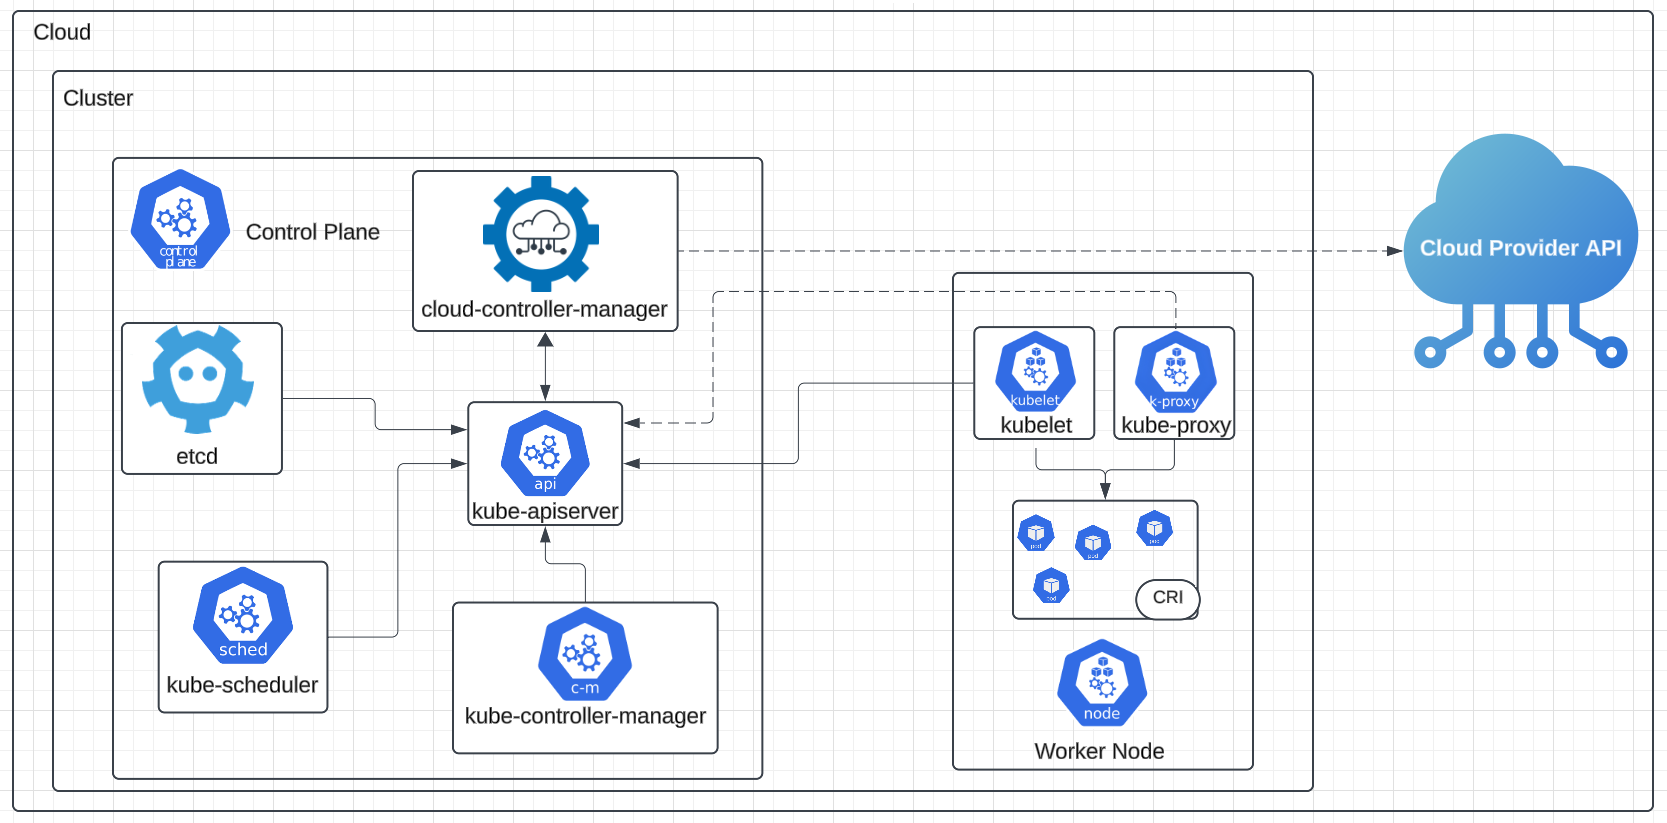
\includegraphics[width=1\columnwidth]{images/kubernetes-cluster-architecture.png}
    \caption{Kubernetes Cluster Architecture \cite{KubernetesArch}\cite{CloudIcon}\cite{K8sIcons}\cite{EtcdIcon}\cite{LucidApp}.}
    \label{fig:k8s_arch}
\end{figure}

In Figure~\ref{fig:k8s_arch} there is graphical representation of Kubernetes cluster. Not all components shown in the figure are mandatory for Kubernetes to work correctly. At the control plane part, \textit{\nameref{sec:cloudControllerManager}} might not be mandatory, in on-premises configurations where interacting with cloud provider is not needed. On the right side of figure in node representation is \textit{\nameref{sec:kubeProxy}} component, which is not mandatory as some networking plugins can provide own implementation of proxy \cite{KubernetesArch}. This is an example of "Designed for extensibility", where Kubernetes can acquire 3rd-party features without changing its source code \cite{KubernetesDocs}.


%---------------------------------------------------------------------------



\subsection{Control plane}
\label{sec:k8s_cplane}

Control plane is like a brain in Kubernetes cluster. Interaction with cluster using kubectl tool to perform requests is handled by \textit{\nameref{sec:kubeApiServer}}. It is responsible for communication with worker nodes running pods, the smallest unit managed by K8s that has containers inside \cite{KubernetesArch}.

%---------------------------------------------------------------------------

\subsubsection{cloud-controller-manager}
\label{sec:cloudControllerManager}

This component allows Kubernetes clusters to interact with cloud provider's API. It is combined with kube-controller-manager as single binary and can be replicated. This is the only component that talks to the cloud provider, separating other components from direct communication with the cloud. When running without cloud environment this component is absent \cite{KubernetesArch}.

%---------------------------------------------------------------------------

\subsubsection{etcd}
\label{sec:etcd}

Etcd is an open-source distributed key-value store service often used in distributed systems. It is responsible for maintaining both the current state and its previous version in its persistent memory \cite{KubernetesArch}\cite{Etcd}.

%---------------------------------------------------------------------------

\subsubsection{kube-apiserver}
\label{sec:kubeApiServer}

Exposes Kubernetes API to interact with a cluster. Takes responsibility for handling all requests from components and users. This is the component which answers cluster administrator requests sent by kubectl \cite{KubernetesArch}.

%---------------------------------------------------------------------------

\subsubsection{kube-controller-manager}
\label{sec:kubeControllerManager}

Component which runs controller processes. Its compiled binary consists of multiple controllers. Example controllers are \cite{KubernetesArch}:

\begin{itemize}
    \item Node controller -- observes worker nodes if are up and running
    \item Job controller -- responsible for batch execution jobs
    \item EndpointSlice controller -- connects services with pods
\end{itemize}

More controller names can be found in \href{https://github.com/kubernetes/kubernetes/blob/master/cmd/kube-controller-manager/names/controller_names.go}{Kubernetes source code}.

%---------------------------------------------------------------------------

\subsubsection{kube-scheduler}
\label{sec:kubeScheduler}

Takes care of pods which are not assigned to a worker node yet. kube-scheduler is looking for node that meets pod's scheduling requirements and fit a pod on that node. Such a node is called feasible node \cite{KubernetesScheduler}.

%---------------------------------------------------------------------------

\subsection{Nodes}
\label{sec:k8sNodes}
All the below-mentioned components run on every node in a cluster.
%---------------------------------------------------------------------------

\subsubsection{Container runtime}
\label{sec:containerRuntime}

Node's key component, has ability to run, execute commands, manage, and delete containers in efficient way \cite{KubernetesArch}. 

%---------------------------------------------------------------------------


\subsubsection{kube-proxy}
\label{sec:kubeProxy}

Create networking rules which allow communicating with pods from outside cluster. If available kube-proxy uses operating system packet filtering to create set of rules. It is also able to forward traffic by itself. This component is optional, can be replaced with a different one if the desired one implements key features. \cite{KubernetesArch}.

%---------------------------------------------------------------------------

\subsubsection{kubelet}
\label{sec:kubelet}

It is responsible for managing containers inside pod on its node. Uses Container Runtime Interface to communicate with containers \cite{KubernetesArch} \cite{KubernetesCRI}.

%---------------------------------------------------------------------------

\subsection{Objects}    
\label{sec:k8s_objects}

\subsubsection{Namespace}
\label{sec:namespace}

The purpose of namespace object is to isolate groups of resources like pods, deployments, services etc. in a cluster. It helps to organize clusters into virtual sub areas of working space. If \textit{\nameref{svc}} is created in some custom namespace <service-name>.<namespace-name>.svc.cluster.local DNS entry within cluster is created \cite{KubernetesNamespaces}.

\subsubsection{Pods}
\label{sec:pods}

Pods are the smallest deployable objects in Kubernetes. They contain one or more containers, which can communicate with each other using localhost interface. Because they share IP addresses, they cannot use the same ports. It is useful when our service consists of two applications coupled together. For example, there is a pod which has two containers, one responsible for compiling code, the second one is creating a cache entry from compiled object and uploading it to some data storage. It is more logical to share data among containers in a pod than on node between pods, as it is easier. Scaling is simpler, as it involves replicating a single pod instead of managing two separate pods. Moreover, communication between applications happens using the localhost interface. In scenario where there are two pods, each with one container, ClusterIP \textit{\nameref{svc}} is needed. However, the most common approach is to run one container per pod, where a pod is just managing wrapper for containerized application. Also, rather than creating pod directly it is more common to use workload resource like \textit{\nameref{deployment}} \cite{KubernetesPods}. 


\subsubsection{ReplicaSet}
\label{replicaset}

Basically \textit{\nameref{replicaset}} consists of pod template and runs desired number of pods \cite{KubernetesReplicaSet}. 


\subsubsection{Deployment}
\label{deployment}

Deployment is a higher-level abstraction over \textit{\nameref{replicaset}}, that manages its lifecycle. It provides more features like rolling back an app, as it keeps history of configurations \cite{KubernetesDeployments}.

\subsubsection{DaemonSet}
\label{daemonset}

Running pods using DaemonSet guarantees that every node will have a copy of the desired pod (if resource requirements are met etc.). It can automatically add or remove pods if the number of nodes changes. The typical usage is creating monitoring pod on every node \cite{KubernetesDaemonSet}. 


\subsubsection{StatefulSet}
\label{statefulset}

StatefulSet, unlike a \textit{\nameref{deployment}}, is stateful. It saves an identity of each pod and if e.g., some persistent storage is assigned to specific e.g., database pod, when it dies, Kubernetes will recreate the pod on the same node as before \cite{KubernetesStatefulSet}.

\subsubsection{Job}
\label{job}

Runs pod that does one task and exists. Kubernetes will retry execution if pod fails specific number of tries set in its configuration \cite{KubernetesJobs}.

\subsubsection{CronJob}
\label{cronjob}
Behaves like \textit{\nameref{job}} but can regularly run at specified intervals for tasks like database backups or log rotation \cite{KubernetesCronJob}. 

\subsubsection{Service}
\label{svc}

Service exposes an application running inside a cluster by using an endpoint. As a pod is ephemeral resource and its address changes sometimes (e.g., when pod is recreated), it is better to create DNS name that resolves IP address. Moreover, the service will not advertise unhealthy pods. Usually, a service exposes one port per service, but for example web app might expose HTTP and HTTPS ports. There are four types of services \cite{KubernetesService}. 


\begin{enumerate}
    \item ClusterIP -- makes one pod available to other inside cluster by exposing application using inter-cluster IP address. Although it is oriented to be accessible within the cluster, objects like \textit{\nameref{ingress}} or \textit{\nameref{gatewayapi}} can expose service to the outside.
    \item NodePort -- by default allocates port (from range 30000-32767) to publish service on every node's IP address. In this scenario every node on the specified port acts like a proxy to the deployed app.
    \item LoadBalancer -- Kubernetes does not provide load balancer by default and when creating such a service it interacts with cloud provider to create external service for traffic balancing. A load balancer can be installed inside cluster.
    \item ExternalName -- allows pods inside Kubernetes to access external service using defined name rather than using IP address 
\end{enumerate}

%---------------------------------------------------------------------------



\subsection{Cluster networking}
\label{sec:k8s_networking}

Networking is the most important thing in Kubernetes, the whole point is to obtain reliable and robust communication among containers, pods, services, nodes, and external systems in a cluster \cite{KubernetesClusterNetworking}. There are four types of network communication: \cite{KubernetesClusterNetworking}:

\begin{enumerate}
    \item container-to-container -- communicates by sharing network resources inside a pod
    \item Pod-to-Pod -- every pod can communicate with any other pod without the need to use NAT as every of them has its own IP address \cite{IBMKubernetesNetworking}.
    \item Pod-to-Service -- covered by service type ClusterIP, which provides inter-cluster IP address
    \item External-to-Service -- held by services type NodePort and Loadbalancer, which expose pod to the outside
\end{enumerate}
Kubernetes allocates IP addresses to nodes, services, and pods \cite{KubernetesClusterNetworking}:
\begin{itemize}
    \item \textit{\nameref{sec:kubelet}} or \textit{\nameref{sec:cloudControllerManager}}, depending on local or cloud infrastructure allocates IP address for nodes
    \item \textit{\nameref{sec:kubeApiServer}} allocates IP address for services
    \item for allocation of IP address to pod is responsible networking plugin which is an implementation of \textit{\nameref{sec:cni}}
\end{itemize}


%---------------------------------------------------------------------------

\section{The concept of traffic engineering in Kubernetes}
\label{sec:trafficConcept}

Traffic Engineering is a key concept in Kubernetes to provide production-ready, reliable, and efficient network. In this section ingress and egress traffic will be explained.

%---------------------------------------------------------------------------

\subsection{Ingress traffic management}
\label{sec:ingressTrafficMngmnt}

\subsubsection{Ingress}
\label{ingress}

Ingress is an object that manages outside cluster access to services inside a cluster. It is a single point of entry to route traffic to specified pod based on configuration. This is only a higher abstract object that specifies routing rules in cluster. Real functionalities are provided by an \textit{\nameref{ingresscontroller}}. Nowadays the development of Ingress is frozen, Kubernetes authors pay attention to its successor a \textit{\nameref{gatewayapi}} \cite{KubernetesIngress}.

\subsubsection{Ingress Controller}
\label{ingresscontroller}

Ingress Controller fulfills an \textit{\nameref{ingress}} and starts serving an application which performs configured rules. Any implementation has its own features, but common functionalities are L4/L7 load balancing, host and path-based routing, SSL termination. This is the real application that runs in a pod. Ingress Controller must be installed manually and is not part of Kubernetes, however the container orchestration tool developers maintain \href{https://github.com/kubernetes-sigs/aws-load-balancer-controller#readme}{AWS}, \href{https://github.com/kubernetes/ingress-gce/blob/master/README.md#readme}{GCE}, and \href{https://github.com/kubernetes/ingress-nginx/blob/main/README.md#readme}{nginx} ingress controllers \cite{KubernetesIngress}\cite{KubernetesIngressControllers}. 


\subsubsection{Gateway API}
\label{gatewayapi}

The functionalities of Gateway API are so wide, that the Kubernetes authors use term "project". The project focuses on L4 and L7 routing in a cluster. It succeeds \textit{\nameref{ingress}}, Load Balancing and service mesh APIs. The Gateway API resource model is role-oriented \cite{KubernetesGatewayAPI}.

\begin{figure}[tbh]
    \centering
    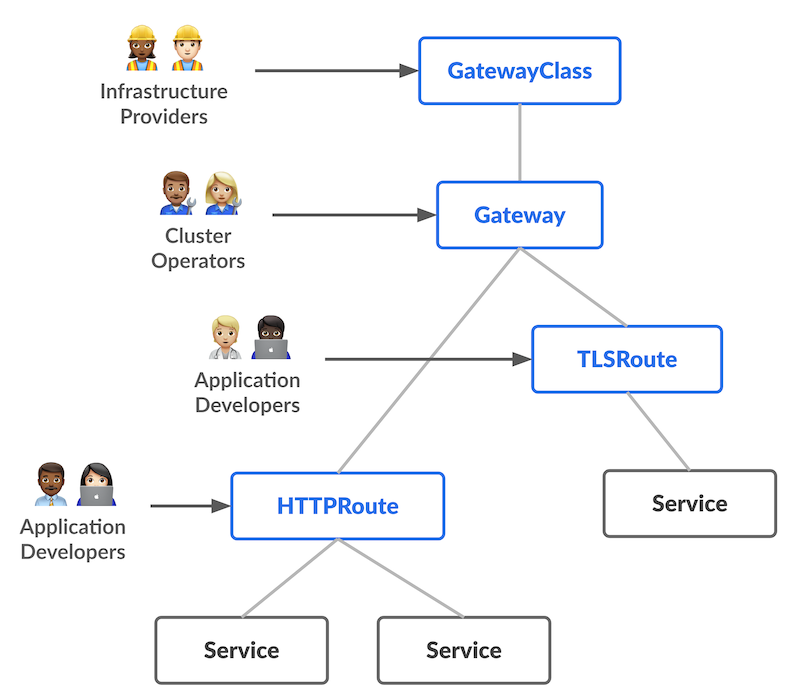
\includegraphics[width=0.7\columnwidth]{images/gateway-api-resource-model.png}
    \caption{Gateway API roles-oriented resource model \cite{LucidApp}\cite{KubernetesGatewayAPI}\cite{PersonIcon}.}
    \label{fig:gatewayApiResourceModel}
\end{figure}

The model focuses on 3 separate groups of people who interact with a cluster on various levels. 

On a top of Figure~\ref{fig:gatewayApiResourceModel} there are infrastructure providers, who provide GatewayClass resource. They are responsible for the overall multiple clusters, rather than ensuring developers can access pods correctly \cite{KubernetesGatewayAPI}. The GatewayClass resource is a class of Gateway which can be created. It defines specific types of load balancing implementations and provides clear explanation of capabilities available in Kubernetes resource model. The functionality is like \textit{\nameref{ingress}} \cite{KubernetesGatewayAPI} \cite{KubernetesGatewayClass}. There can be more than one GatewayClasss created. \cite{KubernetesGatewayAPI}. 


Cluster operators are in the middle of Figure~\ref{fig:gatewayApiResourceModel}, they make sure that cluster meets requirements for several users. As maintainers define Gateway resource, some load balancing system is provisioned by GatewayClasss. Gateway resource defines specific instance which will handle incoming traffic. Allows defining specific protocol, port or allowed resources to route inbound traffic \cite{KubernetesGatewayAPI} \cite{KubernetesGateway}.

End users specified on Gateway API resource model in Figure~\ref{fig:gatewayApiResourceModel} are application developers. They focus on serving applications to the clients by creating a resource named HTTPRoute. The resource defines HTTP routing from defined gateway to end API objects like service. It can to split traffic using "weight" as a key, which represents the percentage of the total traffic to be routed. GRPCRoute is similar, but operates on different protocols. \cite{KubernetesGatewayAPI} \cite{KubernetesHTTPRoute}. 



Gateway API is not an API Gateway. An API Gateway in general is responsible for routing, load balancing, information exchange manipulation and much more depending on specific implementation. Gateway API is set of three resources mentioned earlier, which creates a role-oriented Kubernetes service networking model. Creators of Gateway API provide a clear explanation: "Most Gateway API implementations are API Gateways to some extent, but not all API Gateways are Gateway API implementations" \cite{KubernetesGatewayAPI}. 

%---------------------------------------------------------------------------

\subsection{Egress traffic management}
\label{sec:egressTrafficMngmnt}

Egress traffic refers to connections which leave cluster and are initiated inside by pods. In contrast to the Ingres object, in Kubernetes there is no Egress resource, outgoing traffic route logic is implemented by Container Network Interface plugin. The most common approach in managing egress traffic is to use Kubernetes Network Policies to deny all outgoing traffic and then allow only key connections. The limitation is that all external services need to be specified with IP address in policies. Any change in external resource's IP requires a change in policy configuration. If any pod is trying to access external service, source network access translation (SNAT) needs to be performed to map inter-cluster pod IP to externally routed nodes IP. When the response is accessing cluster, SNAT is performing translation in opposite way. Another key egress concept in Kubernetes is an egress gateway. This is a node which proxies outgoing traffic from a cluster, specified by provided configuration (e.g., by labeling pods, depends on CNI implementation). The important thing is that the internal pod's IP address is masqueraded into IP address of an egress gateway, outside peer does not see ephemeral IP of a pod. Egress gateway is also a CNI specific implemented resource. \cite{CalicoEgress} \cite{CiliumEgressGateway}. 


%---------------------------------------------------------------------------

\section{Container network interface (CNI)}
\label{sec:cni}
CNI is standardized by Cloud Native Computing Foundation set of API rules which defines container networking. CNI is responsible for pod-to-pod communication, which includes assigning IP addresses, configuring network interface inside container and routing \cite{IBMKubernetesNetworking}. 



%---------------------------------------------------------------------------

\subsection{Overview of selected CNI plugins}
\label{sec:cni_overview}


\begin{table}[h!]
    \centering
    \caption{Comparison of Antrea and Cilium \cite{Antrea}\cite{CiliumBGP}\cite{CiliumEgressGateway}\cite{CiliumGatewayAPI}\cite{CiliumEncryption}.}
    \resizebox{\textwidth}{!}{%
    \begin{tabular}{|l|l|l|}
    \hline
    \textbf{Feature/Plugin}              & \textbf{Antrea}                                         & \textbf{Cilium}                                \\ \hline
    \textbf{Dataplane}            & Open vSwitch                                            & eBPF                                           \\ \hline
    \textbf{Encapsulation}        & VXLAN or Geneve                                         & VXLAN or Geneve                                \\ \hline
    \textbf{Encryption}           & IPsec or WireGuard tunnels                              & IPsec or WireGuard tunnels                     \\ \hline
    \textbf{Security}             & Extends Kubernetes Network Policies                     & Advanced security policies                     \\ \hline
    \textbf{Observability}        & Theia and Grafana for visualization                     & Hubble                                         \\ \hline
    \textbf{Purpose}              & Simplified Kubernetes networking management             & For large-scale cluters                        \\ \hline
    \textbf{Additional features}  & Network policies for non-Kubernetes nodes               & BGP to advertise network outside cluster       \\ \hline
    \textbf{Gateway API}          & No support                                              & Fully supports Gateway API                     \\ \hline
    \textbf{Egress Gateway}       & Basic egress gateway capabilities                       & Advanced egress gateway support                \\ \hline
    \end{tabular}}
    \label{tab:antrea_cilium}
\end{table}


Antrea is an open-source CNI plugin which is built on Open vSwitch which requires kernel version greater than 4.6 \cite{Antrea} \cite{AntreaStart}. OvS is a virtual switch with capability of handling traffic flow between virtual machines and containers \cite{OvS}. Antrea's focus is L3/L4 networking and security services, such as network policies. The resource is responsible for managing traffic flow between pods. By default, every pod can communicate with any other pod, but network policies can specify if pod A is able to talk to pod B \cite{KubernetesNetworkPolicies}. Consider scenario with three pods, client, frontend, and backend. There is no need to allow client communication directly with backend, so network policies allow traffic flow from client to frontend and direct communication with backend is not allowed \cite{CalicoNetworkPolicies}. 


Cilium, open-source CNI which uses eBPF (extended Barkeley Packer Filter) for packet processing, security and deep observability using Hubble \cite{CiliumOverview}. Some environments may not be suitable because Cilium requires a kernel version of 5.4 or higher \cite{CiliumInstall}. eBPF is a technology that allows running defined programs, with custom logic inside operating system kernel in privileged context without need of any kernel source code changes or loading modules. Lack of switching between kernel and user space, which reduces latency \cite{eBPF}. 

Figure~\ref{fig:ebpf_routing}, shows standard container networking on the left side and Cilium eBPF container networking on the right. The whole point of eBPF networking is skipping overhead that comes from iptables. Moreover, eBPF implements hash tables for storing routing policies, which time complexity is O(log n), compared to iptables array O(n). It makes clear that large-scale clusters will benefit from using eBPF \cite{IsovalentHash}. 

\begin{figure}[H]
    \centering
    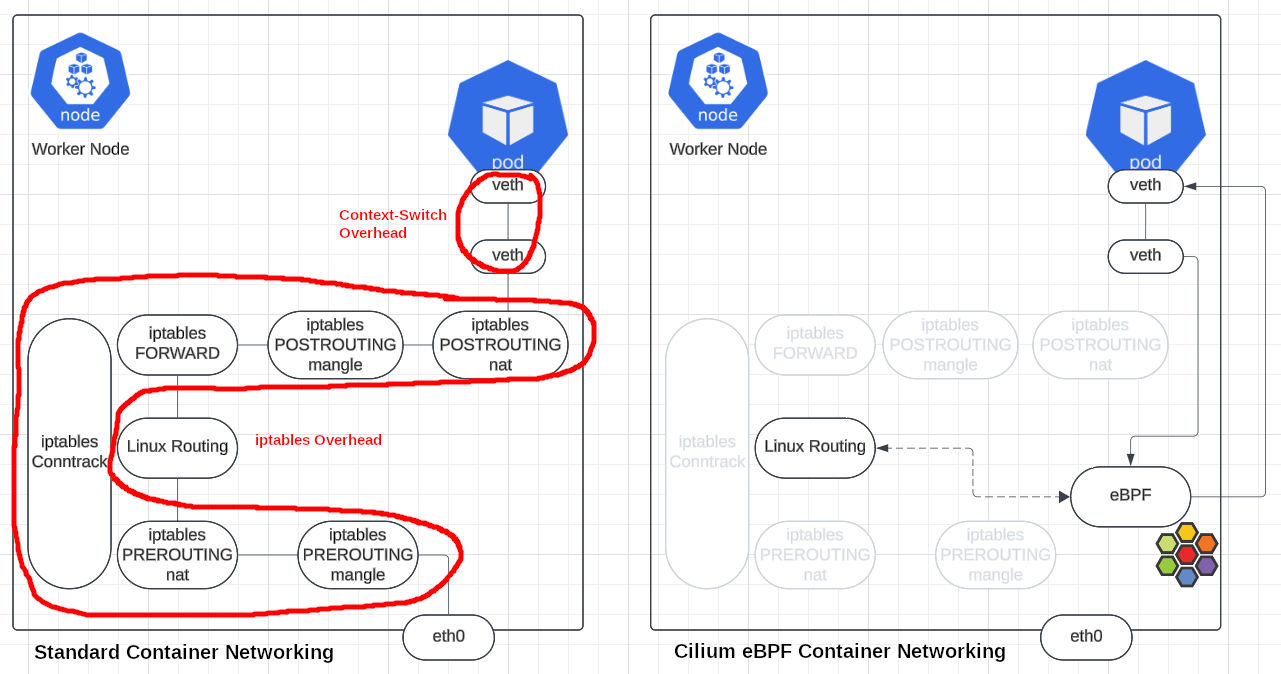
\includegraphics[width=0.9\columnwidth]{images/ebpf_hostrouting.png}
    \caption{Cilium eBPF host-routing \cite{K8sIcons}\cite{LucidApp}\cite{CiliumCNIBenchmark}.}
    \label{fig:ebpf_routing}
\end{figure}



%---------------------------------------------------------------------------

\section{Related work}
\label{sec:realted_work}

As discussed in \cite{dakic2024performance} the performance of different CNIs can vary widely, some CNIs performing two to three times better than others, making it essential to choose the right plugin for a particular workload. Authors say that developing automated methodology of CNI plugin evaluation is a key aspect, specifically in large High-Performance Computing (HPC) environments. This allows for reproducible and consistent tests across different configurations, reducing the overhead of manual testing. To achieve that, tools like Ansible can be helpful. They state that Linux Kernel or NIC can be a bottleneck in networking performance, so they extend maximum buffer size, scale TCP window, disable TCP Selective Acknowledgement, increase SYN Queue Size, or enable Generic Receive offload. The paper shows results of comparison four CNI plugins, such as Antrea, Cilium, Calico, Flannel using TCP/UDP in base and with optimized system settings \cite{dakic2024performance}. 

In \cite{9153266} the authors measure CNI plugins for inter-host and intra-host communication using UDP and TCP protocols. They introduce the concept of CPU cycles per packet (CPP) to evaluate CNI efficiency. They measure CPP spent in each network component using the Linux perf tool. By measuring throughput, RTT, and latency, they compare how different CNI plugins (Flannel, Weave, Cilium, kube-router, Calico) compared to its network models \cite{9153266}. 

Another paper \cite{9309003} of \cite{9153266} authors. Functionality, performance, and scalability are in focus, the scale testbed up to 99 Iperf client and 99 Iperf server pod, mentioning that 100 pods are Kubernetes one node limit \cite{9309003}. 

The authors of \cite{10138542} state that in the coming years, fifth generation mobile networks (5G) will deploy a significant part of their infrastructure in the cloud-native platforms, resulting in the creation of large-scale clusters. Such production environments containing thousands of pods require creating stable, reliable, and efficient networks. They do not focus their attention on which CNI uses in this scenario, rather highlight such concepts as highly performant networking, security, and observability. Authors state that the key to meet this expectation is eBPF (extended Barkeley Packet Filter) \cite{10138542}. 

\chapter{Introduction to Egress and Ingress Scenarios in Selected CNI Plugins}
\label{cha:introScenarios}
In modern Kubernetes networking, managing traffic flow into and out of a cluster is crucial for performance and security. Different CNI plugins provide distinct mechanisms for controlling network traffic, each offering a unique approach to networking implementation. Understanding how traffic is managed in both ingress and egress scenarios is essential for improving security, optimizing performance, and enhancing overall network efficiency.

\section{Egress scenario: routing outgoing traffic via Egress Gateway}
\label{sec:egress}

The egress gateway can play a key role in a cluster's security. It can enforce routing all outgoing connections initiated within labeled pods through the gateway node. The node can route all outgoing traffic through a security system to scan each packet for potential threats, ensuring that outgoing traffic only accesses secure services outside the cluster.

The IT department of a financial company manages Kubernetes clusters in their local laboratory. The infrastructure is used to create a production-ready, efficient, and secure environment for financial services, where handling sensitive data and adhering to strict regulatory standards is critical. Leaving unmonitored critical traffic leaving the cluster can create vulnerabilities, potentially exposing the system to data exfiltration from financial applications. They decided to analyze all outgoing traffic from financial services pods using intrusion detection system (IDS) software. However, they also provide services that do not require such robust security. Redirecting every request to the traffic analyzer would add unnecessary overhead to exposed applications and cause higher latency. Cluster operators decided to leverage an egress gateway to route all outgoing traffic from financial services into a security tool to monitor and analyze packets. However, end users started complaining that their applications were showing errors like "503 Service Unavailable." The IT administrators began troubleshooting and concluded that the egress gateway was acting as a bottleneck in the cluster. They started searching online for solutions and decided to create separate gateways for each deployment of their services \cite{CalicoEgressDeploy}. End users stopped complaining about poor service availability.

\subsection{Egress gateway in selected CNI plugins}
\label{subsection:egressGateway}

Container Network Interface (CNI) plugins implement their own egress gateways, offering unique features. This section explores the capabilities of the Antrea and Cilium CNI plugins, focusing on how they handle outbound traffic and integrate with other networking components. Understanding these implementations is essential for Kubernetes operators to select the right CNI plugin for their specific requirements.


\subsubsection{Antrea}
\label{subsection:antreaEgress}

The Antrea Egress CRD (Custom Resource Definition) API is a resource that controls how pods in a cluster access external services. This resource specifies which egress IP should be used by selected pods. When a pod communicates with an external network, the traffic is routed through the node that has the specified egress IP (egress gateway). The source IP address of the traffic is then translated to the configured IP address \cite{AntreaEgressArch}.

\begin{figure}[tbh]
    \centering
    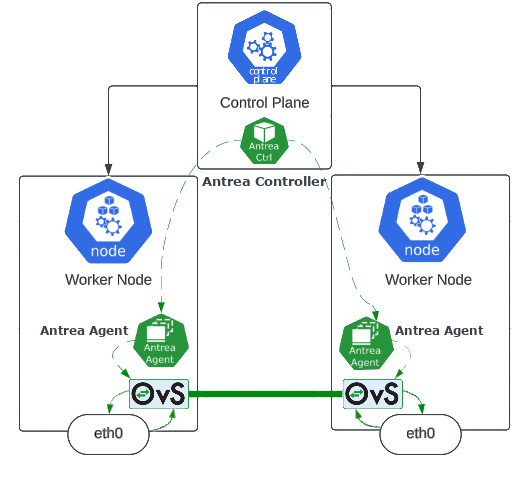
\includegraphics[width=0.6\columnwidth]{images/antrea_overview.png}
    \caption{Antrea Egress Architecture \cite{LucidApp}\cite{AntreaEgressArch}.}
    \label{fig:antreaEgressArch}
\end{figure}


Figure~\ref{fig:antreaEgressArch} shows the architecture of the communication flow when an egress gateway is configured in the Antrea CNI. When a pod running on a Kubernetes node tries to access an external service (assuming it is labeled to route its outbound traffic through the egress node), the traffic is tunneled (through OvS) to the gateway node, and the Antrea Agent performs SNAT. After translation, the next network peer that communicates with the egress gateway will see its IP as the source IP, instead of the IP address of the pod \cite{AntreaEgressArch} \cite{AntreaSNAT} \cite{AntreaArch}.

Let's explain the egress configuration YAML from Listing~\ref{lst:yamlAntreaEgress} \cite{AntreaEgressArch}:
\begin{itemize}
    \item Antrea allows matching the pods that route through the egress gateway based on two criteria:

    \begin{enumerate}
        \item namespaceSelector -- specifies which pods within the specified namespace should redirect outbound traffic.
        \item podSelector -- selects pods with the specified labels. For example, it can match pods labeled with role=web to redirect traffic.
    \end{enumerate}

    \item egressIP -- specifies SNAT IP address of an egress gateway, to which traffic is tunneled
    \item externalIPPool -- name of externalIPPool resource which contains pool of IP addresses to allocate if egressIP is not set
\end{itemize}

It is possible to configure a failover egress gateway node using Antrea. To do this, egressIP and externalIPPool must be set (with egressIP being part of externalIPPool). When the current egress gateway stops working, another node within the externalIPPool will be selected. This infrastructure, with a failover service, is part of a high-availability setup for production environments (useful for the previously mentioned IT department) \cite{AntreaEgressArch}.


\begin{listing}[htb]
    \centering
    \caption{Egress resource example \cite{AntreaEgressArch}.}
    \begin{minted}[gobble=4, frame=single, linenos, fontsize=\scriptsize]{yaml}
    apiVersion: crd.antrea.io/v1alpha2
    kind: Egress
    metadata:
        name: egress-prod-web
    spec:
        appliedTo:
        namespaceSelector:
            matchLabels:
            env: prod
        podSelector:
            matchLabels:
            role: web
        egressIP: 10.10.0.8
        externalIPPool: prod-external-ip-pool
    status:
        egressNode: node01
    \end{minted}
    \label{lst:yamlAntreaEgress}
\end{listing}

The ExternalIPPool resource from Listing~\ref{lst:yamlAntreaExternalIPPool} can be configured with the following fields \cite{AntreaEgressArch}:

\begin{itemize}
    \item ipRanges -- IP pools range can be configured using a pair of IP (start and end), or by setting CIDR (Classless Inter-Domain Routing) range
    \item nodeSelector -- will apply only on nodes specified by this field, e.g., nodes labeled with network-role: egress-gateway
\end{itemize}

\begin{listing}[htb]
    \centering
    \caption{ExternalIPPool resource example \cite{AntreaEgressArch}.}
    \begin{minted}[gobble=4, frame=single, linenos, fontsize=\scriptsize]{yaml}
    apiVersion: crd.antrea.io/v1alpha2
    kind: ExternalIPPool
    metadata:
        name: prod-external-ip-pool
    spec:
        ipRanges:
            - start: 10.10.0.2
              end: 10.10.0.10
            - cidr: 10.10.1.0/28
        nodeSelector:
        matchLabels:
            network-role: egress-gateway
    \end{minted}
    \label{lst:yamlAntreaExternalIPPool}
\end{listing}
  


\subsubsection{Cilium}
\label{subsection:ciliumEgress}

To take advantage of Cilium's egress gateway features, eBPF masquerading must be enabled, and the node's kube-proxy component must be replaced with Cilium's implementation \cite{CiliumEgressGateway}. As shown in Figure~\ref{fig:ciliumEgressArch}, the Cilium agent injects routing information into eBPF maps within the kernel (relying on kernel support for eBPF features). Traffic from worker nodes is redirected to the egress gateway node, where it is SNATed and leaves the cluster. These routes, defined by Cilium policies configured in the control plane, ensure that every node is aware of which pods should redirect traffic to the designated egress node \cite{CiliumEgressGateway}. For node-to-node communication, Cilium encapsulates all traffic using UDP-based VXLAN or Geneve protocols \cite{CiliumRouting}.

\begin{figure}[tbh]
    \centering
    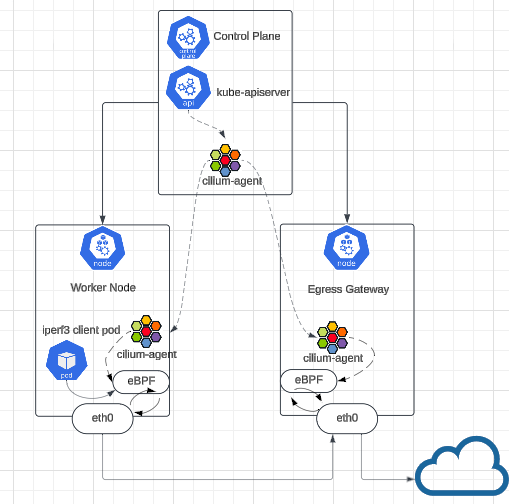
\includegraphics[width=0.9\columnwidth]{images/cilium_egress.png}
    \caption{Cilium Egress Architecture \cite{K8sIcons}\cite{LucidApp}\cite{CloudIcon2}\cite{CiliumEgressGatewayBlog}.}
    \label{fig:ciliumEgressArch}
\end{figure}

Similar to Antrea egress resources, Cilium has its own CiliumEgressGatewayPolicy present on Listing~\ref{lst:yamlCiliumEgressGatewayPolicy} \cite{CiliumEgressGateway}:

Cilium allows matching the traffic that route through the egress gateway by \cite{CiliumEgressGateway}:
\begin{itemize}
    \item podSelector -- matching pods based of used selector, like previous matching labels in Antrea, or by matching expressions (key operator, values). More than one podSelector can be used
    \item destinationCIDRs -- an app in pod is requesting some external service, if this resource is match by defined CIDR, the request is routed to egress gateway. For 0.0.0.0/0 all traffic is outgoing by egress gateway. Setting excludedCIDRs is possible to exclude some IPs.
\end{itemize}

Selecting an egress gateway can be done in three ways: by matching node labels, using IP address in egressIP field (as in Antrea) or by interface name \cite{CiliumEgressGateway}. 

\begin{listing}[htb]
    \centering
    \caption{Egress resource example \cite{AntreaEgressArch}.}
    \begin{minted}[gobble=4, frame=single, linenos, fontsize=\scriptsize]{yaml}
    apiVersion: cilium.io/v2
    kind: CiliumEgressGatewayPolicy
    metadata:
    name: egress-sample
    spec:
    selectors:
    - podSelector:
        matchLabels:
            org: empire
            class: mediabot
            io.kubernetes.pod.namespace: default
        matchExpressions:
            - {key: testKey, operator: In, values: [testVal]}
            - {key: testKey2, operator: NotIn, values: [testVal2]}
    destinationCIDRs:
    - "0.0.0.0/0"
    excludedCIDRs:
    - "192.168.1.0/24"
    egressGateway:
        nodeSelector:
        matchLabels:
            node.kubernetes.io/name: a-specific-node
        egressIP: 10.168.60.100
    \end{minted}
    \label{lst:yamlCiliumEgressGatewayPolicy}
\end{listing}


Both Antrea and Cilium allow us to configure an egress gateway in multiple ways. Cilium offers more flexibility in defining which traffic should be routed through the egress gateway. Unlike Antrea, Cilium can specify traffic by destination CIDR. While Cilium provides more capabilities for matching egress traffic, Antrea's implementation allows for the creation of a failover node, which will route traffic if the primary one fails. Creating a high-availability egress gateway in Cilium is possible only with the enterprise, paid version of the plugin. Additionally, Cilium leverages eBPF, which is designed for large-scale clusters \cite{CiliumOverview}. It is not clear which egress gateway CNI implementation is the best to use, as each has its advantages and drawbacks. In the next section, both gateways will be evaluated using networking tools in a local environment.




\section{Ingress scenario: splitting incoming traffic via Gateway API}
\label{sec:ingress}

The Gateway API, as a successor to the Ingress object, provides enhanced features for traffic management and introduces a role-oriented approach to separate Kubernetes user and operator concerns. It supports traffic splitting, header modification, and URL rewriting. Additionally, the Gateway API supports key protocols such as HTTP, HTTPS, TCP, UDP, and gRPC. With its wide range of features, it can be used in various ways \cite{CiliumGatewayAPIBlog}.

%---------------------------------------------------------------------------
\subsubsection{Canary Deployment}
\label{subsubsection:canary}

Canary Deployment is one of the most common methods used to roll out a new application version to end users, ensuring that everything is working as expected before the full release. The core idea is to release new versions of software only to a small group of users, leaving most users unaware of the new release \cite{Canary}.

This is where the traffic splitting feature of the Gateway API can be used \cite{CiliumTrafficSplitting}. There are typically five stages in the deployment process \cite{Canary}:

\begin{itemize}
    \item Initial state -- The stable version of the application is served.
    \item Canary stage -- The updated version of the application is visible only to 5\% of users. As some users interact with the newly provisioned software, the most common errors should be visible (if any).
    \item Early stage -- The second stage of canary deployment, where the new app is available to 25\% of total connections. At this point, less frequent bugs may be observed.
    \item Mid stage -- The app is available to 50\% of end users. Half of the traffic is routed to the latest version of the app. At this point, the performance of the rolled-out software is monitored.
    \item Late stage -- Most of the traffic (75\%) is handled by the recent version of the application. This stage precedes the full release of the new software.
    \item Full stage -- 100\% of users are served the new application version.
\end{itemize}

If any anomalies are detected during any stage of the canary deployment, the new application version should be immediately rolled back.

The Gateway API is not designed for software deployment and does not have capabilities for rolling back applications automatically. In this usage, the gateway is used only for weighted traffic splitting.

%---------------------------------------------------------------------------

\subsubsection{Traffic Mirroring with Gateway API}
\label{subsubsection:mirroring}

A company is offering a weather API, but not all endpoints are publicly available. Some features are secured and paid. Securing these paid interfaces is not as critical as securing more sensitive and confidential data. Recently, the company decided to start analyzing incoming traffic on these secured endpoints to ensure that only authorized requests are being handled. However, the company does not have the infrastructure capabilities to analyze all incoming traffic for these endpoints. As their services are HTTP-based inside a Kubernetes cluster, they can take advantage of the Gateway API’s traffic splitting feature. The security team decided to route 40\% of the incoming traffic to a traffic analyzer to evaluate whether and how requests might bypass the paywall. The cluster management team (acting as both infrastructure providers and cluster operators, according to the roles in the Gateway API model) decided to split the traffic using the Gateway API, as they need general usage of the API Gateway (since the company offers RESTful APIs). Pure traffic splitting is not sufficient in this case because all incoming traffic must be handled in response. The solution is to split 40\% of the traffic to a different Kubernetes service, mirror the traffic to the analyzer, and then route it back to the pod containing the application. While the cluster managers implement the second deployment to mirror requests to the traffic analyzer, the app developers created an HTTPRoute object with appropriate weights for each of the services. Figure~\ref{fig:mirroringImg} shows how the cluster infrastructure might look in this case.


\begin{figure}[H]
    \centering
    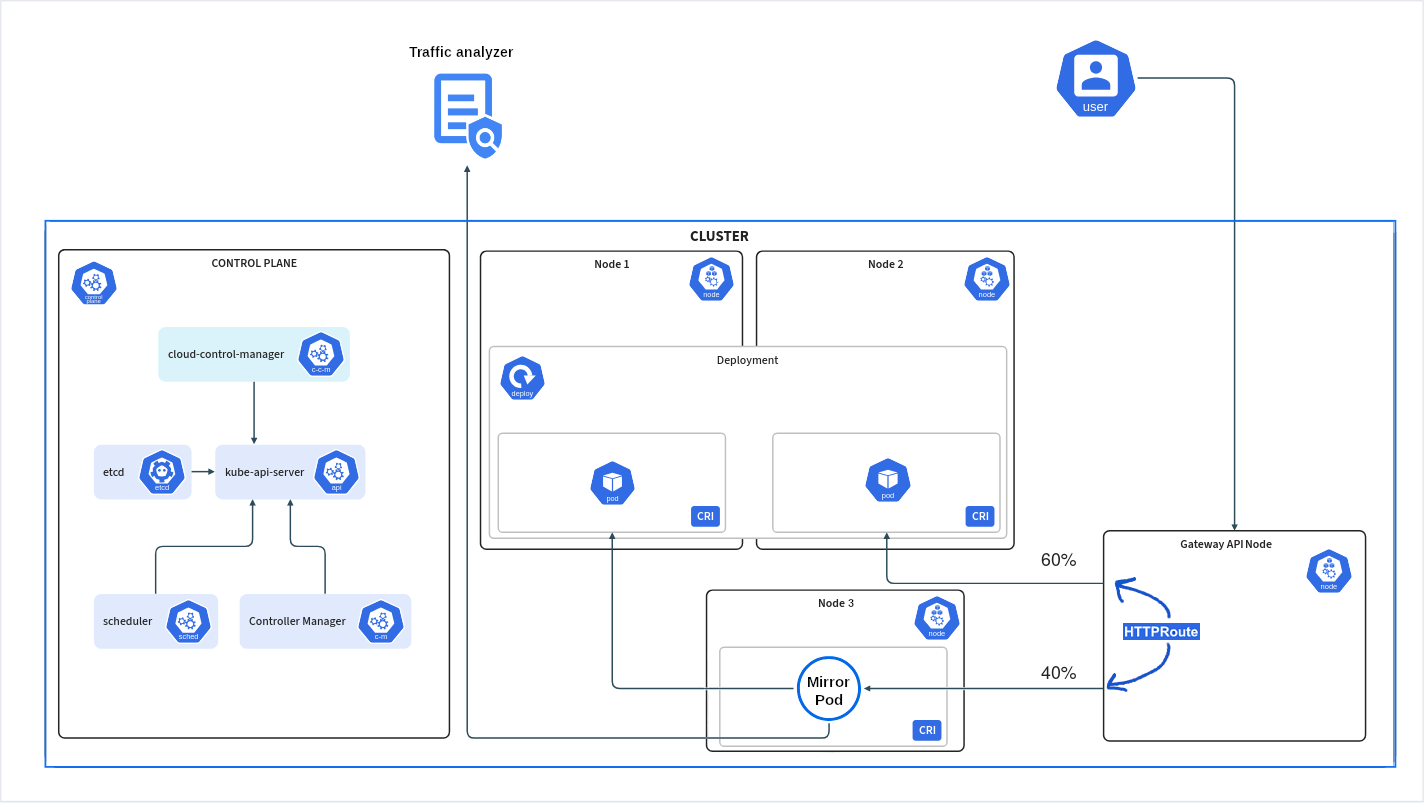
\includegraphics[width=1\columnwidth]{images/ingress.png}
    \caption{Example Kubernetes cluster with traffic mirroring \cite{KubernetesArch}\cite{K8sIcons}\cite{LucidApp}.}
    \label{fig:mirroringImg}
\end{figure}

%---------------------------------------------------------------------------

\subsection{Traffic splitting in selected CNI plugins}
\label{subsection:trafficSplitting}

Unfortunately, the Antrea plugin does not provide an implementation of the Gateway API. In fact, Cilium is the only CNI plugin that offers this functionality. To evaluate the cluster networking implementation with Antrea CNI, the NGINX Gateway Fabric can be used instead.



%---------------------------------------------------------------------------
\subsubsection{Antrea + NGINX}
\label{subsection:antreaIngress}

Figure~\ref{fig:canaryAntreaImg} shows an example cluster where the Gateway API is configured to work in the canary stage. Antrea CNI is installed, and the antrea-ctrl and antrea-agent pods are deployed on the nodes. OvS tunneling among nodes is set up \cite{Antrea}. On the control plane node, the NGINX Gateway API is deployed as a pod \cite{NGINX}. This differs from Cilium, where the Gateway API is not run as a single pod \cite{CiliumGatewayAPI}. In this setup, traffic is processed by the NGINX Gateway API pod, while Antrea handles the networking stack, integrating with NGINX to manage traffic routing.

\begin{figure}[H]
    \centering
    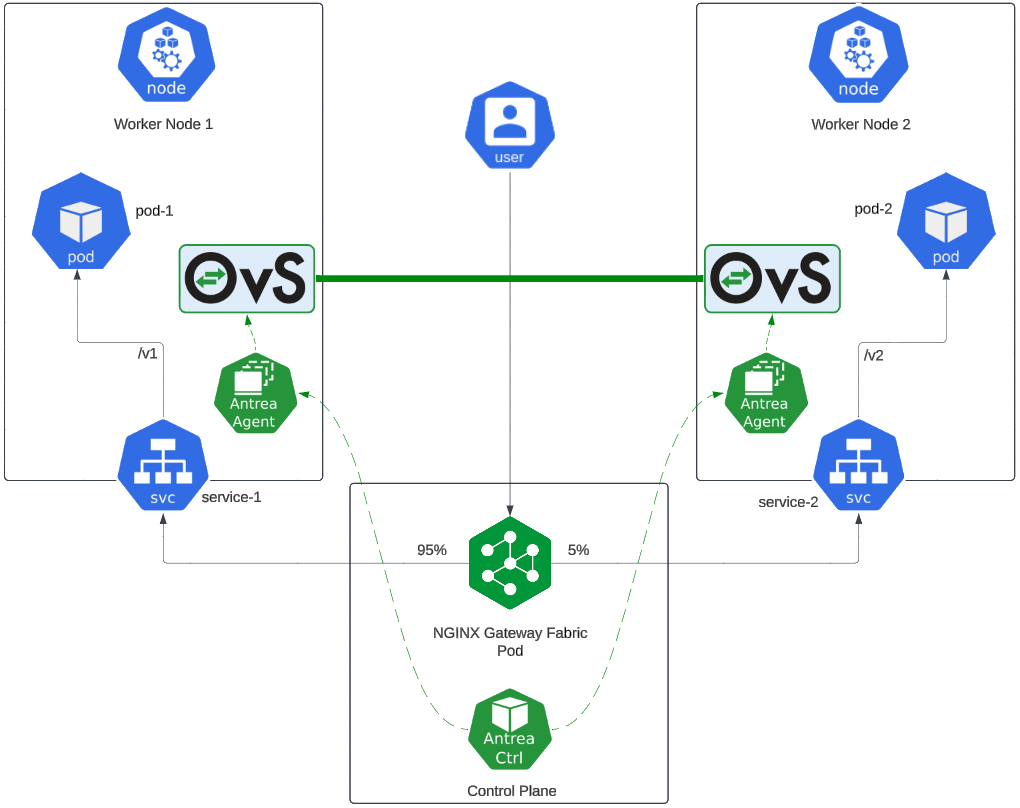
\includegraphics[width=1\columnwidth]{images/antrea-nginx.png}
    \caption{Example Kubernetes cluster with Antrea CNI and NGINX Gateway Fabric in canary stage of canary deployment \cite{KubernetesArch}\cite{K8sIcons}\cite{LucidApp}\cite{AntreaEgressArch}.}
    \label{fig:canaryAntreaImg}
\end{figure}

\begin{listing}[htb]
    \centering
    \caption{Egress resource example \cite{AntreaEgressArch}.}
    \begin{minted}[gobble=4, frame=single, linenos, fontsize=\scriptsize]{yaml}
    apiVersion: gateway.networking.k8s.io/v1
    kind: HTTPRoute
    metadata:
        name: current-weather-route
    spec:
        parentRefs:
        - name: nginx-gw
        rules:
        - matches:
            - path:
                type: PathPrefix
                value: /getCurrentWeather
            backendRefs:
            - kind: Service
                name: current-weather-pod-1
                port: 8080
                weight: 95
            - kind: Service
                name: current-weather-pod-2
                port: 8090
                weight: 5
    \end{minted}
    \label{lst:yamlAntreaIngressCanaryHTTPRoute}
\end{listing}
%---------------------------------------------------------------------------

\subsubsection{Cilium}
\label{subsection:ciliumIngress}

In Figure~\ref{fig:ciliumDataflow}, an example canary cluster stack using the Cilium plugin is presented. The arrows represent the real data traffic flow, while the dashed arrows indicate the configuration flow. The HTTPRoute resources are pulled by the cilium-agent, which prepares the configuration and injects it into the Envoy proxy and eBPF. When Envoy receives an incoming request, it understands the traffic-splitting ratio and decides whether to route the traffic to a local pod or to a different pod, as specified in the HTTPRoute configuration \cite{CiliumComponents}. The HTTPRoute resource for the Cilium Gateway API will look almost exactly the same as in Listing~\ref{lst:yamlAntreaIngressCanaryHTTPRoute}, with the only difference being the parentRefs name, which defines which Gateway is being used.

\begin{figure}[H]
    \centering
    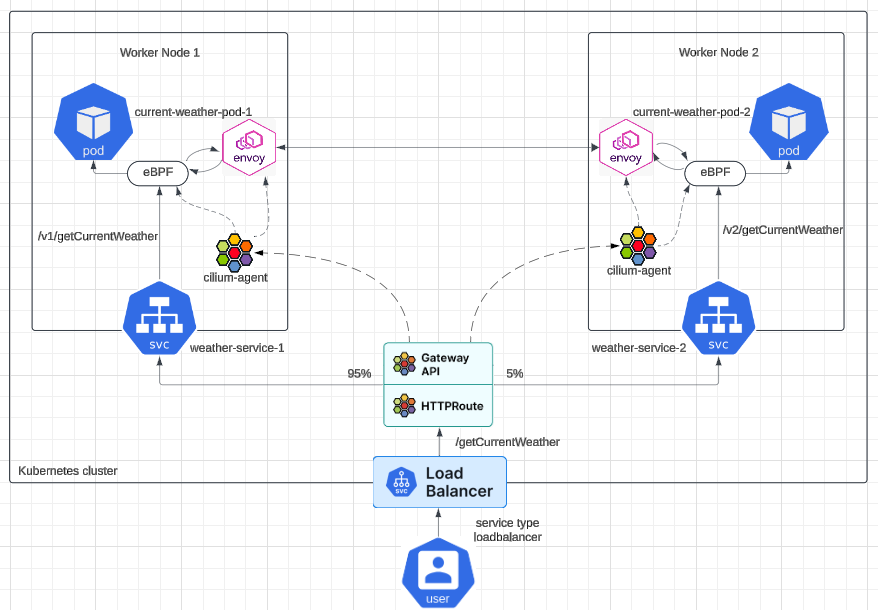
\includegraphics[width=1\columnwidth]{images/cilium_dataflow.png}
    \caption{Example Kubernetes cluster with Cilium CNI in canary stage of canary deployment \cite{K8sIcons}\cite{LucidApp}\cite{CiliumEgressGatewayBlog}.}
    \label{fig:ciliumDataflow}
\end{figure}

%---------------------------------------------------------------------------
\chapter{Implementing Egress and Ingress Scenarios Using Selected CNI Plugins}
\label{cha:practical_impl}

This chapter presents the implementation of both egress and ingress scenarios. The egress scenario will be executed locally, while the ingress scenario will be deployed both on local infrastructure (personal laptop) and in the public cloud (Azure). The tools used in these implementations, along with example configurations, will be described.

The Kubernetes cluster will run on a local laptop with the following specifications:
\begin{itemize}
  \item CPU: AMD Ryzen 5 3500U 8 CPUs
  \item RAM: 20 GB
  \item Storage: 256 GB SSD
  \item Operating System: Fedora 40 with kernel 6.10.11
\end{itemize}

The cloud infrastructure consists of two AKS nodes (virtual machines) of type Azure Standard\_A2\_v2. Each VM has the following specifications:
\begin{itemize}
  \item CPU: 2 vCPUs
  \item RAM: 4 GB
  \item Storage: Standard SSD
  \item Operating System: Ubuntu 22.04
\end{itemize}




%---------------------------------------------------------------------------


\section{Tools and automation}
\label{sec:tools}

In this section, the tools used to provision the egress and ingress implementations will be described. A Kubernetes cluster will be created to simulate the scenarios, with Terraform, an Infrastructure as Code (IaC) tool, used to provision and interact with the cluster. Additionally, Ansible will be used to create and configure the cluster setup, as well as to run Terraform and performance tools.


%---------------------------------------------------------------------------

\subsubsection{Ansible}
\label{sec:ansible}

Ansible is an open-source tool that automates the provisioning and configuration of infrastructure. Configuration in Ansible is written in playbooks, which are YAML files that serve as blueprints containing a set of instructions to be executed. Each playbook consists of one or more plays, and each play describes a set of tasks to be performed on a group of targeted hosts \cite{AnsibleDocs}.

\begin{listing}[htb]
    \centering
    \caption{Example Ansible playbook \cite{AnsibleDocs}.}
    \begin{minted}[gobble=4, frame=single, linenos, fontsize=\scriptsize]{yaml}
    - name: Create openstack instance and assign floating ip
      hosts: "{{ openstack_pool | default('localhost') }}"
      var_files:
        - ./vars/auth.yml
      become: yes
  
      tasks:
        - name: Create the OpenStack instance
          openstack.cloud.server:
            state: present
            name: " {{ inventory_hostname }}"
            key_name: "{{ key_name }}"
            network: "{{ network_name }}"
            auth:
              auth_url: "{{ auth_url }}"
              username: "{{ username }}"
              password: "{{ password }}"
              project_name: "{{ project_name }}"
  
      roles:
        - assign_floating_ip

    \end{minted}
    \label{lst:exampleAnsiblePlaybook}
\end{listing}

\begin{listing}[htb]
    \centering
    \caption{Example Ansible inventory \cite{AnsibleDocs}.}
    \begin{minted}[gobble=4, frame=single, linenos, fontsize=\scriptsize]{yaml}
    [openstack_pool]
    instance-1.example.com key_name=ansible_key network_name=my-network ansible_host=10.10.10.10
    instance-2.example.com key_name=ansible_key network_name=my-network ansible_host=10.10.10.20
    \end{minted}
    \label{lst:exampleAnsibleInventory}
\end{listing}


Listing~\ref{lst:exampleAnsiblePlaybook} shows an example Ansible playbook configuration. The hosts field defines the group of objects on which the configuration script will be executed. In this case, instances specified in the openstack\_pool group in the Ansible inventory, shown in Listing~\ref{lst:exampleAnsibleInventory}, will be created when the playbook is run. The vars\_files option allows for attaching files that contain variables, such as authentication credentials required to access the OpenStack cloud. The become directive is used to execute the script as the root user. The tasks and roles sections define the actual tasks. These can be specified directly in the tasks section or through roles. In this example, the script is referenced from ./roles/assign\_floating\_ip/tasks/main.yaml \cite{AnsibleDocs}.


\subsubsection{Iperf3}
\label{sec:iperf3}

Iperf3 is a tool used for measuring network performance metrics. It supports TCP, UDP, and SCTP protocols in both IPv4 and IPv6 networks. The tool operates on a client-server architecture, making it ideal for evaluating throughput and round-trip time. In this scenario, Iperf3 will be used to assess the network performance in the egress setup.

\subsubsection{Kind}
\label{sec:kind}

Kind (Kubernetes in Docker) is a tool for creating local Kubernetes clusters. It simulates real communication between nodes within a single machine by using Docker containers to create control plane and worker nodes. This setup allows for node-to-node communication in a local environment. One important limitation of Kind is that it does not provide a load balancer for assigning external IP addresses to Kubernetes services. In the ingress scenario, where the Gateway API requires an externally routable IP address, MetalLB will be installed and configured on the local infrastructure to provide the necessary external IPs \cite{Kind}.

\subsubsection{Grafana K6}
\label{sec:grafana}

Grafana K6 is an open-source load testing tool designed to simulate virtual users interacting with specified endpoints. The test configurations are written in JavaScript using the k6 library, allowing for the creation of detailed performance tests to evaluate system behavior under load.
MetalLB

\subsubsection{MetalLB}
\label{sec:metallb}

MetalLB is a load balancer implementation for Kubernetes on bare metal environments. Since Kind does not provide a built-in load balancer, services of type "LoadBalancer" would remain in a "pending" state without an external solution like MetalLB. In the ingress scenario, it is essential to deploy a load balancing service, such as MetalLB, to allocate an external IP address for the Gateway API \cite{MetalLB}.

\subsubsection{Node Exporter}
\label{sec:nodeExporter}

Node Exporter is a tool that exposes the current system's metrics, including CPU usage, memory utilization, disk I/O, and network statistics. These metrics are presented in the OpenMetrics format and can be accessed via the /metrics endpoint \cite{NodeExporter}.

\subsubsection{Prometheus}
\label{sec:prometheus}

Prometheus is a monitoring and alerting toolkit that stores data in time-series format, associating each data point with the exact time it was collected. Prometheus retrieves data by pulling from specified endpoints based on its configuration. The collected data can be queried using PromQL, Prometheus's query language, allowing users to analyze and visualize system performance \cite{Prometheus}.

\subsubsection{Terraform}
\label{sec:terraform}

Terraform is an open-source Infrastructure as Code (IaC) tool that enables the provisioning and management of a wide range of infrastructure resources, including cloud infrastructure, Kubernetes clusters, virtual machines, Docker containers, storage, and SaaS features. Configuration files are written in HashiCorp Configuration Language (HCL), which is a declarative language designed for describing infrastructure \cite{Terraform}.

The Terraform workflow is made up of three stages \cite{Terraform}:
\begin{enumerate}
  \item Write -- Define the resources to be created in a configuration file.
  \item Plan -- Preview the resources that will be created based on the provided configuration and check for any errors in the code.
  \item Apply -- Provision the resources or apply changes to the infrastructure as defined in the write stage.
\end{enumerate}



%---------------------------------------------------------------------------


\section{Egress scenario implementation}
\label{sec:egressImpl}


The egress scenario compares the performance of Antrea and Cilium egress gateway implementations. The test uses Iperf3 in TCP mode to measure network performance. The Iperf3 client is deployed inside a pod within the Kubernetes cluster, while the Iperf3 server runs on a personal computer that launches the cluster. Network performance metrics are collected by Iperf3, while CPU and memory usage are monitored by a Node Exporter. The metrics being monitored include:
\begin{itemize}
  \item CPU -- The processing power utilized by the cluster.
  \item Memory -- The amount of RAM consumed by the infrastructure.
  \item Throughput -- The volume of data successfully transmitted per unit of time.
  \item RTT (Round-Trip Time) -- The time taken for a data packet to travel to its destination and back.
\end{itemize}

The overall resource utilization and performance will be evaluated in four test cases:

\begin{enumerate}
  \item antrea egress gateway -- All traffic generated by a pod inside the cluster will leave the cluster through the Antrea egress gateway node implementation.
  \item antrea base -- Traffic will leave the cluster using the node on which the pod is deployed, without egress gateway involvement.
  \item cilium egress gateway -- The Cilium implementation of an egress gateway will route outbound traffic to the outside.
  \item cilium base -- No redirection of traffic, it will leave the cluster directly from the node where the pod is running.
\end{enumerate}

%---------------------------------------------------------------------------

In this part of the scenario, Antrea CNI is installed on a locally hosted Kubernetes cluster using Kind. An Ansible playbook automates the process by creating the cluster, installing the CNI, deploying the egress gateway, and running the test. The script used for this setup is shown below in listing ~\ref{lst:antreaEgressPlaybook}:

\begin{listing}[H]
  \centering
  \caption{Ansible playbook used to deploy Antrea with Egress Gateway \cite{AnsibleDocs}.}
  \begin{minted}[gobble=4, frame=single, linenos, fontsize=\scriptsize]{yaml}
    - name: Create antrea egress scenario with egress gateway
      hosts: "{{ target | default('localhost') }}"
      vars_files:
        - ./vars/antrea.yml
        - ./vars/common.yml
        - ./vars/egress_gateway.yml
        - ./vars/local.yml

      roles:
        - create_kind_cluster
        - install_antrea
        - wait_until_antrea_installed
        - get_ip_for_egress_node
        - deploy_antrea_egress_gateway
        - monitoring
        - terraform_run_egress_iperf
        - scrap_prometheus_data
  \end{minted}
  \label{lst:antreaEgressPlaybook}
\end{listing}

Four file containing variables included in the script:
\begin{enumerate}
  \item common.yml -- Contains shared variables, such as Ansible become password to access root privileges on machine.
  \item egress\_gateway.yml -- Scenario name or node name on which the gateway is deployed.
  \item antrea.yml -- CNI name for later use, such as specifying the cluster name and the folder path where test results are stored.
  \item local.yml -- Information about local infrastructure, such as node names, the job name for Prometheus and the environment type
\end{enumerate}

The actual playbook from listing~\ref{lst:antreaEgressPlaybook} consists of eight steps to automate infrastructure provisioning, run test and store the output:
\begin{enumerate}
  \item create\_kind\_cluster -- Creates Kind cluster using config YAML.
  \item install\_antrea -- Applies the Antrea YAML containing custom resource definitions that define cluster networking.
  \item wait\_until\_antrea\_installed -- Uses the kubectl wait command and pauses the script execution until Antrea controller deployment is available.
  \item get\_ip\_for\_egress\_node -- Retrieves the IP address of the node by name specified in the variable files, on which the egress gateway will be deployed in the next step .
  \item deploy\_antrea\_egress\_gateway -- Enables egress support in Antrea CNI using config map and creates static egress gateway by setting egressIP field to previously obtained IP address.
  \item monitoring -- Applies monitoring in cluster, deploying the Prometheus Deployment and Node Exporter DaemonSet.
  \item terraform\_run\_egress\_iperf -- Runs the Iperf3 server on laptop, saves current timestamp and runs the Iperf3 client pod using Terraform.
  \item scrap\_prometheus\_data -- This part of playbook is responsible for pulling CPU and memory metrics stored it Prometheus database.
\end{enumerate}

The playbook from listing~\ref{lst:antreaEgressPlaybook} produces following infrastructure:

\begin{figure}[tbh]
  \centering
  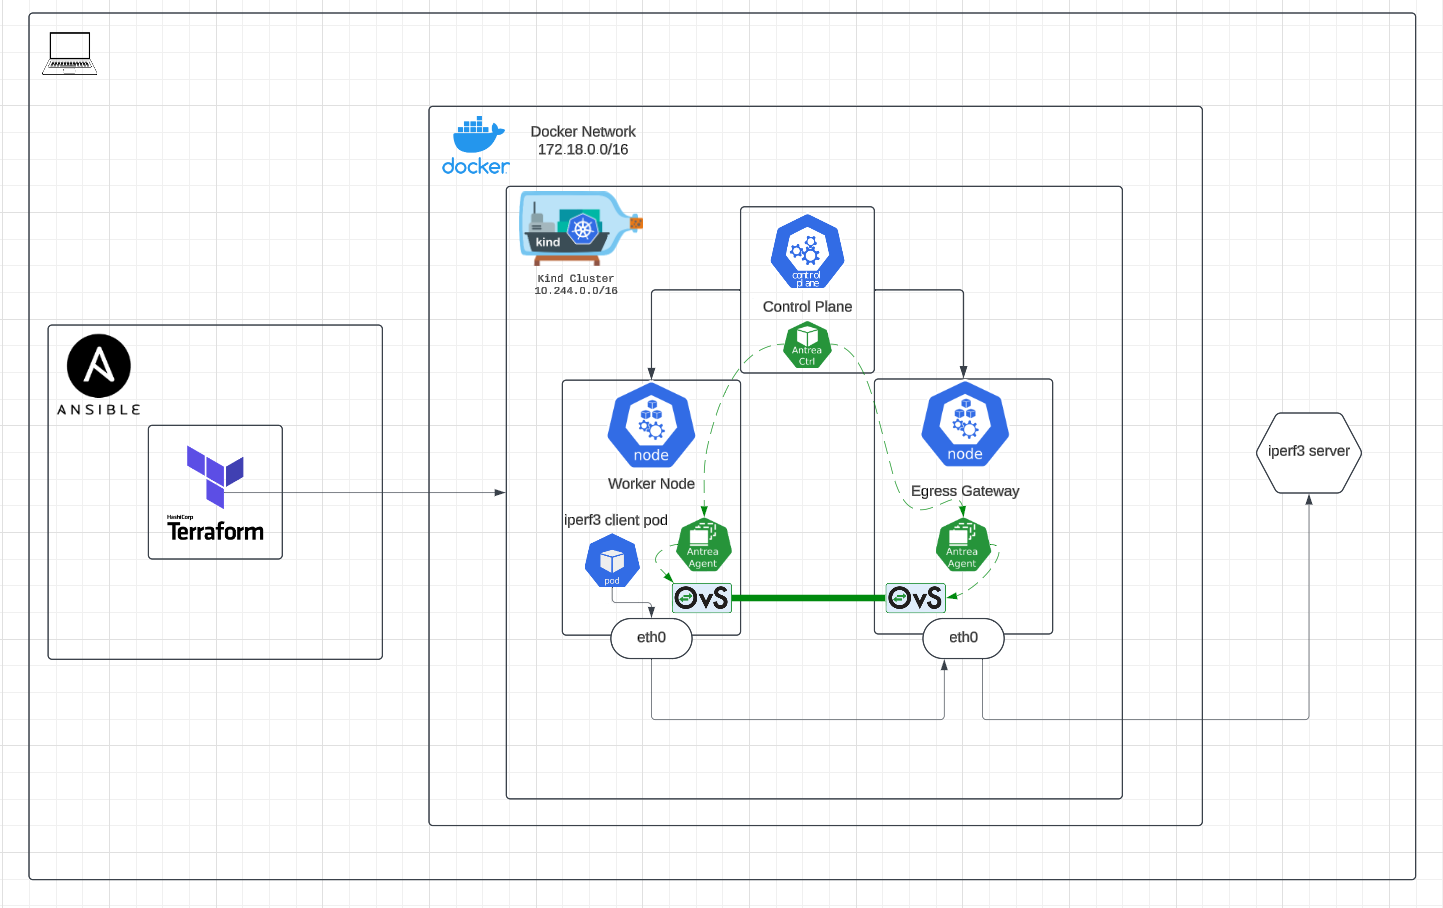
\includegraphics[width=1\columnwidth]{images/antrea_egress_gatateway_cluster.png}
  \caption{Antrea Egress Scenario infrastructure \cite{AntreaDocs}\cite{NGINX}.}
  \label{fig:antreaEgressScenarioArch}
\end{figure}

The Kubernetes cluster, as shown in Figure~\ref{fig:antreaEgressScenarioArch}, is provisioned on a personal computer using Kind and configured with Ansible and Terraform. The cluster consists of three nodes: a control plane, a worker node, and an egress gateway, all of which are part of the Docker network. When the role terraform\_run\_egress\_iperf starts execution and the created Iperf3 pod is ready, the test begins. The client, using the TCP protocol, sends data to the server (outside the cluster), which is routed through the egress gateway. The Iperf3 server detects that the traffic is coming from the egress gateway node (it sees the IP address of the egress gateway node as the source), because the traffic from the pod is SNATed.The Iperf3 client sends data packets using the TCP protocol, and after receiving acknowledgment from the server, the networking metrics are stored in memory. At the end of the test, a JSON file containing the gathered data is saved inside the pod. This file is saved on a volume shared with the host (personal laptop), ensuring that the data remains accessible after the test ends and the pod is terminated. Meanwhile, the Node Exporter continuously scrapes the metrics, which are pulled by Prometheus into its database. After the measurement is complete, the unformatted data is downloaded from Prometheus and saved as a CSV file. 

\begin{figure}[H]
  \centering
  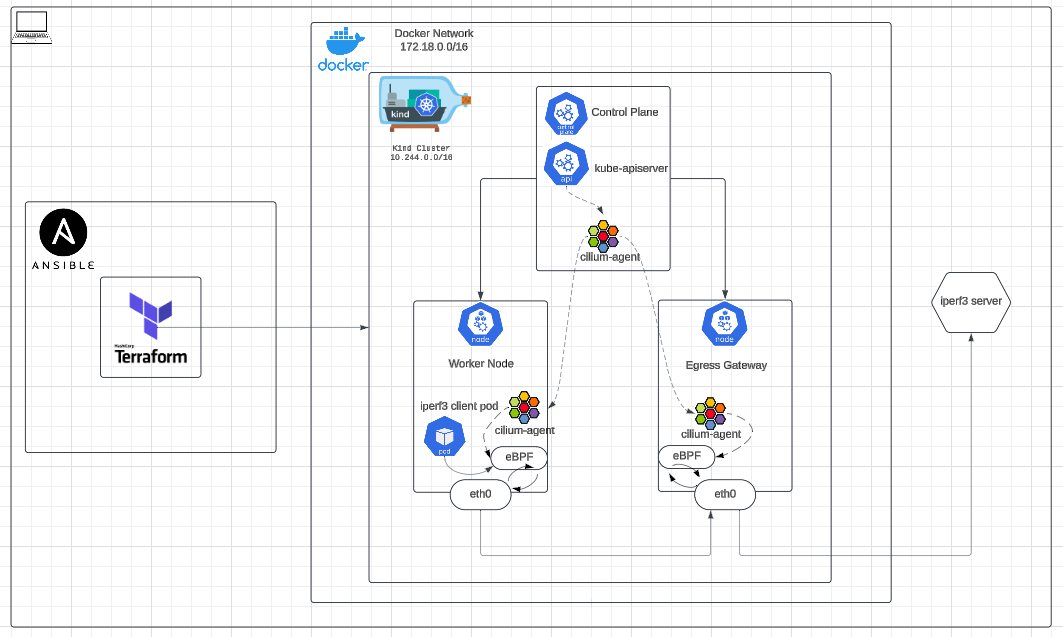
\includegraphics[width=1\columnwidth]{images/cilium_egress_gatateway_cluster.png}
  \caption{Cilium Egress Scenario infrastructure \cite{CiliumDocs}.}
  \label{fig:ciliumEgressGatewayScenarioArch}
\end{figure}

The playbook for Cilium is similar to the one used to create the egress scenario with the Antrea CNI. The Ansible roles are designed to be reusable across different playbooks. The only differences are the CNI installation, the deployment of the Egress Gateway, and in Cilium, the desired node is labeled with egress-node=true \cite{CiliumDocs}. The infrastructure can be seen in Figure~\ref{fig:ciliumEgressGatewayScenarioArch}. The Iperf3 pod starts generating traffic, which is encapsulated and sent to the egress gateway. The gateway performs IP address translation and forwards the data to the Iperf3 server outside the cluster.


%---------------------------------------------------------------------------

\section{Ingress scenario implementation}
\label{sec:ingressImpl}

The ingress scenario evaluates the CPU and memory usage of the Antrea and Cilium Container Networking Plugins while using the Gateway API to handle weighted traffic routing. The experiment involves using the Gateway API to route 40\% of incoming requests to one pod and evaluating the accuracy of traffic splitting by two different Gateway APIs. The test setup includes the K6 load testing tool running outside the Kubernetes cluster, generating traffic towards the Gateway API. The simulated traffic has four intensity levels, determined by allocating different numbers of virtual users interacting with the Gateway API. These levels are one, ten, one hundred, and one thousand virtual users. The traffic is initiated using the K6 tool, which runs inside a container on a personal computer. The network generator performs HTTP requests to the Gateway API and saves the received responses, extracting the pod name to a text file (one per line). By compiling a list of responses containing the names of two pods, the accuracy of the Gateway API traffic splitting is calculated. CPU and memory usage are monitored with a Node Exporter throughout the test and retrieved at the end of the scenario.


%---------------------------------------------------------------------------
\subsection{Cluster provisioning}
\label{sec:clusterProvisioning}

Creating a local cluster using Kind is a straightforward process, as described earlier. However, when setting up a Kubernetes cluster on Azure, the azurerm Terraform provider must be properly configured to authenticate with an Azure account. The script shown in Listing~\ref{lst:terraformScript} is responsible for creating the Kubernetes cluster in Azure Services. It is important to choose an appropriate location for the cluster, define the default node pool (including virtual machine type and node count), and remove the default CNI by setting the network\_plugin in the network\_profile to "none" if a different networking plugin is preferred \cite{AKS}.

\begin{listing}[htb]
  \centering
  \caption{Terraform Azure Kubernetes Service creation script \cite{AKS}.}
  \begin{minted}[gobble=4, frame=single, linenos, fontsize=\scriptsize]{hcl}
    resource "azurerm_resource_group" "rg" {
      location = var.resource_group_location
      name     = "rg${var.common_infix}"
    }

    resource "azurerm_kubernetes_cluster" "k8s" {
      location            = azurerm_resource_group.rg.location
      name                = "cluster${var.common_infix}"
      resource_group_name = azurerm_resource_group.rg.name
      dns_prefix          = "dns${var.common_infix}"

      identity {
        type = "SystemAssigned"
      }

      default_node_pool {
        name       = "agentpool"
        vm_size    = var.vm_type
        node_count = var.node_count
      }

      linux_profile {
        admin_username = var.username

        ssh_key {
          key_data = azapi_resource_action.ssh_public_key_gen.output.publicKey
        }
      }

      network_profile {
        network_plugin    = "none"
        load_balancer_sku = "standard"
      }
    }
  \end{minted}
  \label{lst:terraformScript}
\end{listing}


%---------------------------------------------------------------------------
\subsection{Infrastructure}
\label{sec:infra}

The process of creating an ingress scenario with Antrea CNI on Azure Kubernetes Services is fully automated showed in listing~\ref{lst:antreaIngressPlaybook}. The script provisions the infrastructure seen in Figure~\ref{fig:antreaIngressScenarioArch}. The steps in the scripts are: 


\begin{enumerate}
  \item create\_azure\_cluster -- Runs Terraform to provision infrastructure in the cloud and configures the local environment to allow kubectl to interact with the cluster.
  \item install\_antrea -- Installs Antrea CNI plugin.
  \item wait\_until\_antrea\_installed -- Waits until Antrea is installed.
  \item install\_gateway\_api\_crd -- Applies custom definition resources, Gateway, GatewayClass, HTTPRoutes etc.
  \item install\_nginx\_gateway\_fabric -- Installs NGINX Gateway Fabric using Helm and waits until is ready.
  \item deploy\_antrea\_ingress\_scenario -- Deploys the ingress scenario (echo pods and Gateway API) using Terraform.
  \item monitoring -- Enables monitoring with Node Exporter and Prometheus.
  \item register\_gateway\_api\_ip -- Registers the IP address of the Gateway API for the K6 tool.
  \item run\_k6 -- Creates a container with K6, which generates HTTP traffic accessing Gateway API.
  \item scrap\_prometheus\_data -- Downloads data about CPU and memory utilization.
\end{enumerate}

\begin{listing}[H]
  \centering
  \caption{Ansible playbook used to deploy Antrea with Gateway API \cite{AnsibleDocs}.}
  \begin{minted}[gobble=4, frame=single, linenos, fontsize=\scriptsize]{yaml}
    - name: Create antrea ingres scenario with gateway api
      hosts: "{{ target | default('localhost') }}"
      vars_files:
        - ./vars/antrea.yml
        - ./vars/cloud.yml
        - ./vars/common.yml
        - ./vars/traffic_splitting.yml

      roles:
        - create_azure_cluster
        - install_antrea_cloud
        - wait_until_antrea_installed
        - install_gateway_crd
        - install_nginx_gateway
        - deploy_antrea_ingress_scenario
        - monitoring
        - register_gateway_api_ip
        - run_k6
        - scrap_prometheus_data
  \end{minted}
  \label{lst:antreaIngressPlaybook}
\end{listing}


\begin{figure}[tbh]
  \centering
  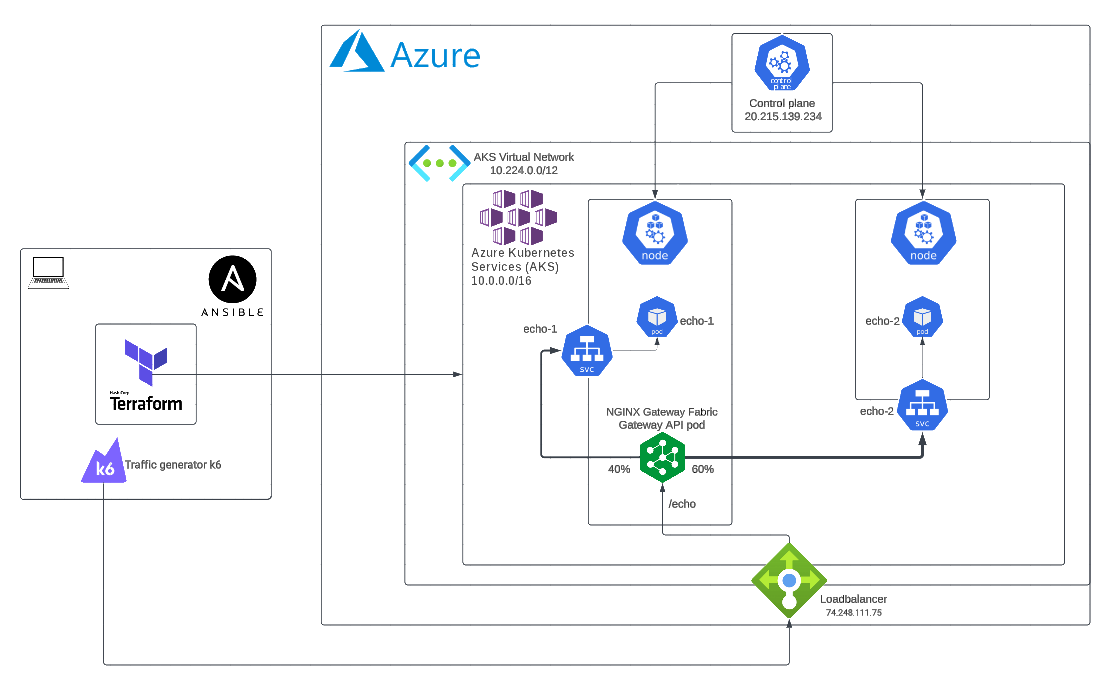
\includegraphics[width=1\columnwidth]{images/antrea_cloud_traffic_splitting.png}
  \caption{Antrea Ingress Scenario infrastructure \cite{K6}\cite{NGINX}.}
  \label{fig:antreaIngressScenarioArch}
\end{figure}

Figure~\ref{fig:antreaIngressScenarioArch} shows the cluster created using the script from Listing~\ref{lst:antreaIngressPlaybook}. In the cloud environment, the NGINX Gateway API pod is located on one of the nodes, which also runs the echo pod. Communication between the two pods within the node occurs via the Open vSwitch (OvS) bridge \cite{AntreaDocs}. In the local infrastructure, the gateway is forced to be deployed on the control plane node, so it uses Node-to-Node communication when routing traffic. Since Cilium uses the Gateway API, which does not run in a pod, the resource utilization is distributed between both nodes to Envoy.

%---------------------------------------------------------------------------


\begin{figure}[H]
  \centering
  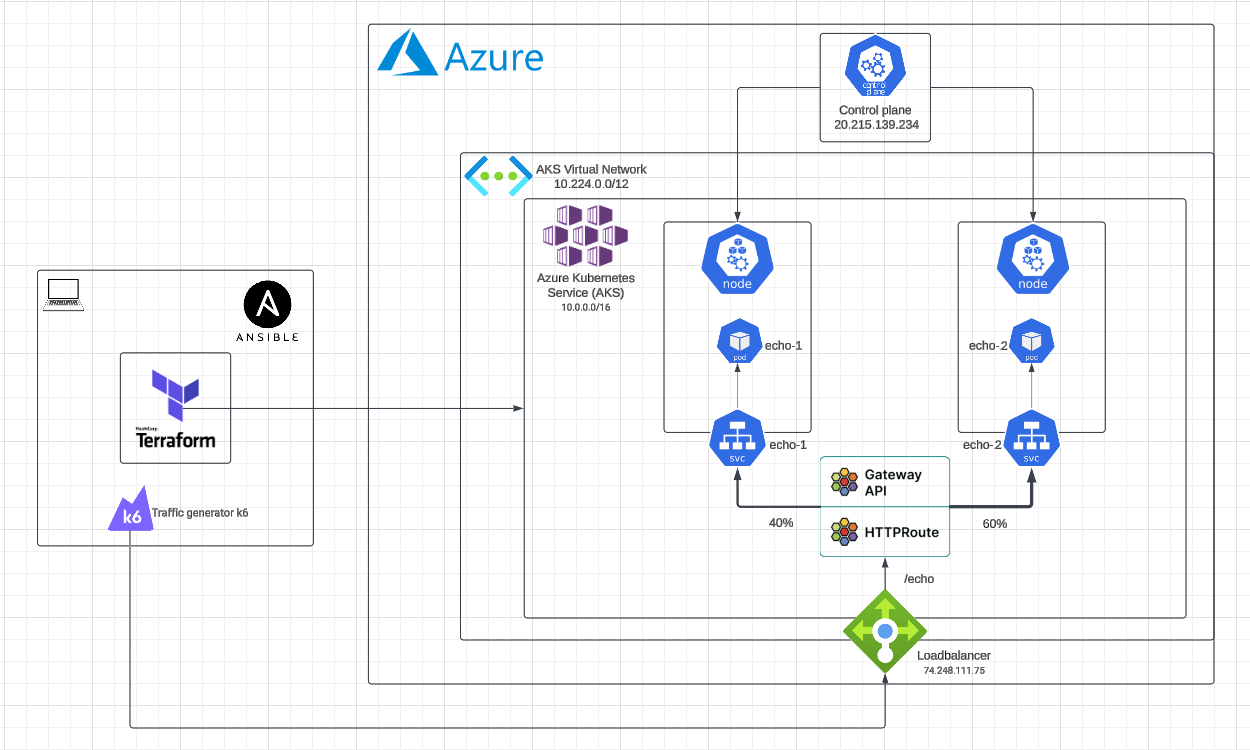
\includegraphics[width=1\columnwidth]{images/cilium_cloud_traffic_splitting.png}
  \caption{Cilium Ingress Scenario infrastructure \cite{CiliumDocs}\cite{CiliumUseCases}.}
  \label{fig:ciliumIngressScenarioArch}
\end{figure}

Both test cases, shown in Figures~\ref{fig:antreaIngressScenarioArch} and~\ref{fig:ciliumIngressScenarioArch}, consist of two nodes, each running echo pods. The pods host an application designed to return their pod name when a request is made to the "/echo" endpoint. The Grafana K6 tool sends requests to the exposed Gateway API IP address and, in return, logs which pod responded to the request. This information is used to calculate the accuracy of traffic weighting in both configurations. The load balancer shown at the bottom of the figures exposes the Gateway API to a public IP address so that the K6 client, located on a personal computer, can perform the requests. It does not split the traffic; that is done by the Gateway API.

The ingress scenario using the Cilium CNI plugin does not require the installation of NGINX Gateway Fabric, as it utilizes its own built-in implementation.

%---------------------------------------------------------------------------

\subsection{The differences between cloud and local runs}
\label{sec:diff}

\subsubsection{Control plane}
\label{sec:cplaneDiff}

In the local environment, the control plane node is created in the same way as the worker nodes, running as a container. However, when using NGINX with the Antrea CNI, the NGINX Gateway Fabric pod is deployed on a separate control plane node. This setup allows the routing of traffic between two different nodes, ensuring that traffic always exits the node. In contrast, when using AKS (Azure Kubernetes Service), the control plane is not part of the node pool; it is a separate managed service outside the node pool, providing a clearer separation between the control plane and worker nodes. This architectural difference can affect the measurements (compared to the local stack), as resource utilization of the control plane node is not gathered.

\subsubsection{Client traffic generator}
\label{sec:clientServerDiff}

In the cloud setup, the client running on a personal computer generates HTTP requests to the public Gateway API IP address exposed by Azure Cloud. Resource utilization within the cluster is exclusive to the cluster itself, not the client. However, when running the local stack, the client is part of the laptop on which the cluster is running, which could influence the measurements.

\chapter{Performance comparison}
\label{cha:performCompare}

In this chapter, the test results for both ingress and egress scenarios will be presented and analyzed, focusing on comparing CPU and memory usage in each case. For the ingress scenario, the analysis will cover weighted traffic splitting through the Gateway API, evaluating its impact on resource utilization and the accuracy of traffic distribution. The test was conducted sixteen times, each lasting only two minutes, because during traffic generation by a thousand virtual users, the logs reached up to half a million lines. For the egress scenario, the evaluation will include traffic routing through an egress gateway, comparing throughput and round-trip time. The egress test was conducted eight times, each lasting twelve minutes. The results will highlight differences in resource efficiency and networking performance between the Antrea and Cilium CNI plugins, identifying which CNI offers better optimization for these scenarios.


\section{Egress Scenario}
\label{sec:egressComparison}

In this section, a comparison of the Antrea and Cilium CNI plugins is presented, focusing on differences in networking metrics and resource consumption when using an egress gateway and when not.

\subsubsection{Resource consumption}
\label{sec:egressResoureComsumption}



Figures~\ref{fig:cpu_avg} and~\ref{fig:memory_avg} show that resource utilization is lower when using an egress gateway compared to scenarios without redirecting outgoing packets via an additional node. This could be because all traffic management (routing table, NAT rules, and maps) is offloaded to the egress gateway. In this setup, the node running the Iperf3 pod does not need to evaluate routing decisions. Instead, it simply forwards all traffic to the egress gateway (where address translation occurs), allowing the node to allocate more CPU resources to the pod running the Iperf3 client. Without the egress gateway, the individual nodes are responsible for handling more operations, which can lead to higher resource usage. Figures~\ref{fig:cpu_all} and~\ref{fig:memory_all} show the results of all eight runs across the four test cases. The sixth run in Figure~\ref{fig:cpu_all}, during the Cilium egress gateway case, is an outlier and was excluded from the calculation of the total average (using a truncated mean). Overall, CPU usage is lower when the cluster uses Antrea networking. As for memory usage, Antrea consumes 10\% less memory when using the egress gateway and up to almost 20\% less when not using an additional node, compared to Cilium. 

\begin{figure}[H]
    \centering
    \begin{subfigure}[b]{1\textwidth}
        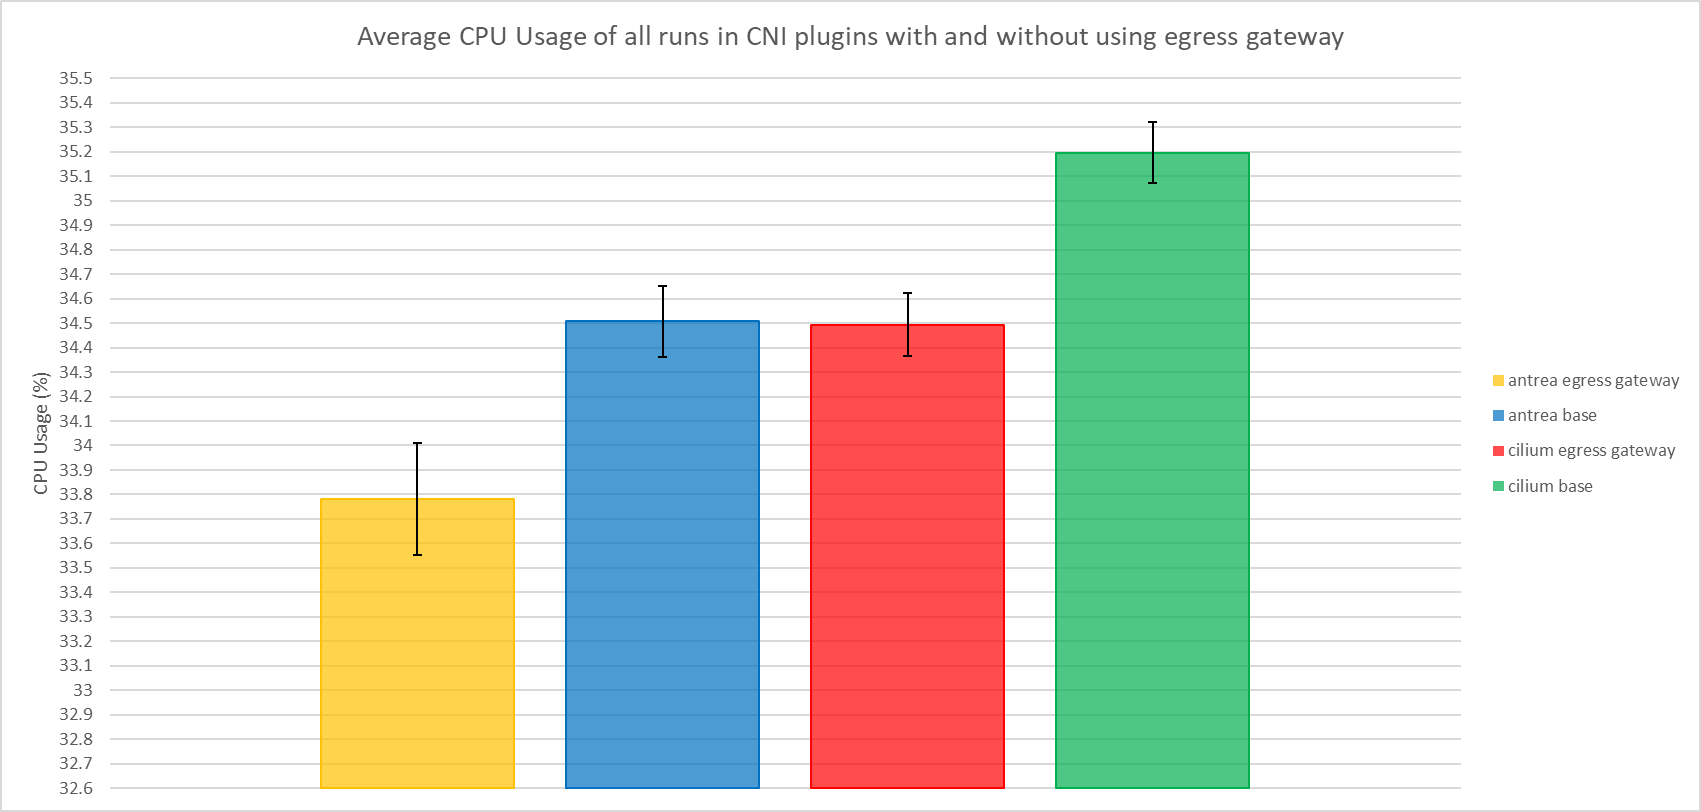
\includegraphics[width=\textwidth]{plots/egress/cpu_total_average.png}
        \caption{}
        \label{fig:cpu_avg}
    \end{subfigure}
    \begin{subfigure}[b]{1\textwidth}
        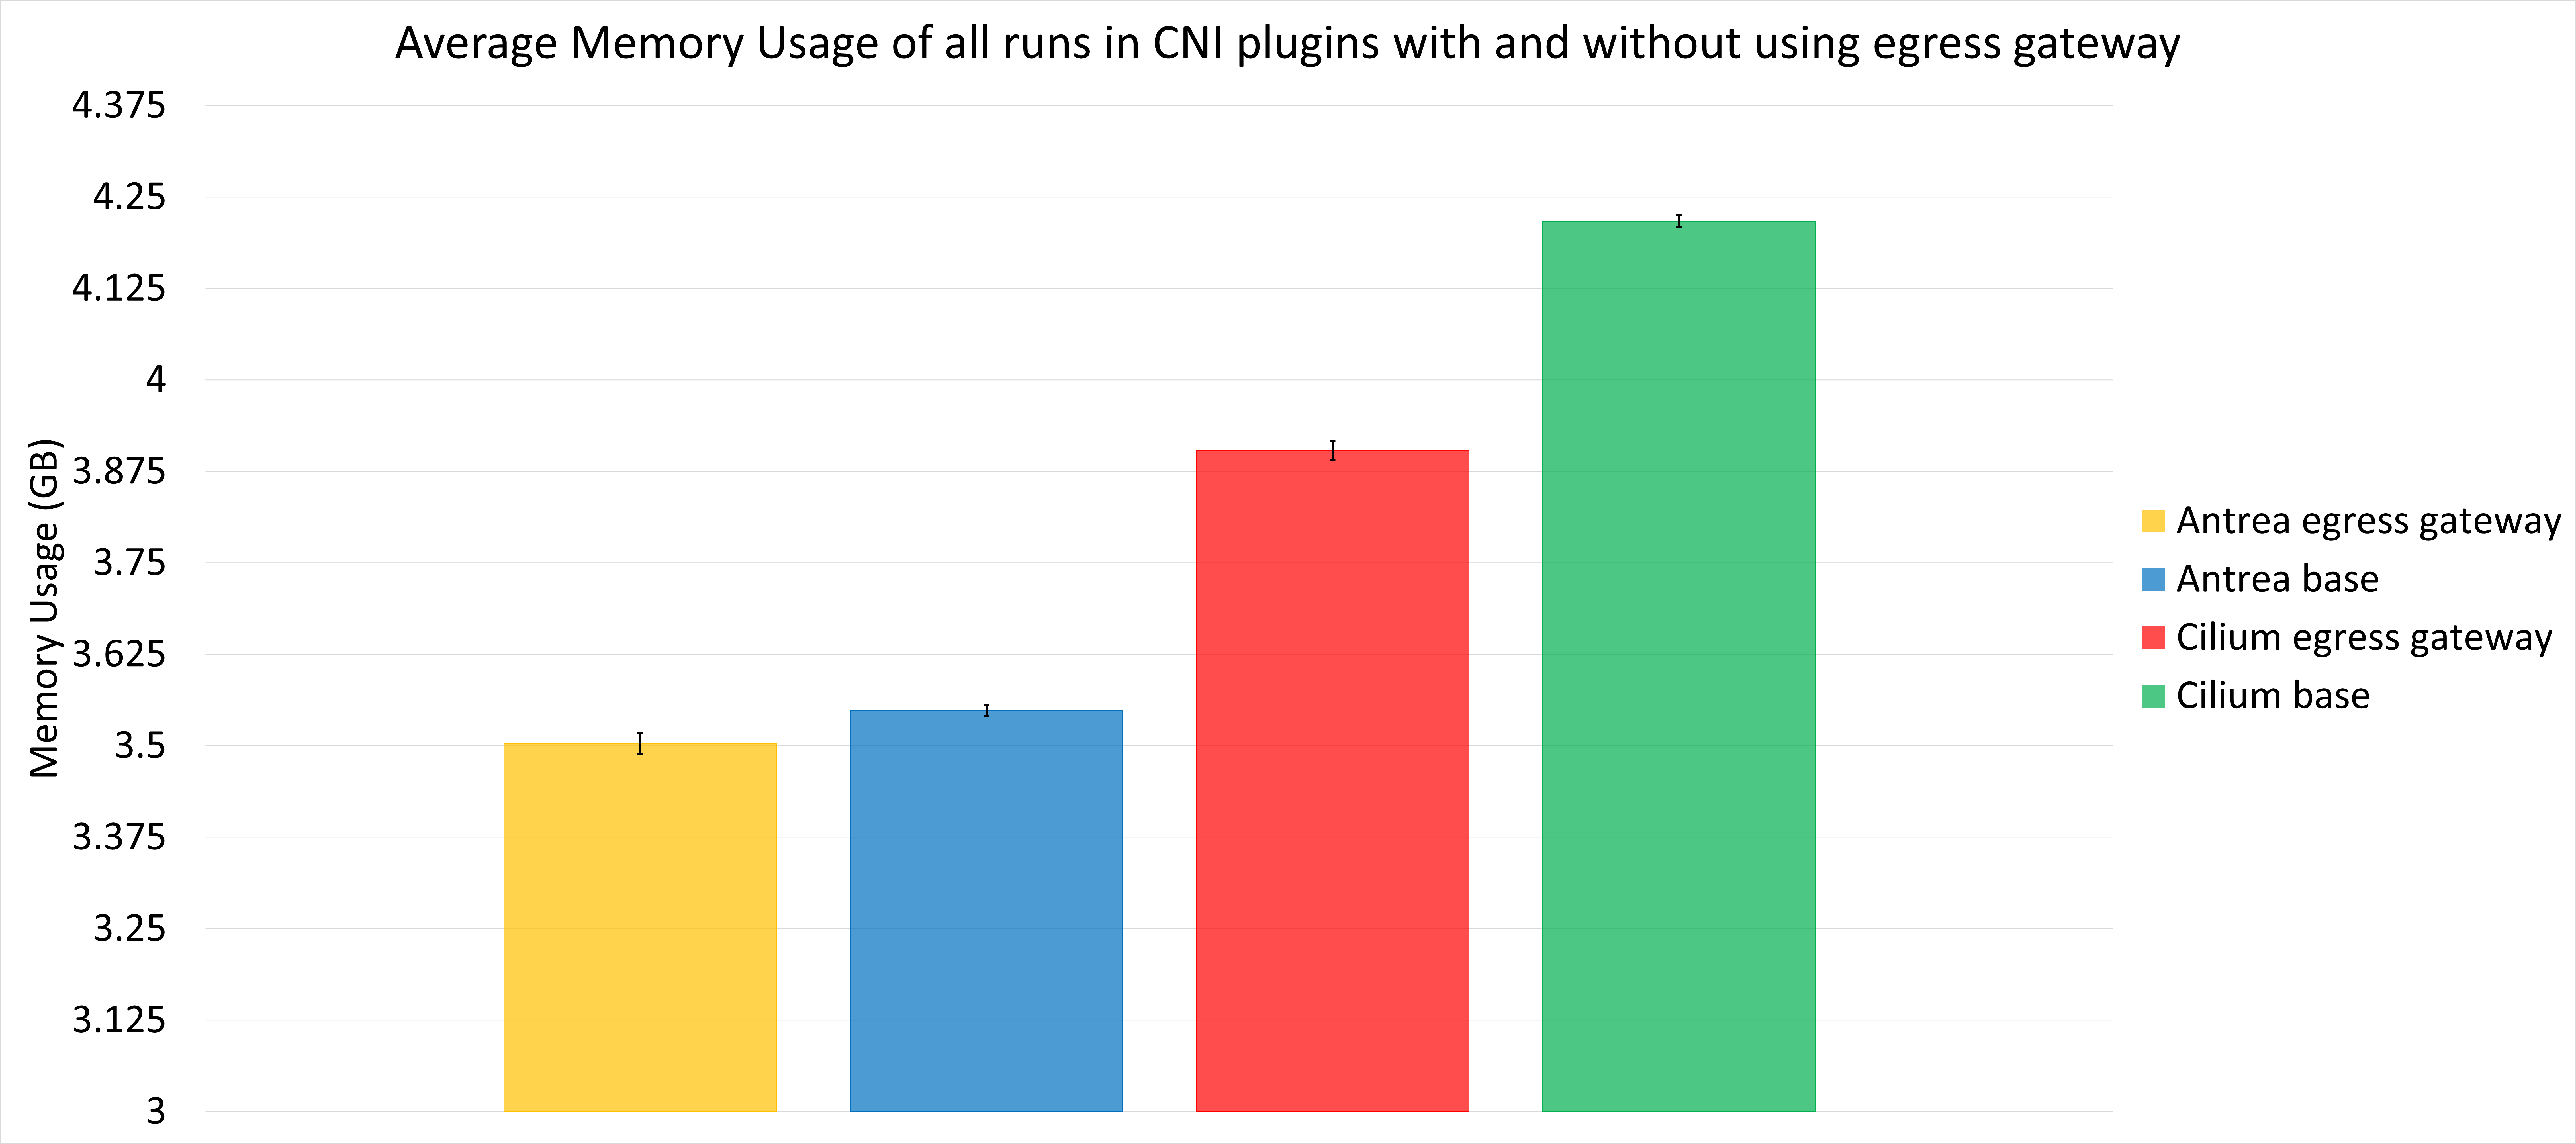
\includegraphics[width=\textwidth]{plots/egress/memory_total_average.png}
        \caption{}
        \label{fig:memory_avg}
    \end{subfigure}
    
    \caption{Average resource consumption in egress scenario, (a) CPU, (b) Memory}
    \label{fig:res_avg}
\end{figure}


\begin{figure}[H]
    \centering
    \begin{subfigure}[b]{1\textwidth}
        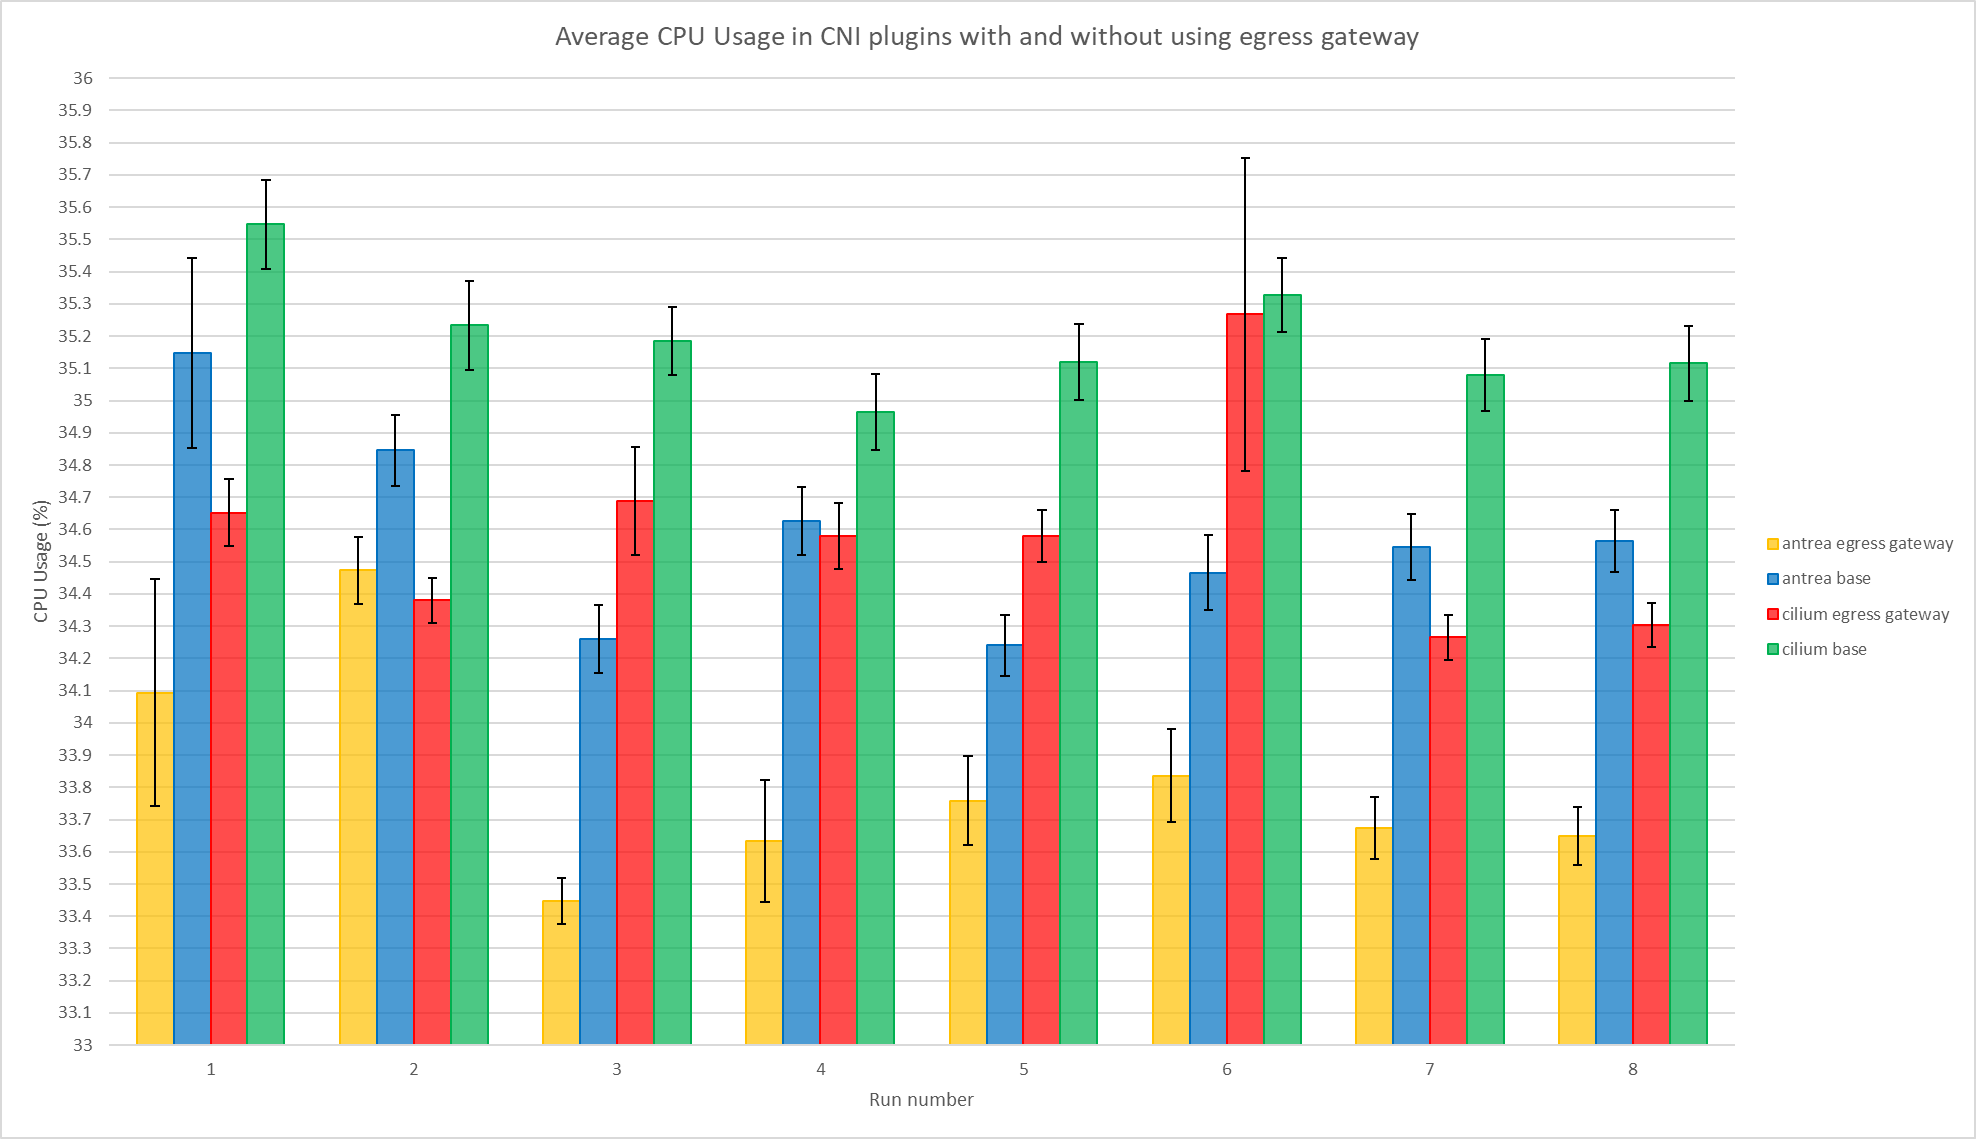
\includegraphics[width=\textwidth]{plots/egress/cpu_all.png}
        \caption{}
        \label{fig:cpu_all}
    \end{subfigure}
    \begin{subfigure}[b]{1\textwidth}
        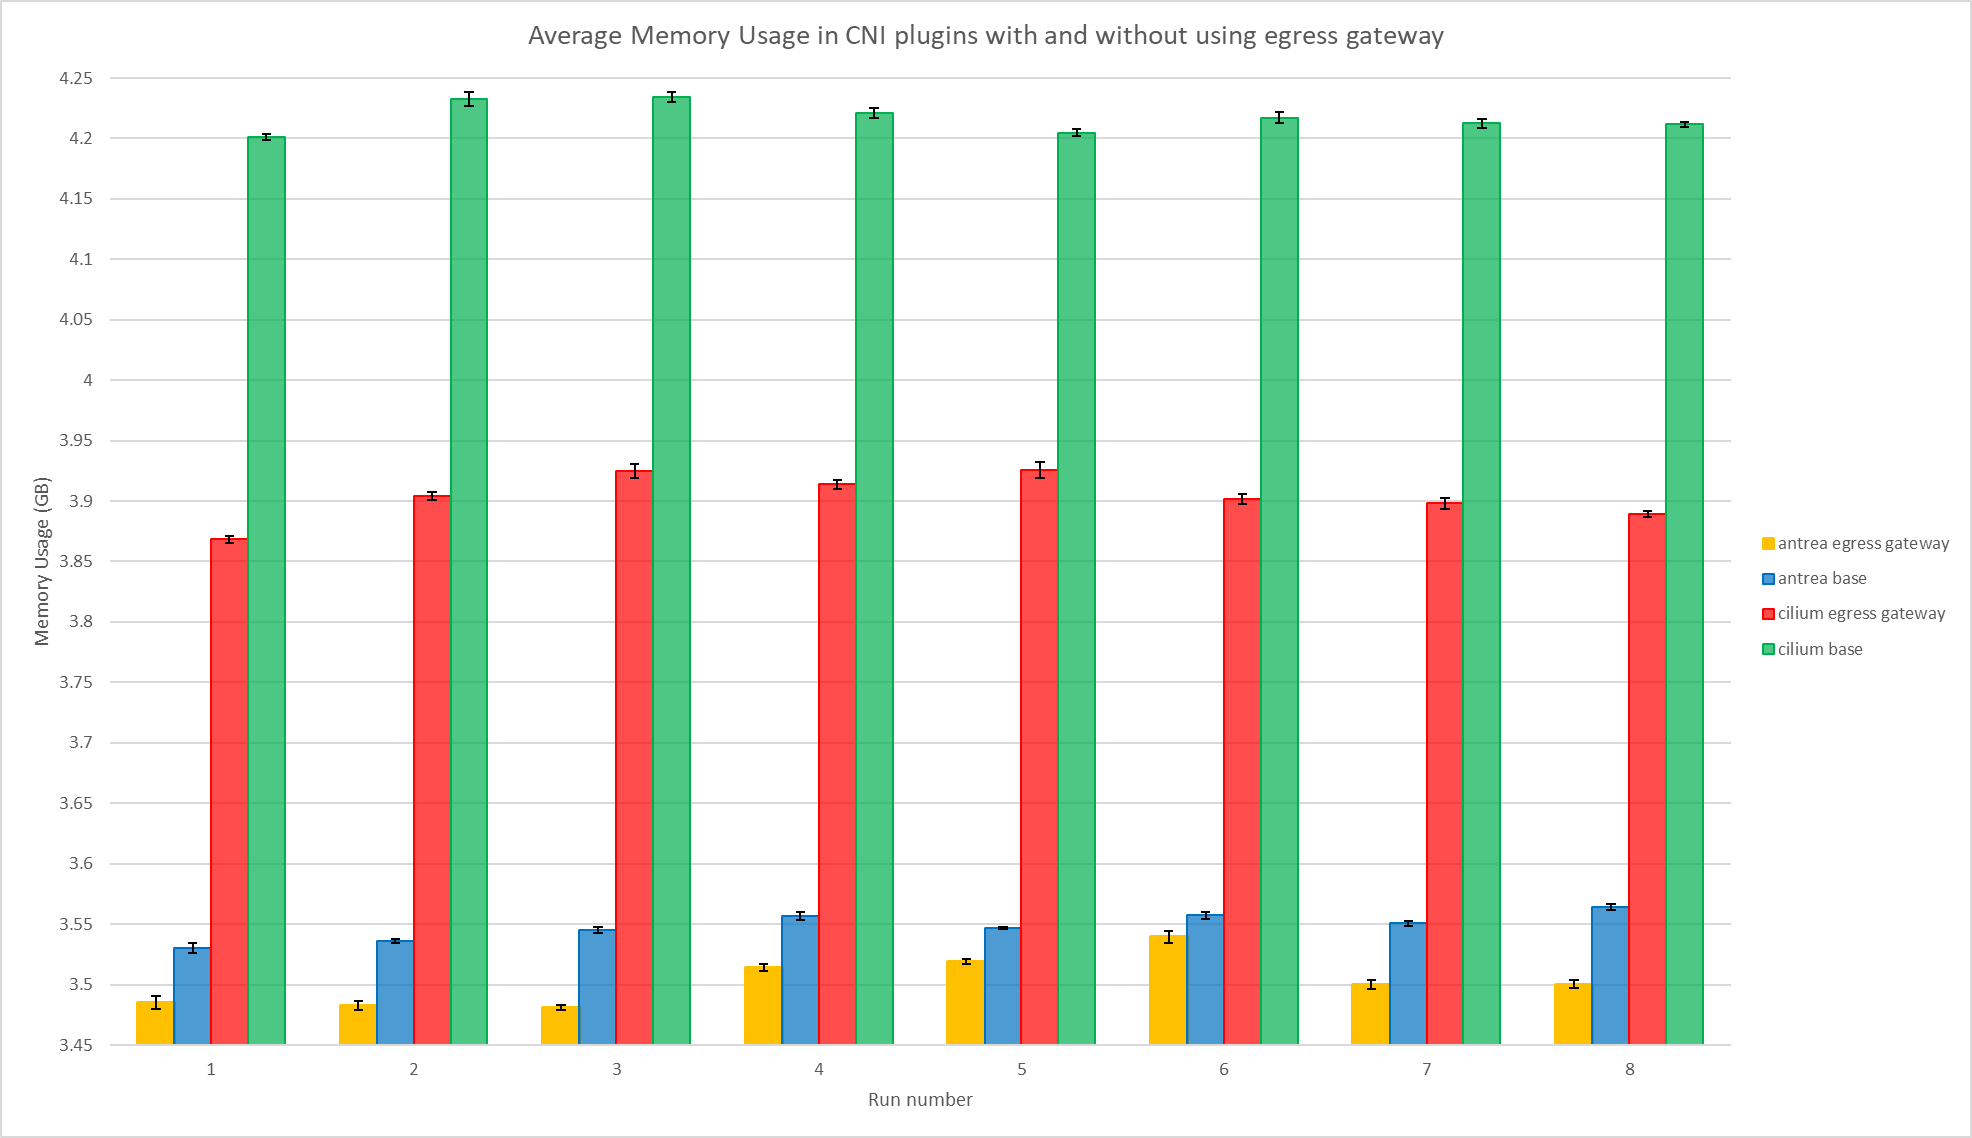
\includegraphics[width=\textwidth]{plots/egress/memory_all.png}
        \caption{}
        \label{fig:memory_all}
    \end{subfigure}
    
    \caption{Average resource consumption in egress scenario in each run, (a) CPU, (b) Memory}
    \label{fig:res_all}
\end{figure}


These figures compare the average CPU and memory usage between Cilium and Antrea CNI across all eight runs. Demonstrates how both container network interface plugins perform under the same test conditions, helping to evaluate which plugin consumes fewer resources. In only the second run did Antrea not use less CPU than Cilium. It also highlights how using an egress gateway with each CNI plugin affects resource usage, compared to scenarios where an egress gateway is not used.



\subsubsection{Networking performance}
\label{sec:egressNetworkingPerformance}

Figures~\ref{fig:throughput_avg} and~\ref{fig:rtt_avg} provide an overall performance summary as the average of all runs. Antrea handles traffic more efficiently, with lower round-trip times, regardless of whether an egress gateway is used. The plots in~\ref{fig:throughput_all} and~\ref{fig:rtt_all} display the results of all eight runs for each test case, showing that Antrea outperforms Cilium in every single run, achieving higher throughput and lower bidirectional latency.

\begin{figure}[H]
    \centering
    \begin{subfigure}[b]{1\textwidth}
        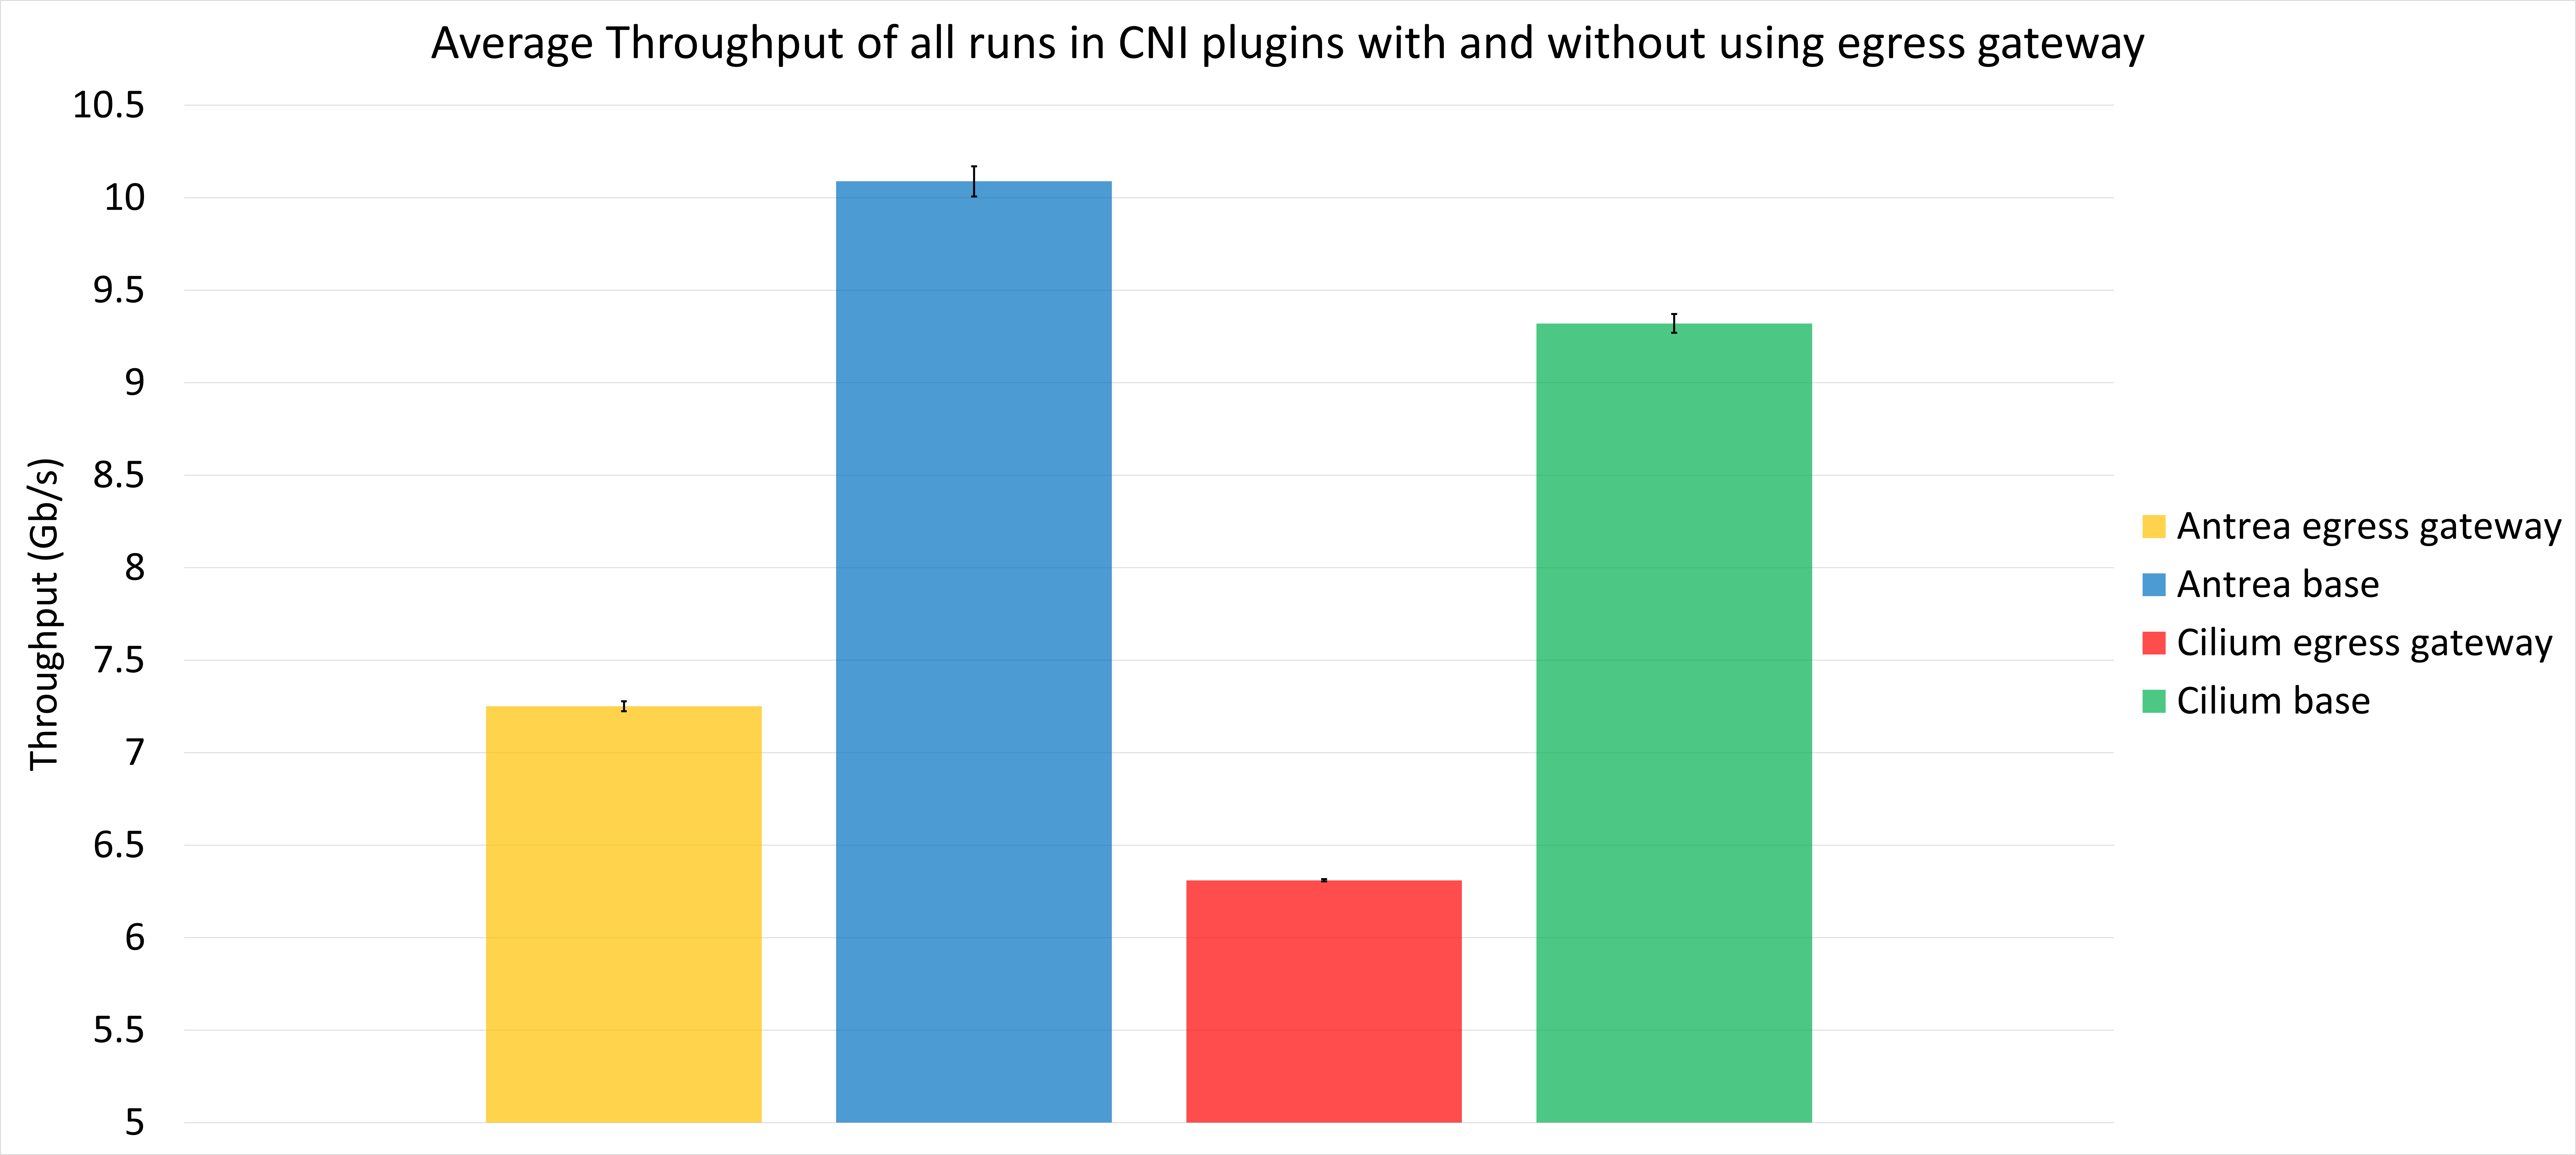
\includegraphics[width=\textwidth]{plots/egress/throughput_total_average.png}
        \caption{}
        \label{fig:throughput_avg}
    \end{subfigure}
    \begin{subfigure}[b]{1\textwidth}
        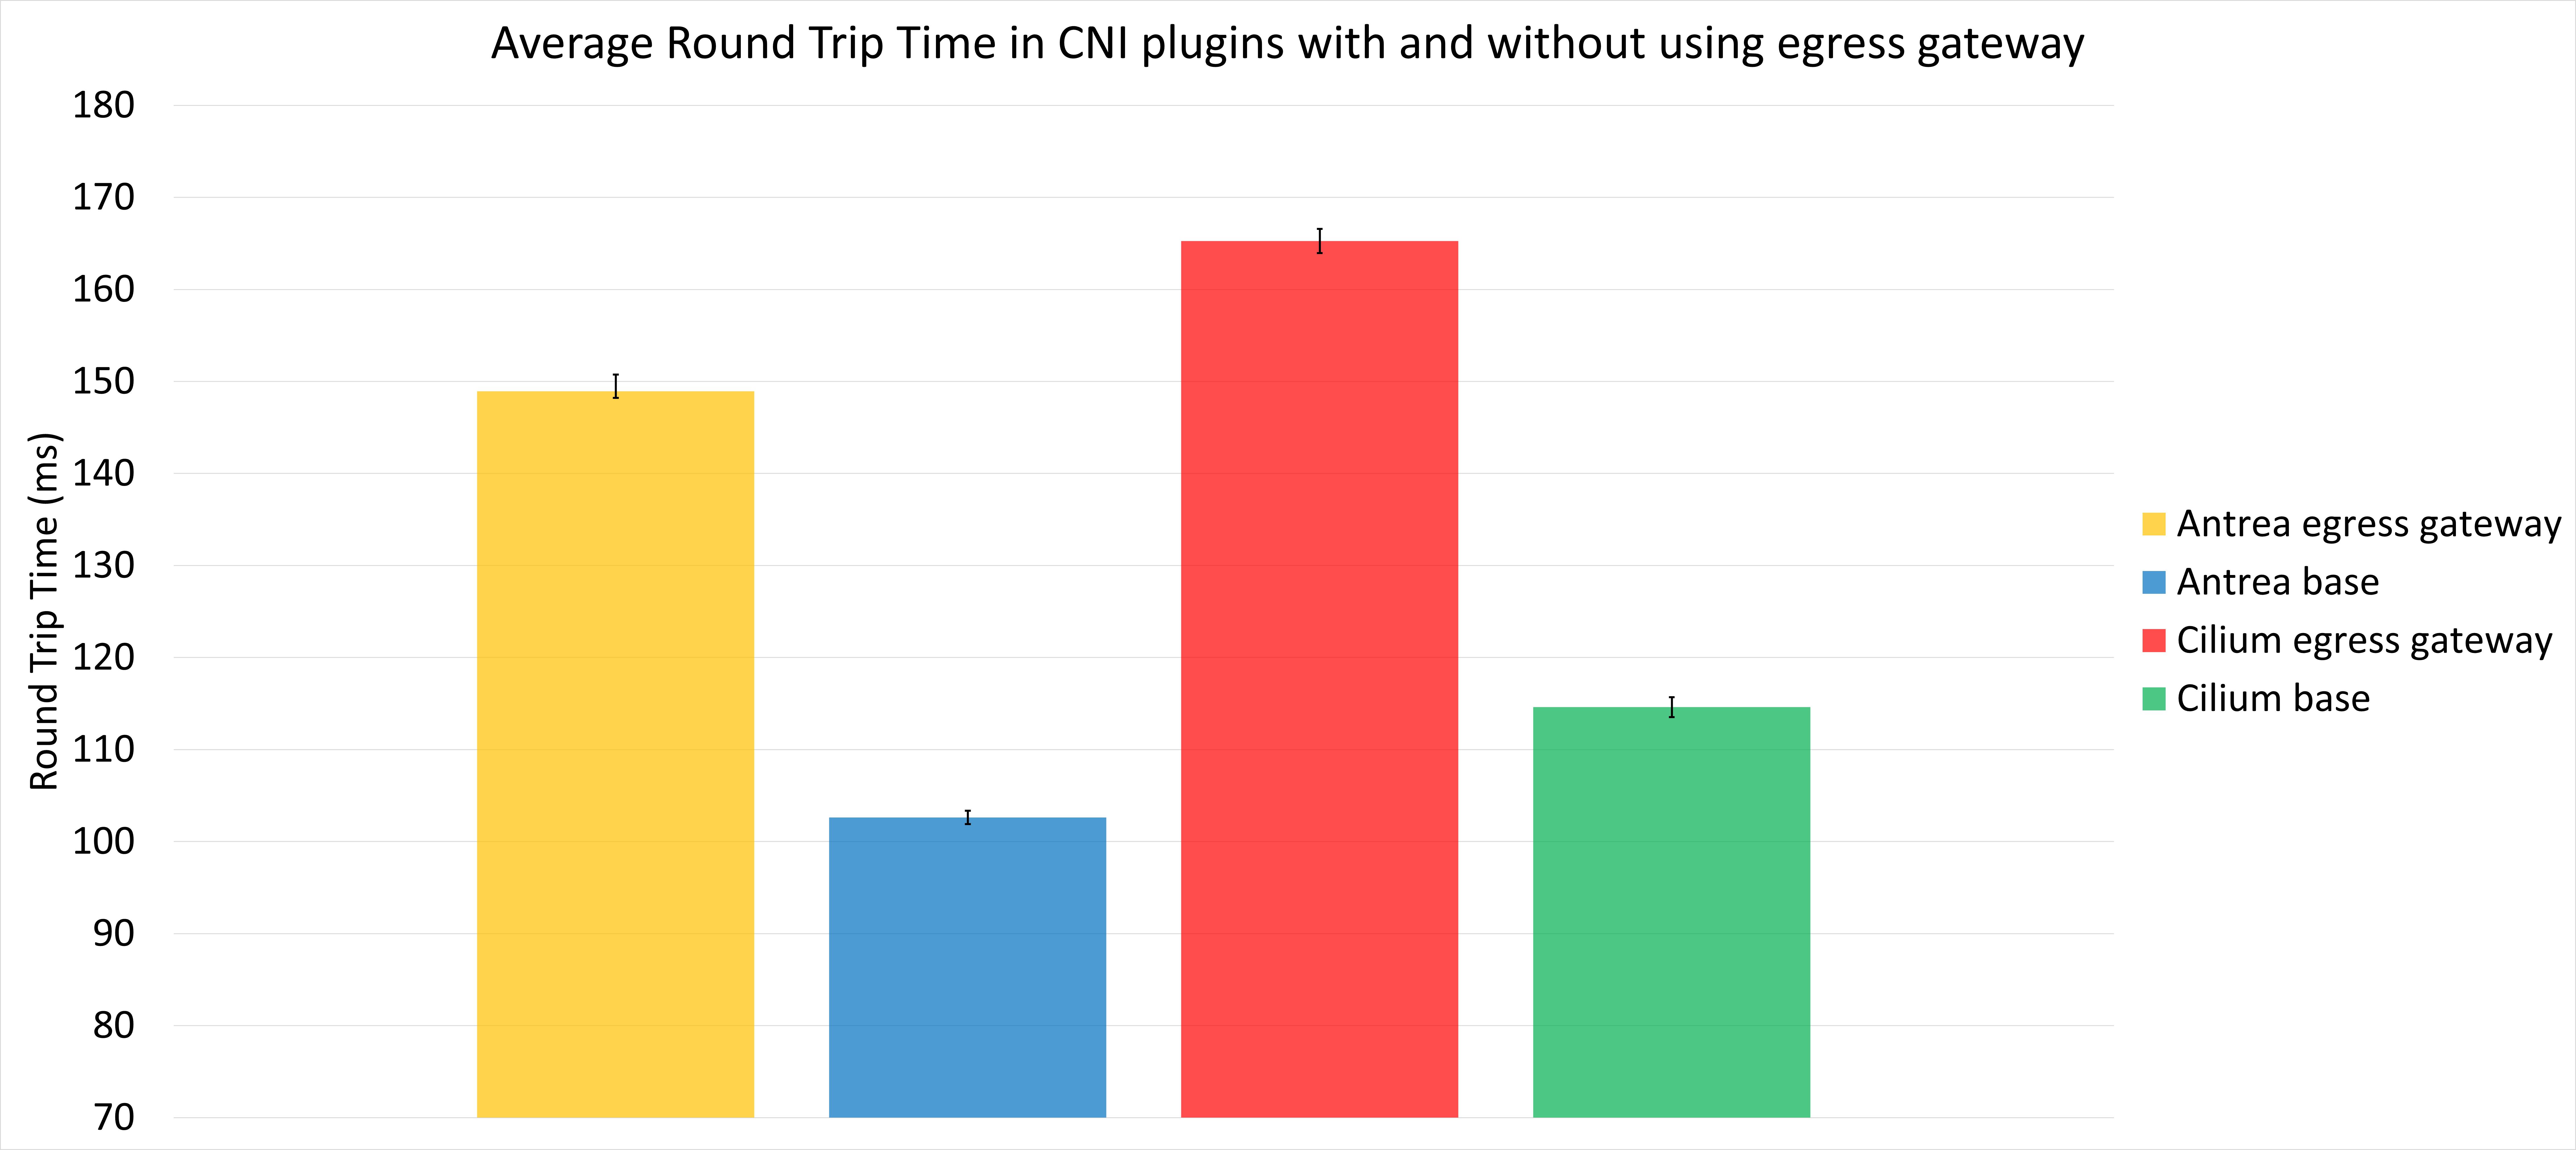
\includegraphics[width=\textwidth]{plots/egress/rtt_total_average.png}
        \caption{}
        \label{fig:rtt_avg}
    \end{subfigure}
    
    \caption{Average networking performance in egress scenario, (a) Throughput, (b) Round Trip Time}
    \label{fig:networking_avg}
\end{figure}

\begin{figure}[H]
    \centering
    \begin{subfigure}[b]{1\textwidth}
        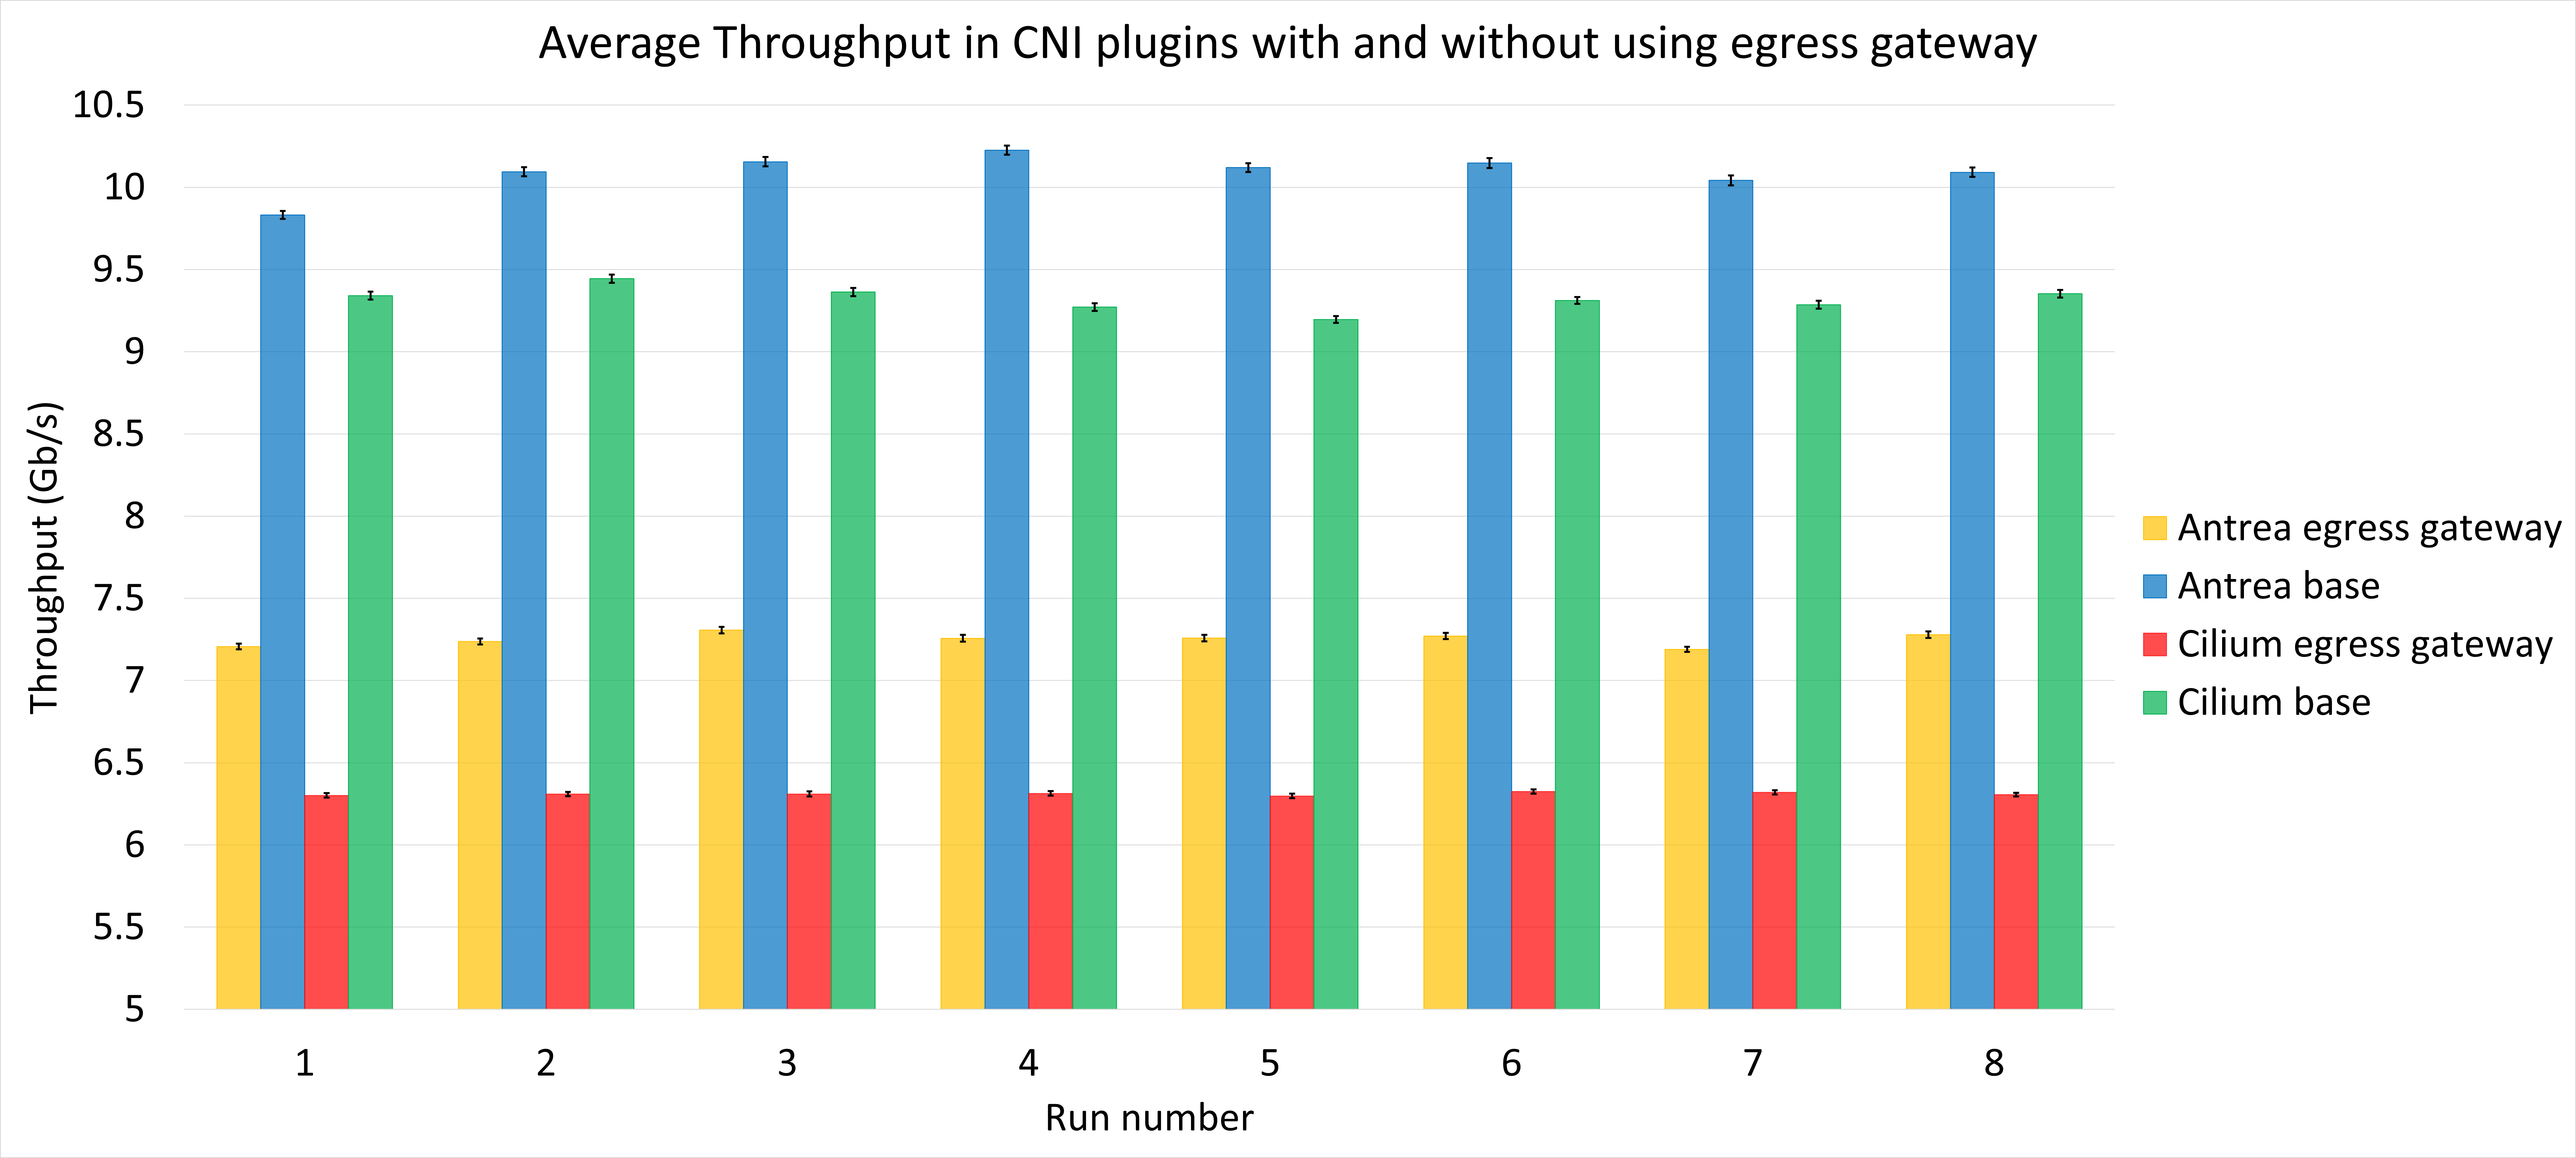
\includegraphics[width=\textwidth]{plots/egress/throughput_all.png}
        \caption{}
        \label{fig:throughput_all}
    \end{subfigure}
    \begin{subfigure}[b]{1\textwidth}
        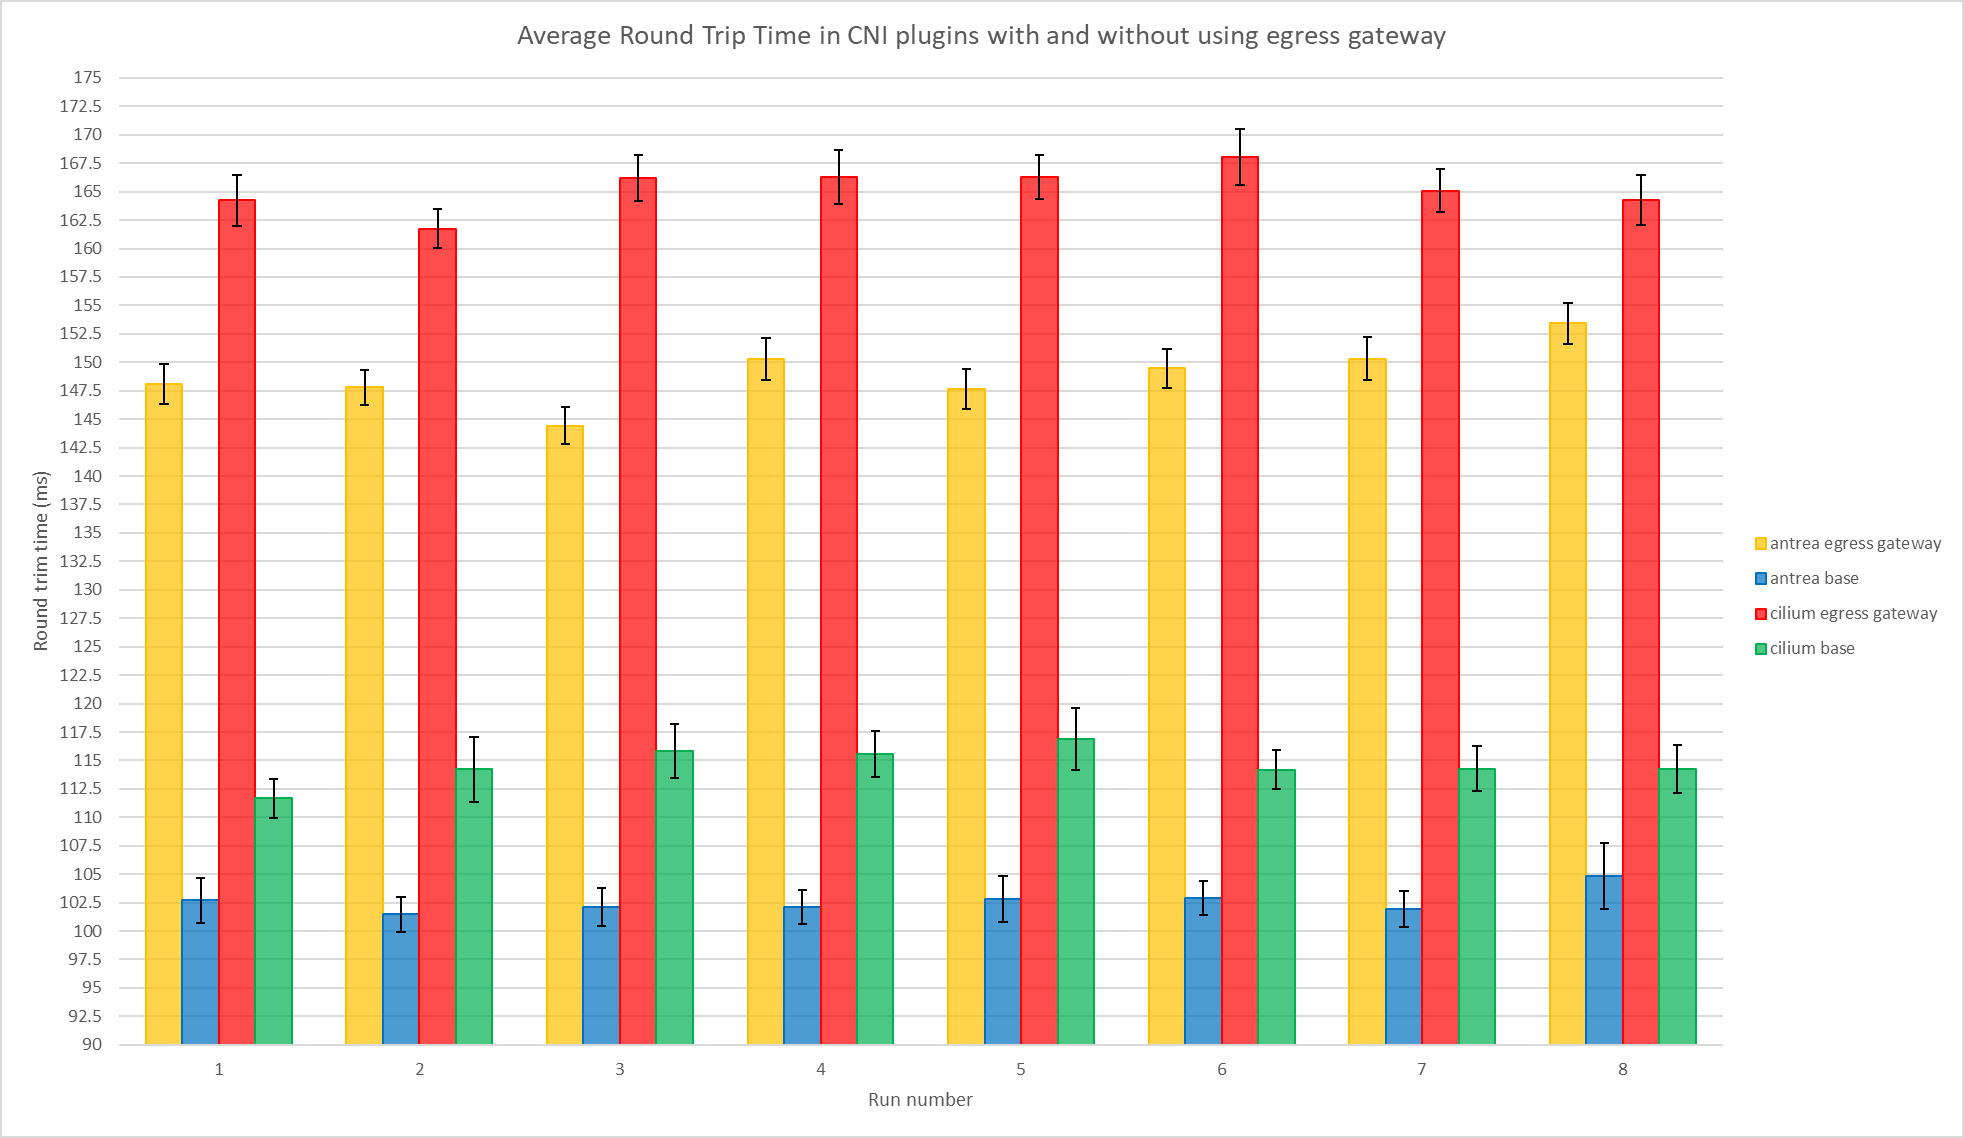
\includegraphics[width=\textwidth]{plots/egress/rtt_all.png}
        \caption{}
        \label{fig:rtt_all}
    \end{subfigure}
    
    \caption{Average networking performance in egress scenario in each run, (a) Throughput, (b) Round Trip Time}
    \label{fig:networking_avg_all}
\end{figure}




Figures~\ref{fig:throughput_all} and~\ref{fig:rtt_all} illustrate the average throughput and round-trip time across eight runs, comparing the performance of the networking plugins. Throughput with the Cilium egress gateway remains stable, hovering around 6.3 Gb/s, with tighter confidence intervals indicating greater stability. In every run, Antrea demonstrates an advantage in both data transfer rate and RTT. It also compare the performance of the CNI plugins with and without the use of an egress gateway. They highlight whether using an egress gateway is beneficial, showing significant differences in throughput and round-trip time.


This performance advantage of Antrea could be attributed to the fact that Cilium uses eBPF, which was designed for large-scale clusters. Since the current cluster consists of only a few pods, eBPF features are not fully leveraged, and Antrea's networking simplicity results in better data rates.

\section{Ingress Scenario}
\label{sec:ingressComparison}

This section presents a comparison of the Antrea and Cilium CNI plugins in ingress scenario. The tests were performed in both local and cloud environments to evaluate their performance.

\subsubsection{Resource consumption}
\label{sec:ingressResoureComsumption}


\begin{figure}[H]
    \centering
    \begin{subfigure}[b]{1\textwidth}
        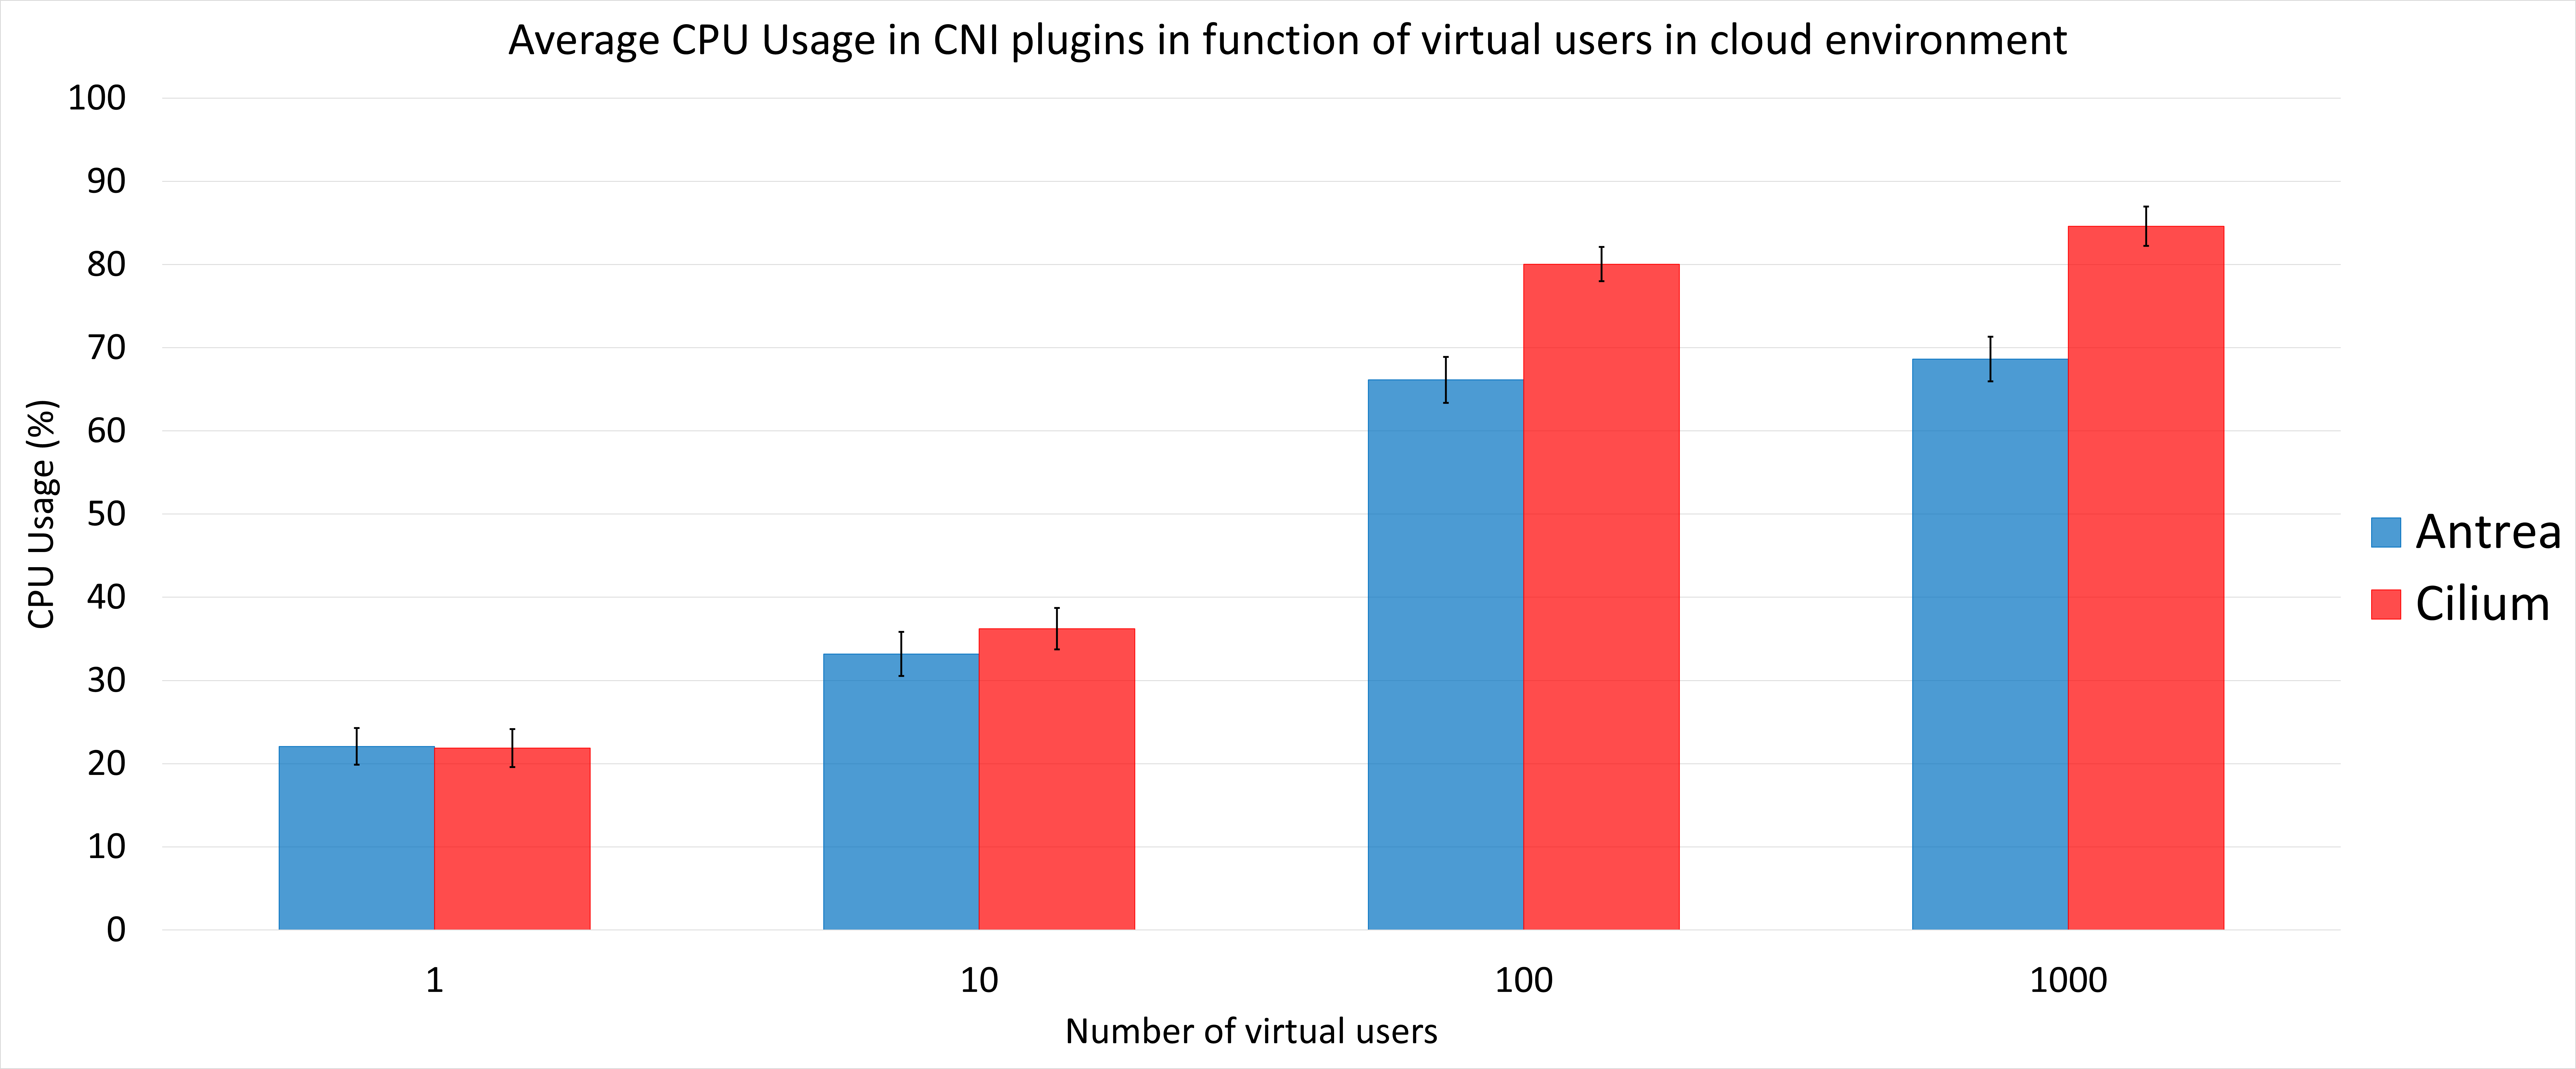
\includegraphics[width=\textwidth]{plots/traffic-splitting/cpu_cloud.png}
        \caption{}
        \label{fig:cpu_cloud_avg}
    \end{subfigure}
    \begin{subfigure}[b]{1\textwidth}
        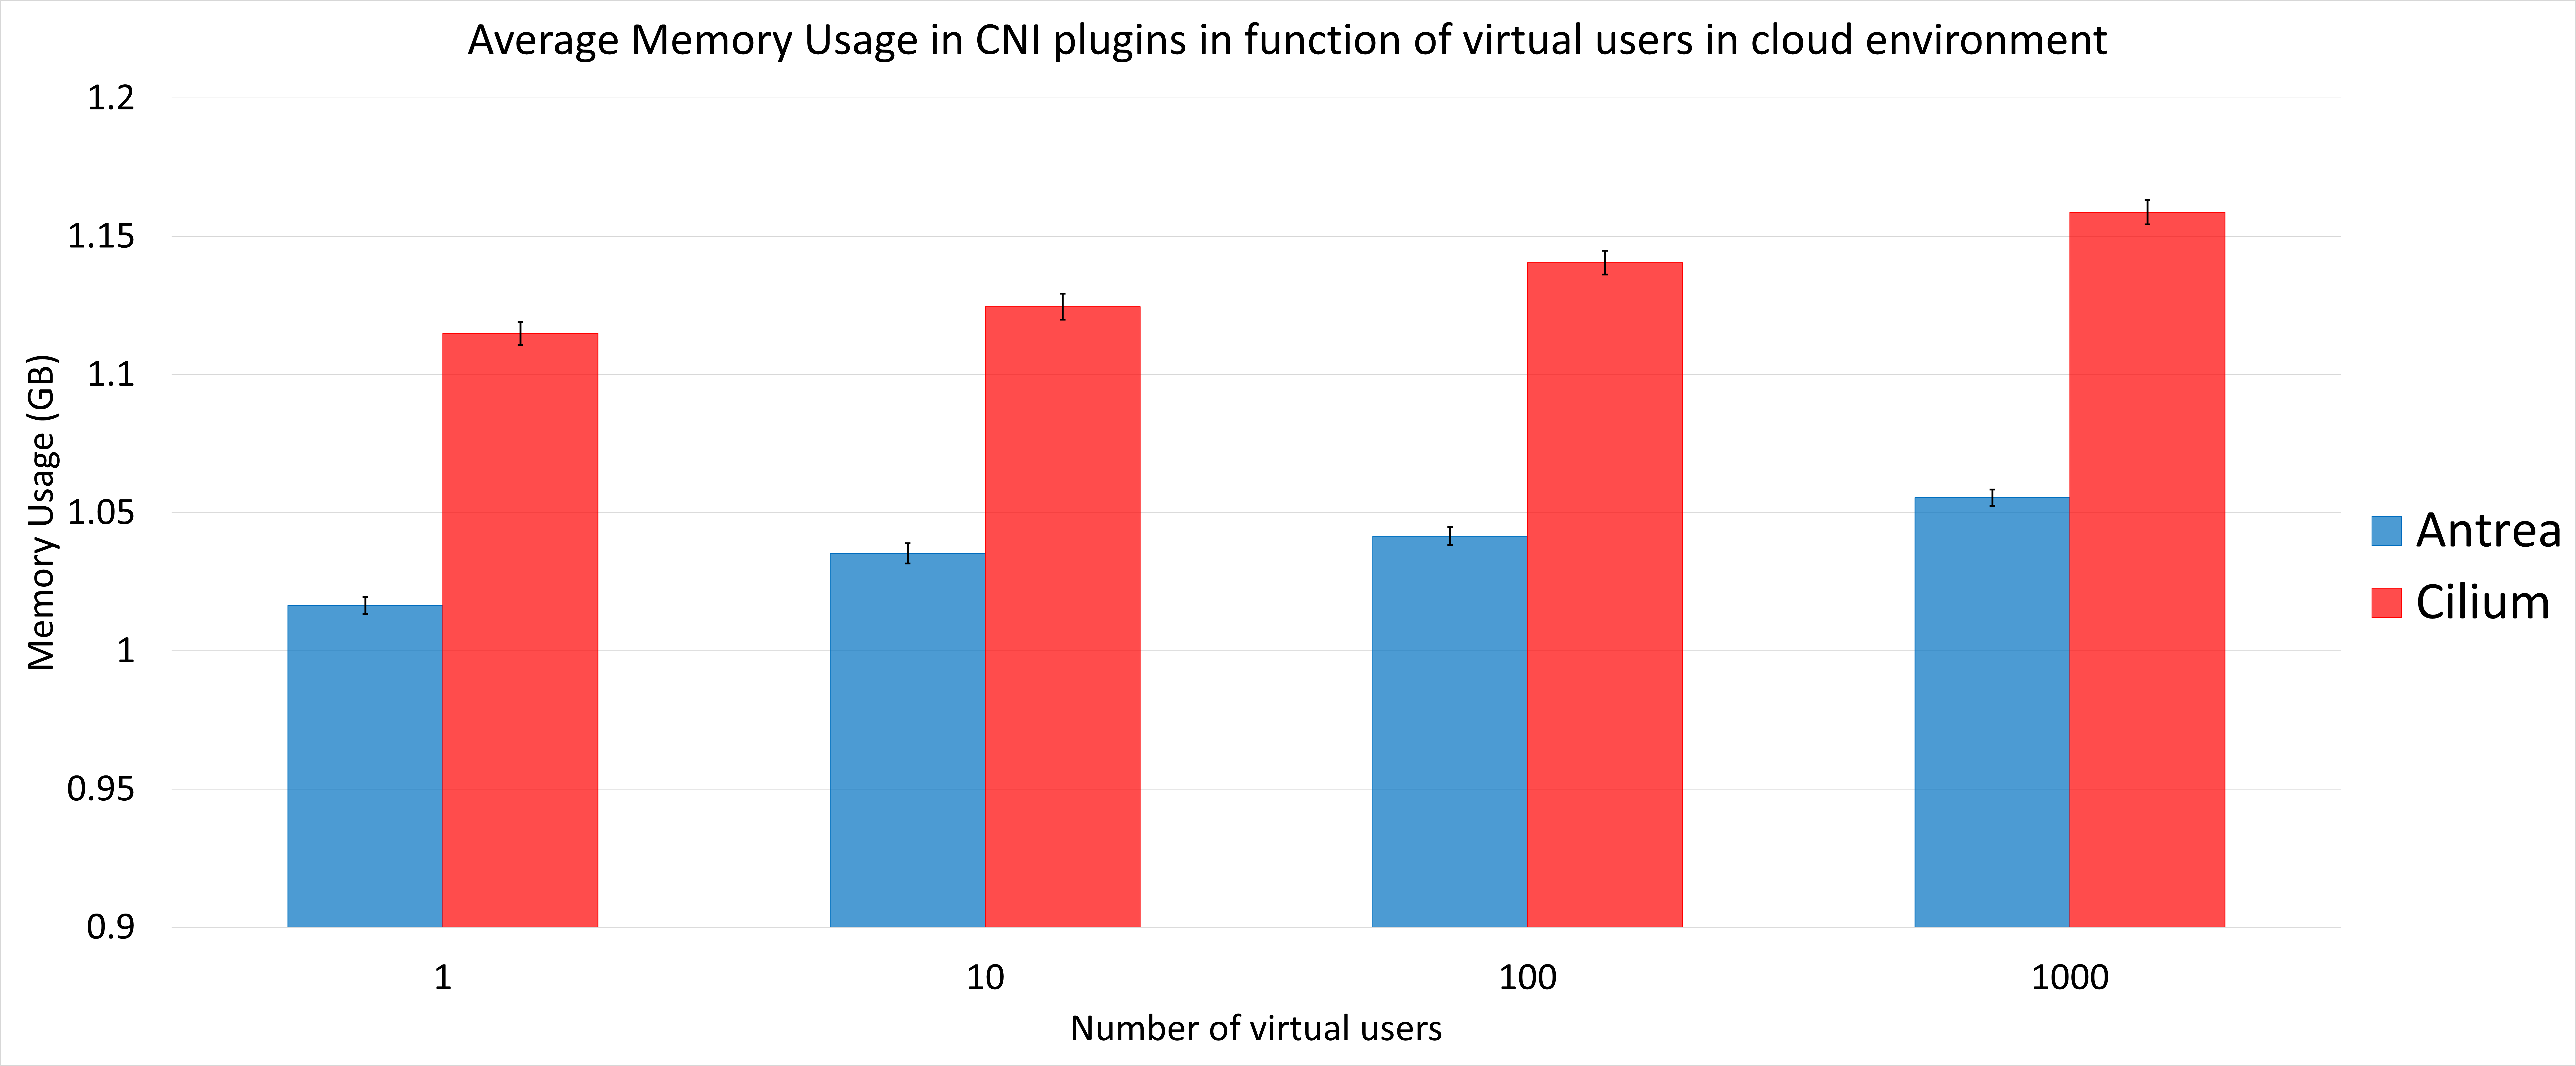
\includegraphics[width=\textwidth]{plots/traffic-splitting/memory_cloud.png}
        \caption{}
        \label{fig:memory_cloud_avg}
    \end{subfigure}
    
    \caption{Average resource utilization in ingress scenario with increasing virtual users in cloud environment, (a) CPU, (b) Memory}
    \label{fig:resource_cloud_avg}
\end{figure}

Comparing Figures~\ref{fig:resource_cloud_avg} and~\ref{fig:resource_local_avg}, it is evident that traffic management primarily impacts CPU usage rather than memory consumption, as memory usage shows egresser increases. In the cloud environment, Antrea demonstrates better resource efficiency, while in the local environment, Cilium consumes fewer resources. Antrea might use more CPU locally because there is an additional node, and the Gateway API NGINX pod is located on a different node (on the control plane) than the pod it forwards data to. This requires more resources to handle traffic across the cluster rather than within a single node.

\begin{figure}[H]
    \centering
    \begin{subfigure}[b]{1\textwidth}
        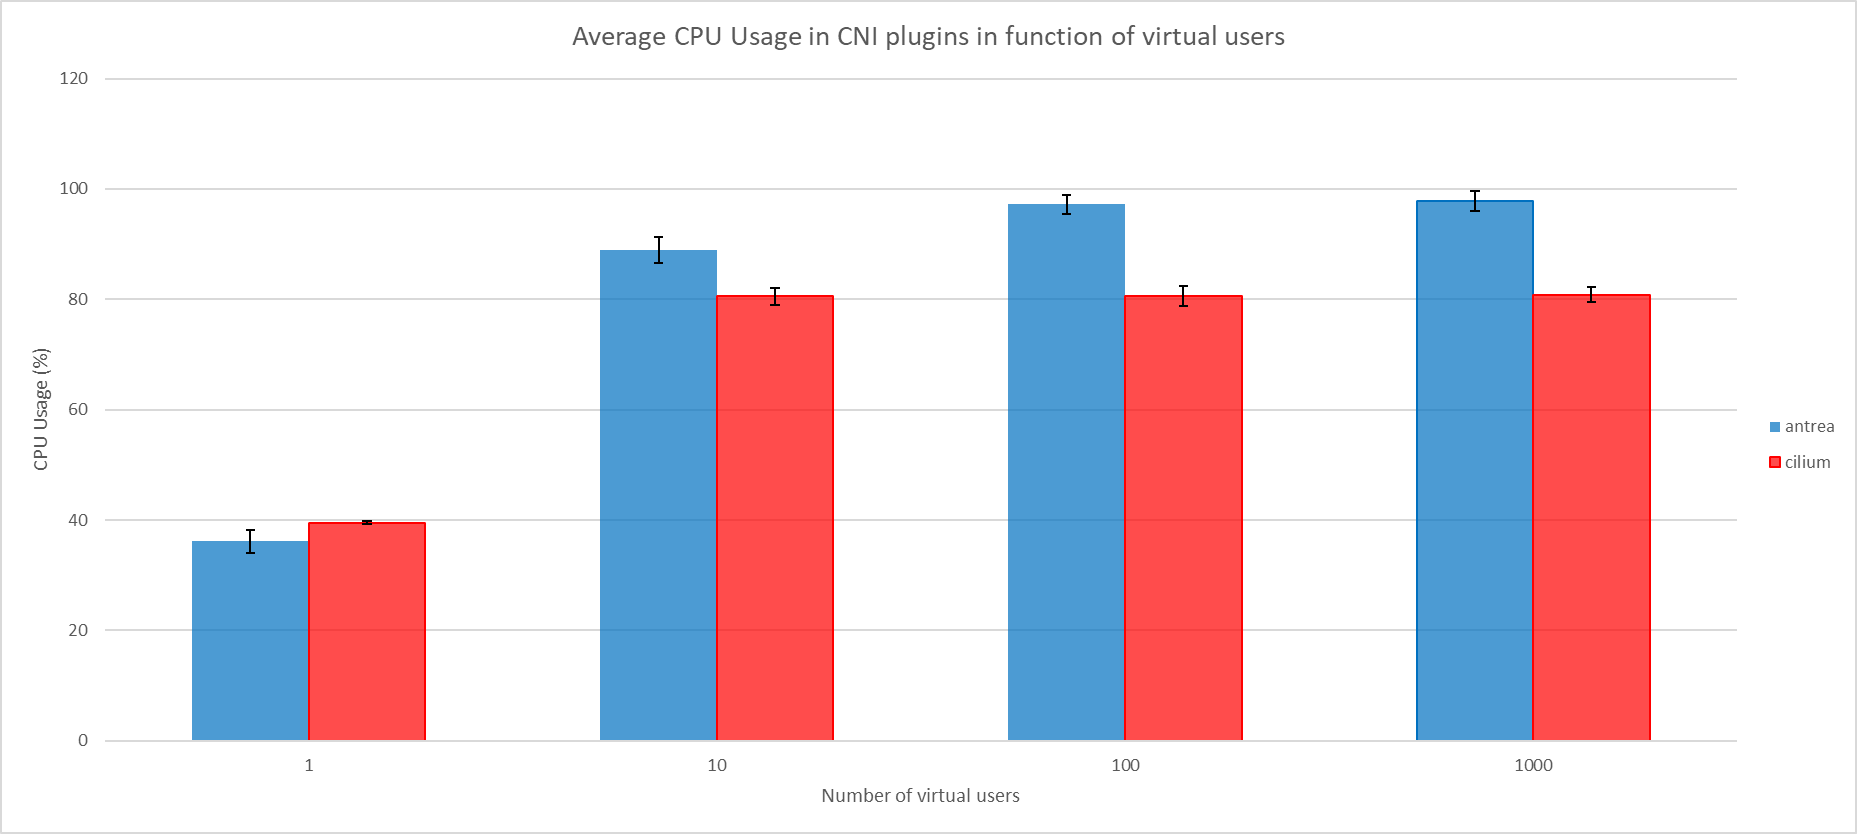
\includegraphics[width=\textwidth]{plots/traffic-splitting/cpu_local.png}
        \caption{}
        \label{fig:cpu_local_avg}
    \end{subfigure}
    \begin{subfigure}[b]{1\textwidth}
        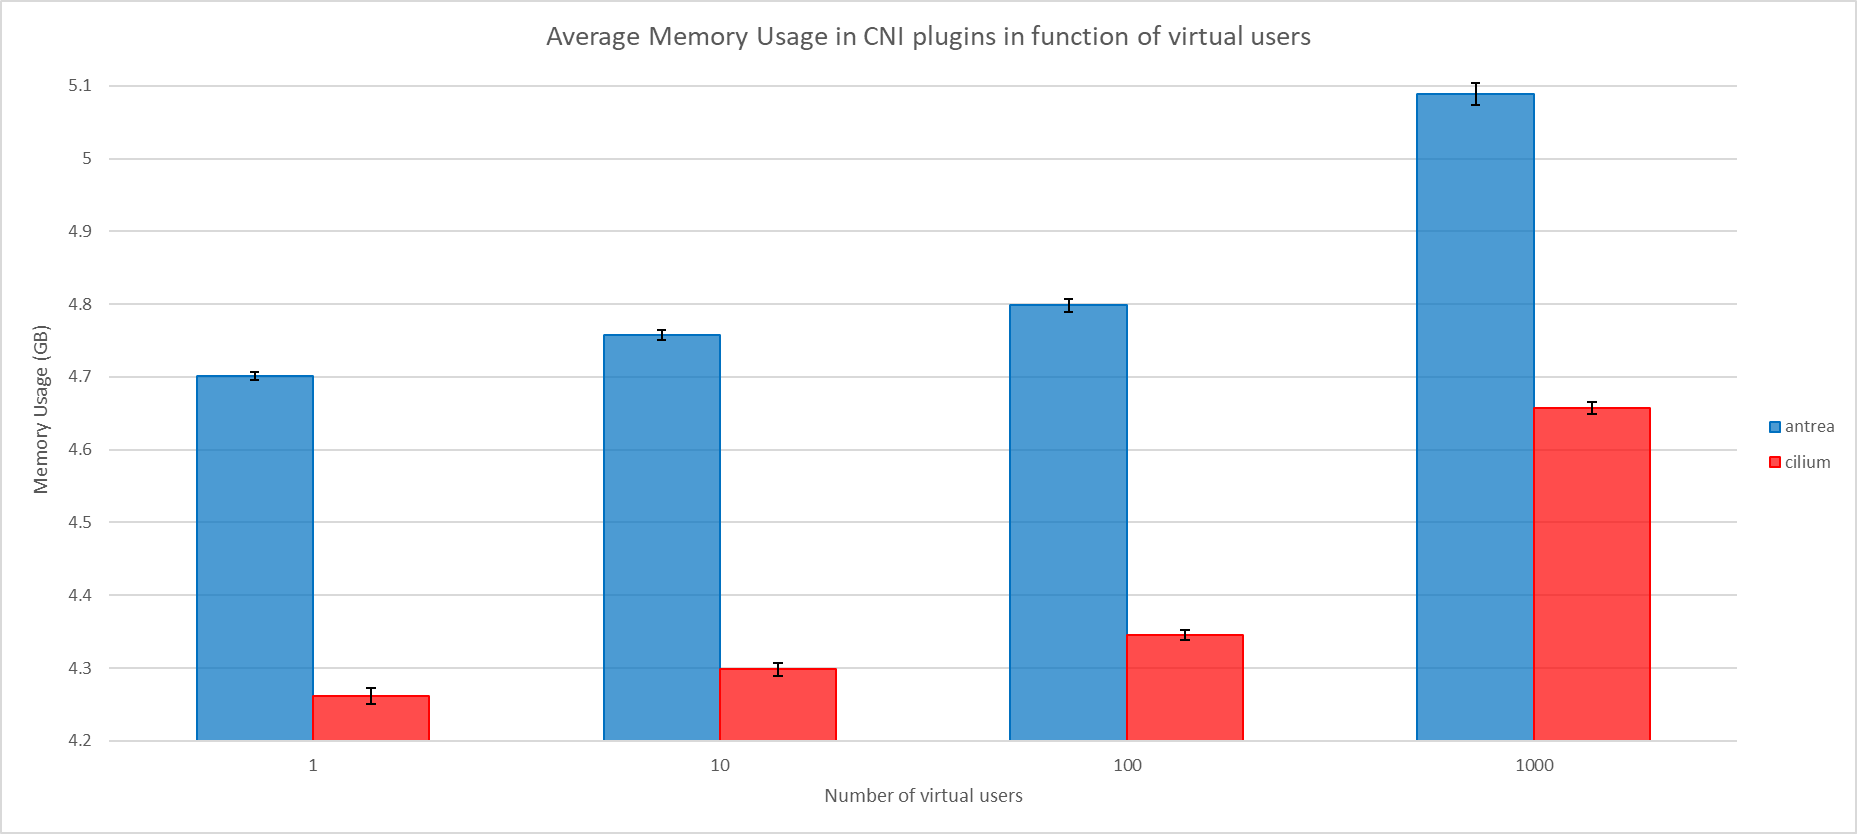
\includegraphics[width=\textwidth]{plots/traffic-splitting/memory_local.png}
        \caption{}
        \label{fig:memory_local_avg}
    \end{subfigure}
    
    \caption{Average resource utilization in ingress scenario with increasing virtual users in local environment, (a) CPU, (b) Memory}
    \label{fig:resource_local_avg}
\end{figure}

\subsubsection{Traffic splitting}
\label{sec:ingressTrafficSplitting}

When comparing traffic weighting accuracy in Figure~\ref{fig:vus_avg} with an increasing number of virtual users in a cloud environment, Antrea proves to be more precise, both when a single user makes a request and when a thousand users generate massive load. In a local environment, Cilium is more accurate in splitting traffic to the value specified in the HTTPRoute in every scenario except when only a single user is involved. Antrea, in the local environment, shows wider confidence intervals, and the distance from the reference point is higher compared to Cilium, making it less effective during high-load periods.


\begin{figure}[H]
    \centering
    \begin{subfigure}[b]{1\textwidth}
        
\includegraphics[width=\textwidth]{plots/traffic-splitting/vus_cloud_all.png}
        \caption{}
        \label{fig:vus_cloud_avg}
    \end{subfigure}
    \begin{subfigure}[b]{1\textwidth}
        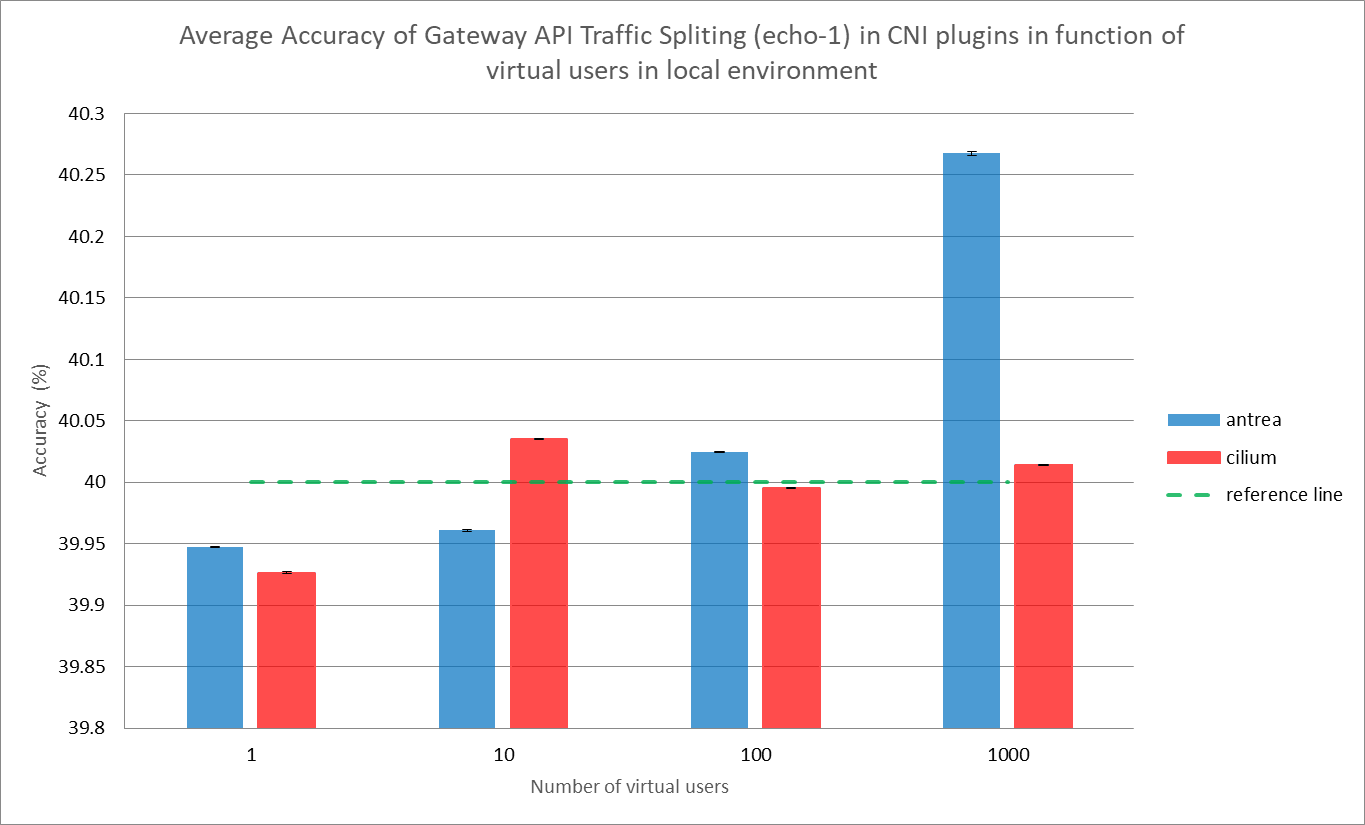
\includegraphics[width=\textwidth]{plots/traffic-splitting/vus_local_all.png}
        \caption{}
        \label{fig:vus_local_avg}
    \end{subfigure}
    
    \caption{Average traffic splitting accuracy in ingress scenario with increasing virtual users (a) cloud, (b) local}
    \label{fig:vus_avg}
\end{figure}


Analyzing the plots in Figure~\ref{fig:avg_vus}, we observe overlapping confidence intervals in all cases, indicating some variability in the results. However, when averaging the values, it becomes clear that Cilium performs better, particularly when the number of virtual users (VUs) is either one or a thousand. The distance to reference points is illustrated in Figure~\ref{fig:referencesIngress}. Although the overlapping confidence intervals suggest statistical uncertainty, the average values show that Cilium achieves higher accuracy in traffic weighting compared to Antrea and the NGINX test case.


\begin{figure}[H]
    \centering
    \begin{subfigure}[b]{0.85\textwidth}
        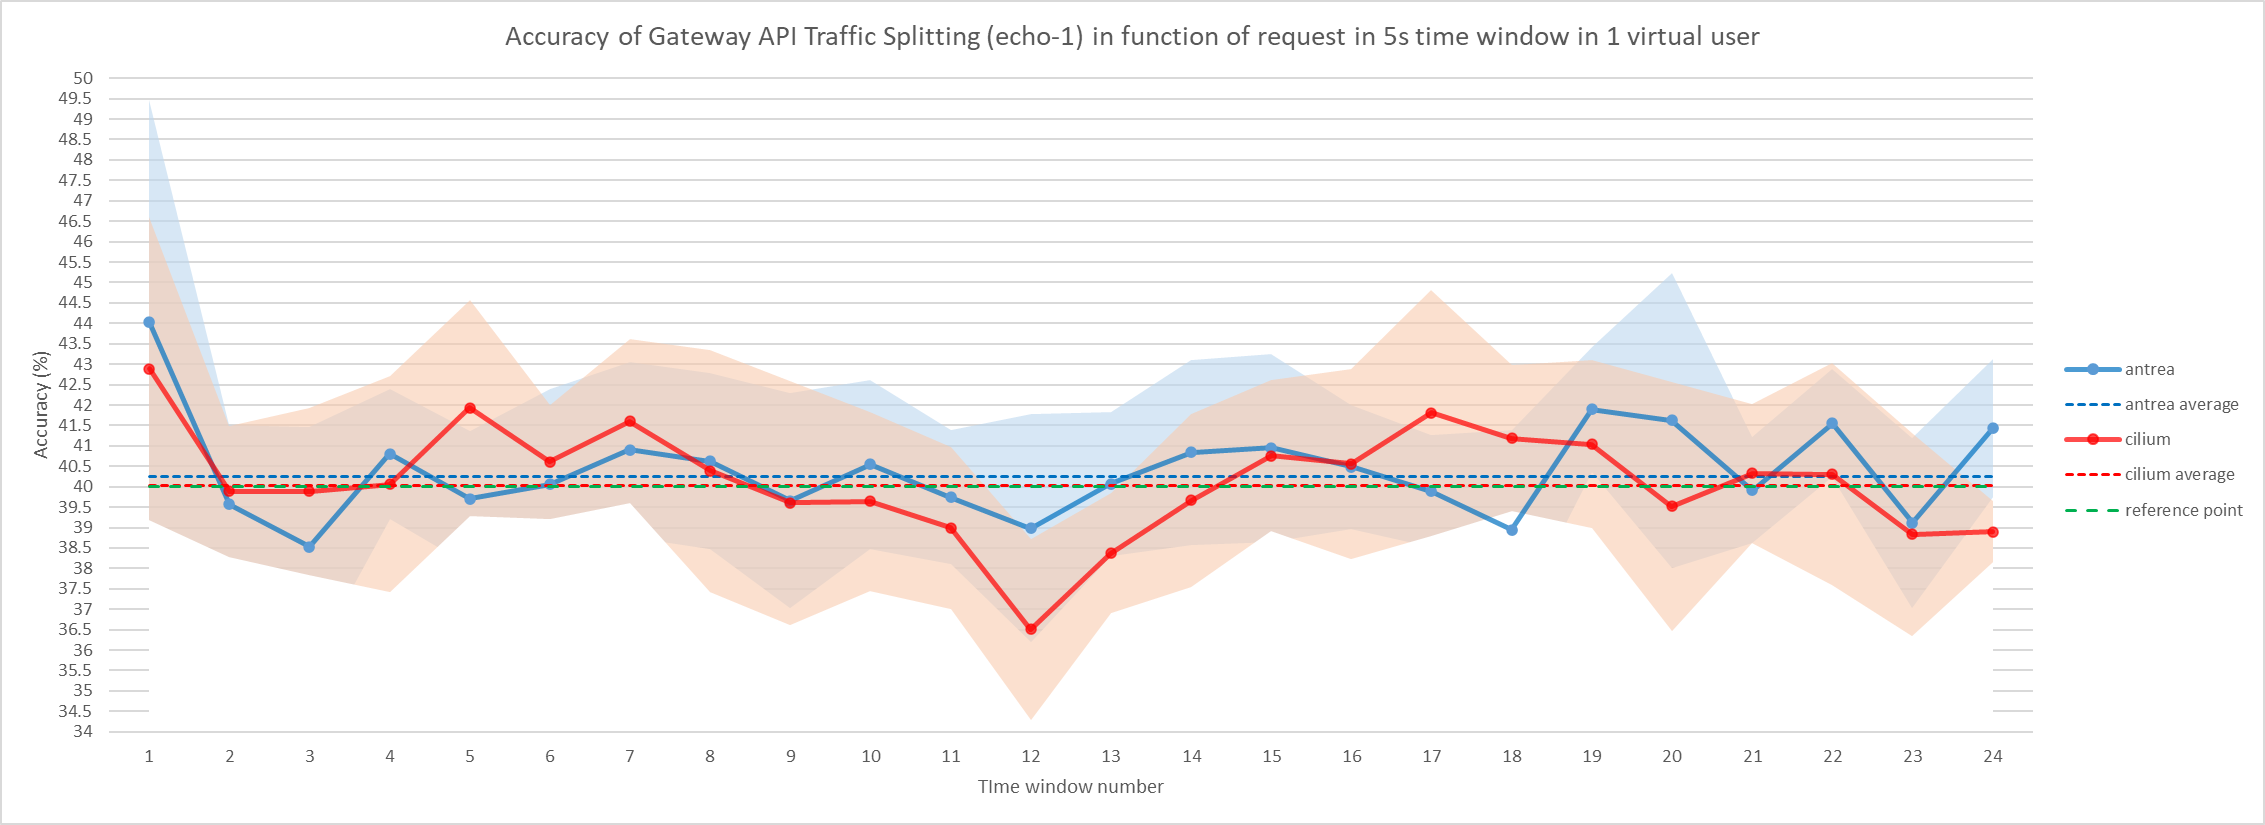
\includegraphics[width=\textwidth]{plots/traffic-splitting/time_window_5_1vu_cloud.png}
        \label{fig:time_window_1vu}
    \end{subfigure}

    \vspace{-0.5cm}

    \begin{subfigure}[b]{0.85\textwidth}
        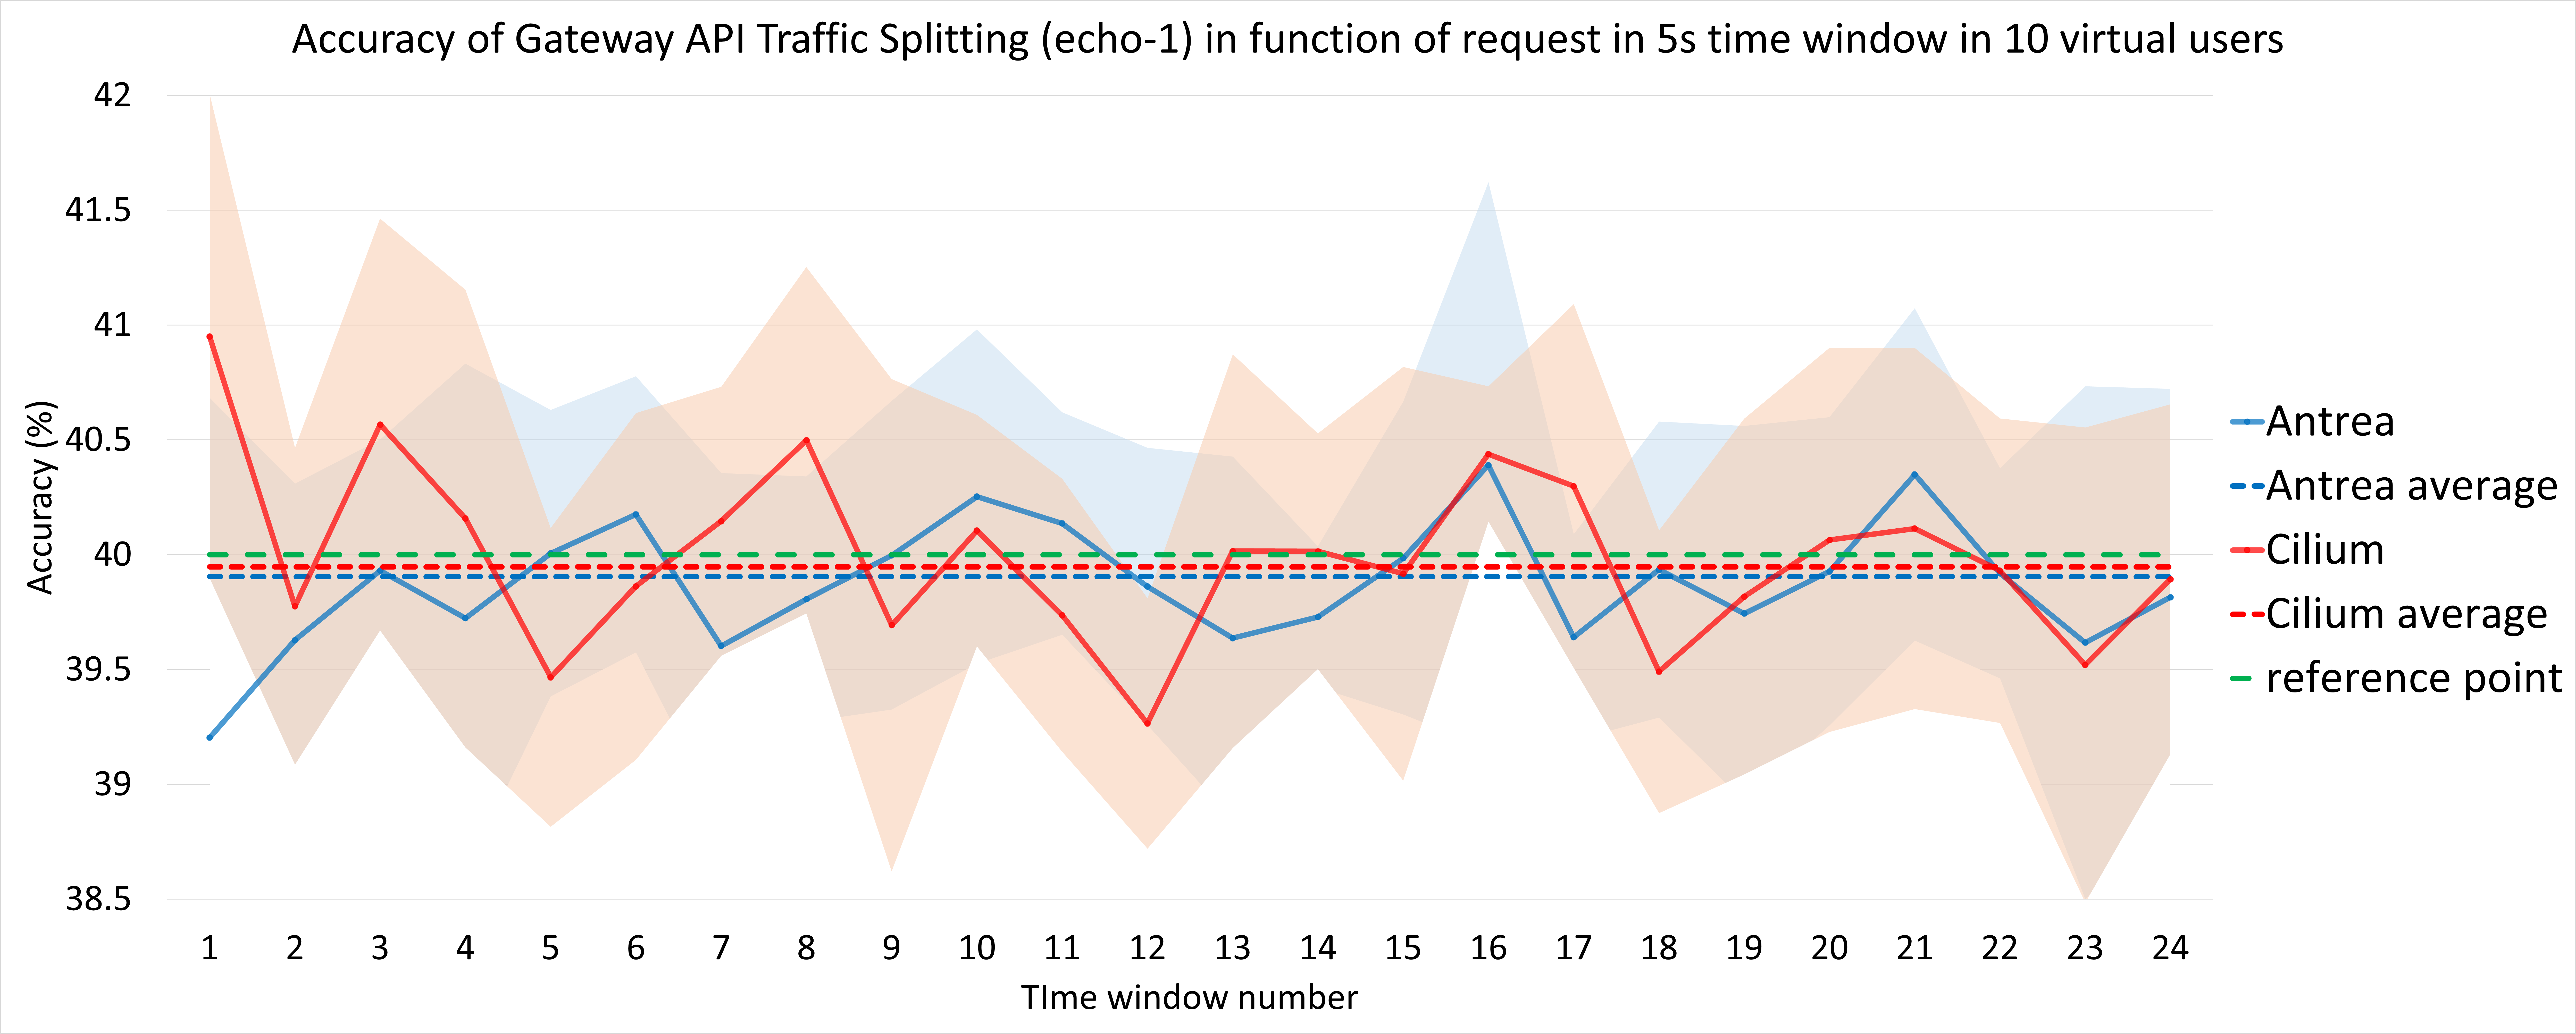
\includegraphics[width=\textwidth]{plots/traffic-splitting/time_window_5_10vu_cloud.png}
        \label{fig:time_window_10vu}
    \end{subfigure}

    \vspace{-0.5cm}

    \begin{subfigure}[b]{0.85\textwidth}
        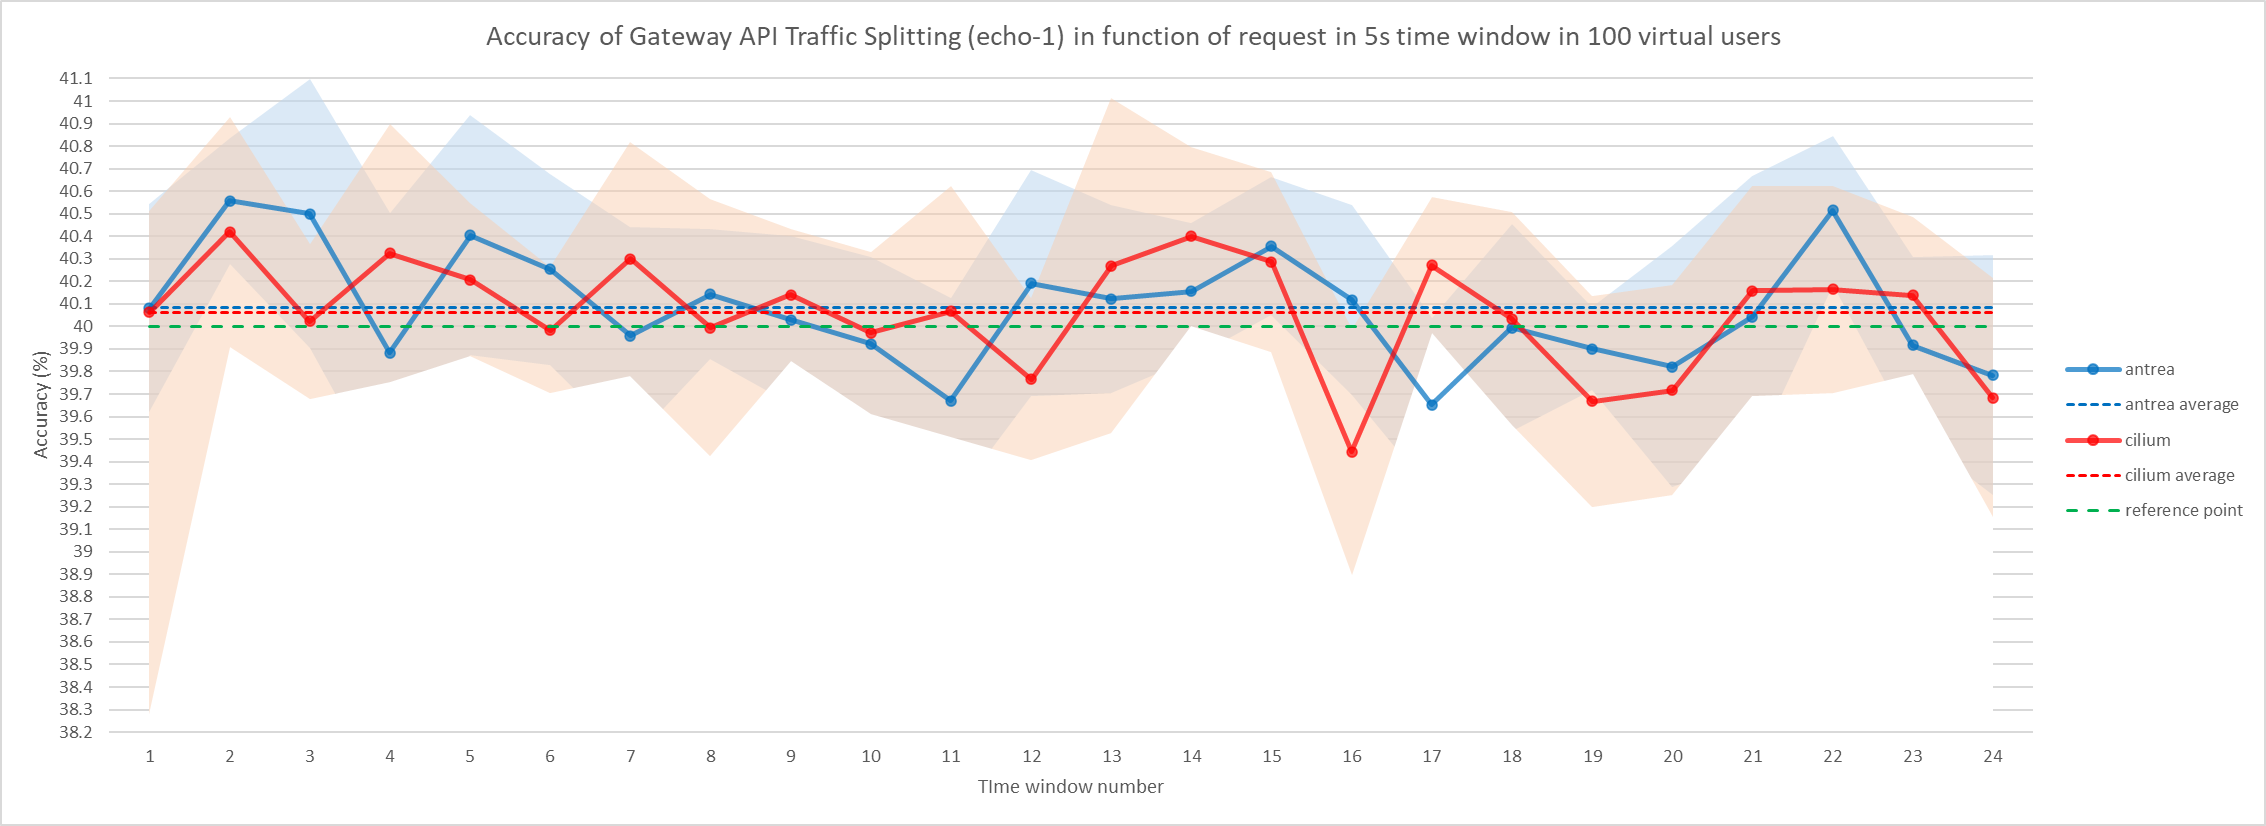
\includegraphics[width=\textwidth]{plots/traffic-splitting/time_window_5_100vu_cloud.png}
        \label{fig:time_window_100vu}
    \end{subfigure}

    \vspace{-0.5cm}

    \begin{subfigure}[b]{0.85\textwidth}
        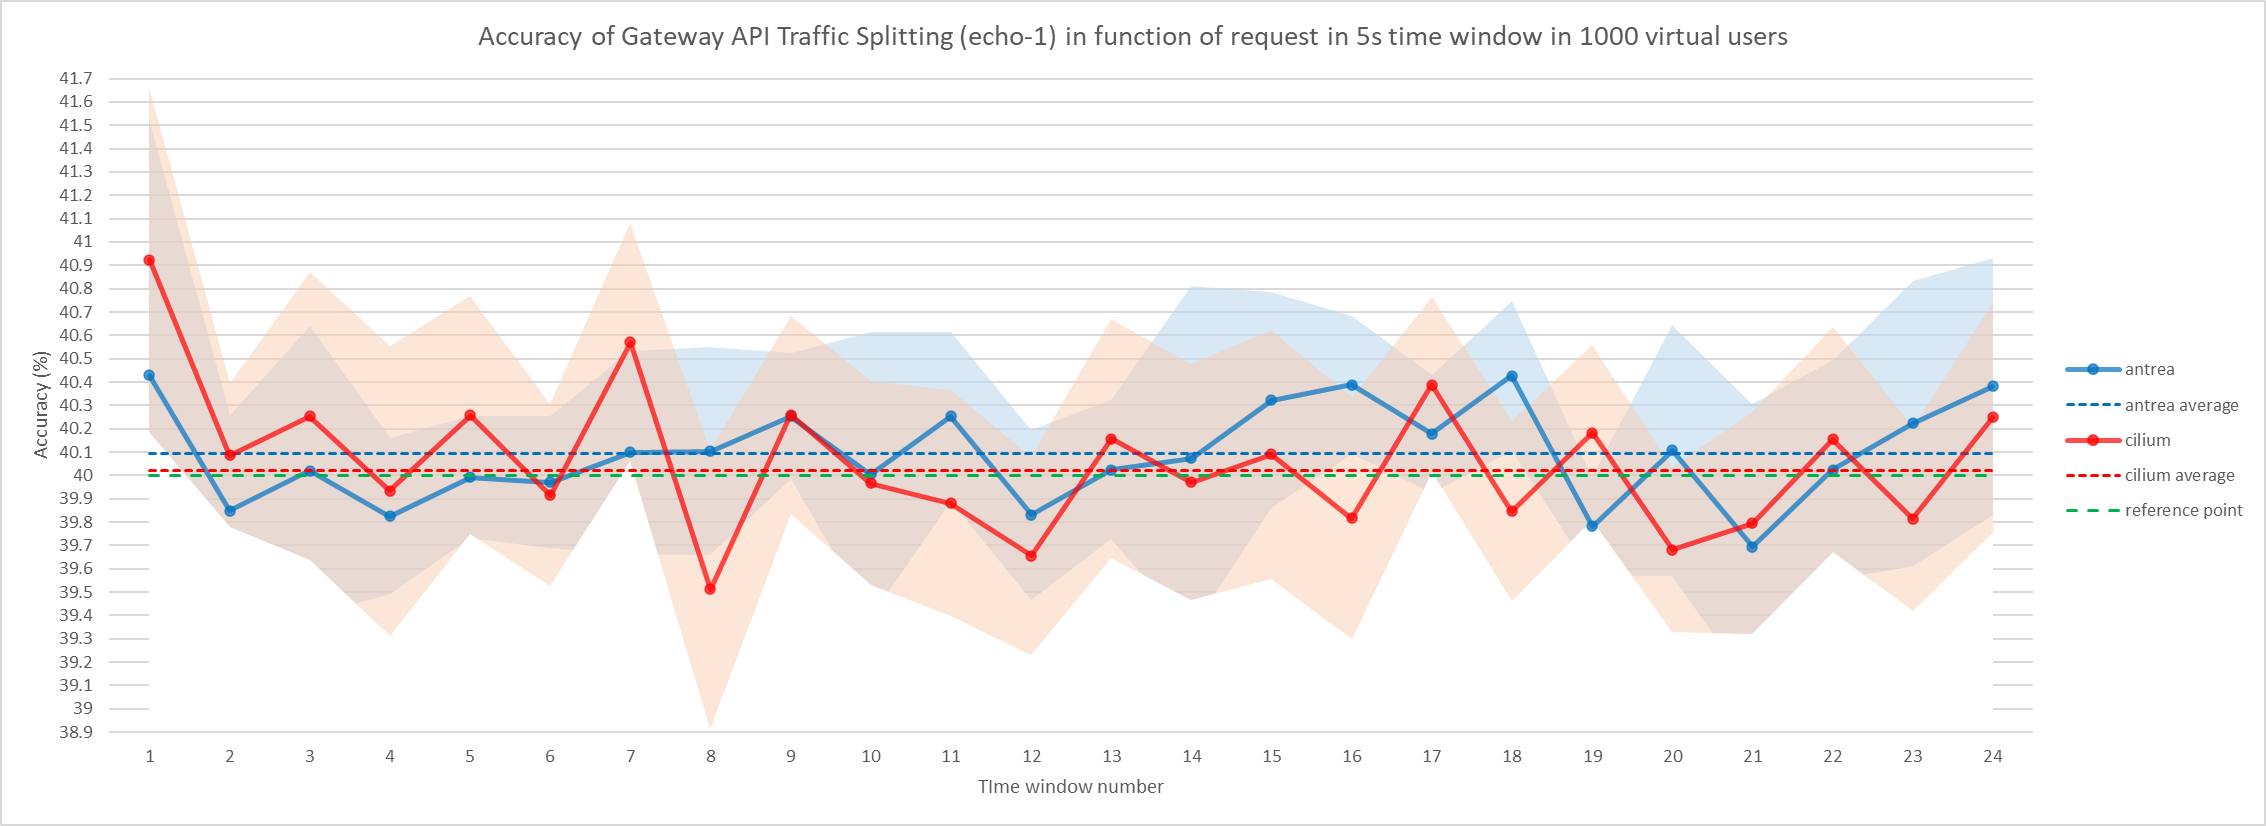
\includegraphics[width=\textwidth]{plots/traffic-splitting/time_window_5_1000vu_cloud.png}
        \label{fig:time_window_1000vu}
    \end{subfigure}

    \vspace{-0.3cm}

    \caption{Average traffic splitting ratio in function of five second request time windows with increasing virtual users; one, ten, a hundred and a thousand users}
    \label{fig:avg_vus}
\end{figure}



\begin{figure}[H]
    \centering
    \begin{subfigure}[b]{0.49\textwidth}
        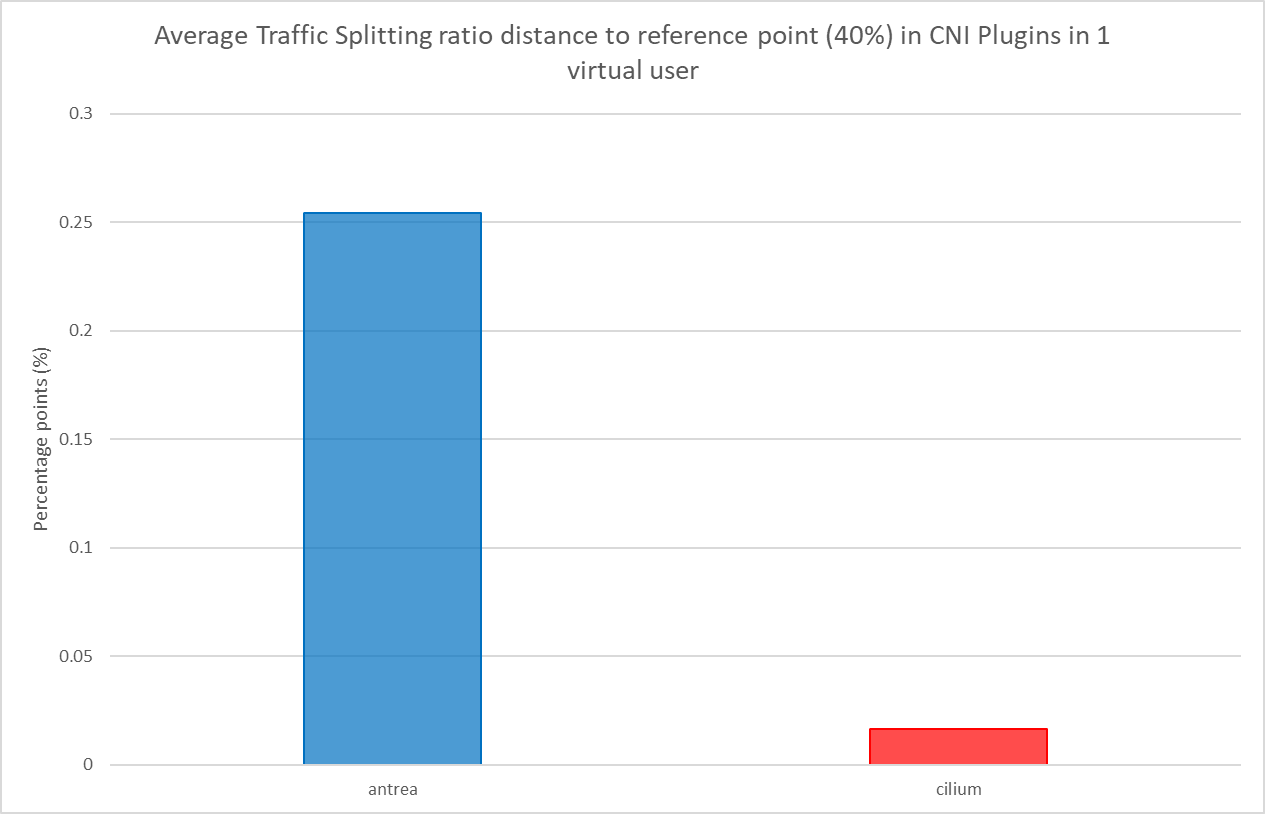
\includegraphics[width=\textwidth]{plots/traffic-splitting/time_window_5_1vu_reference_cloud.png}
        \label{fig:reference_1vu}
        \caption{}
    \end{subfigure}
    \begin{subfigure}[b]{0.49\textwidth}
        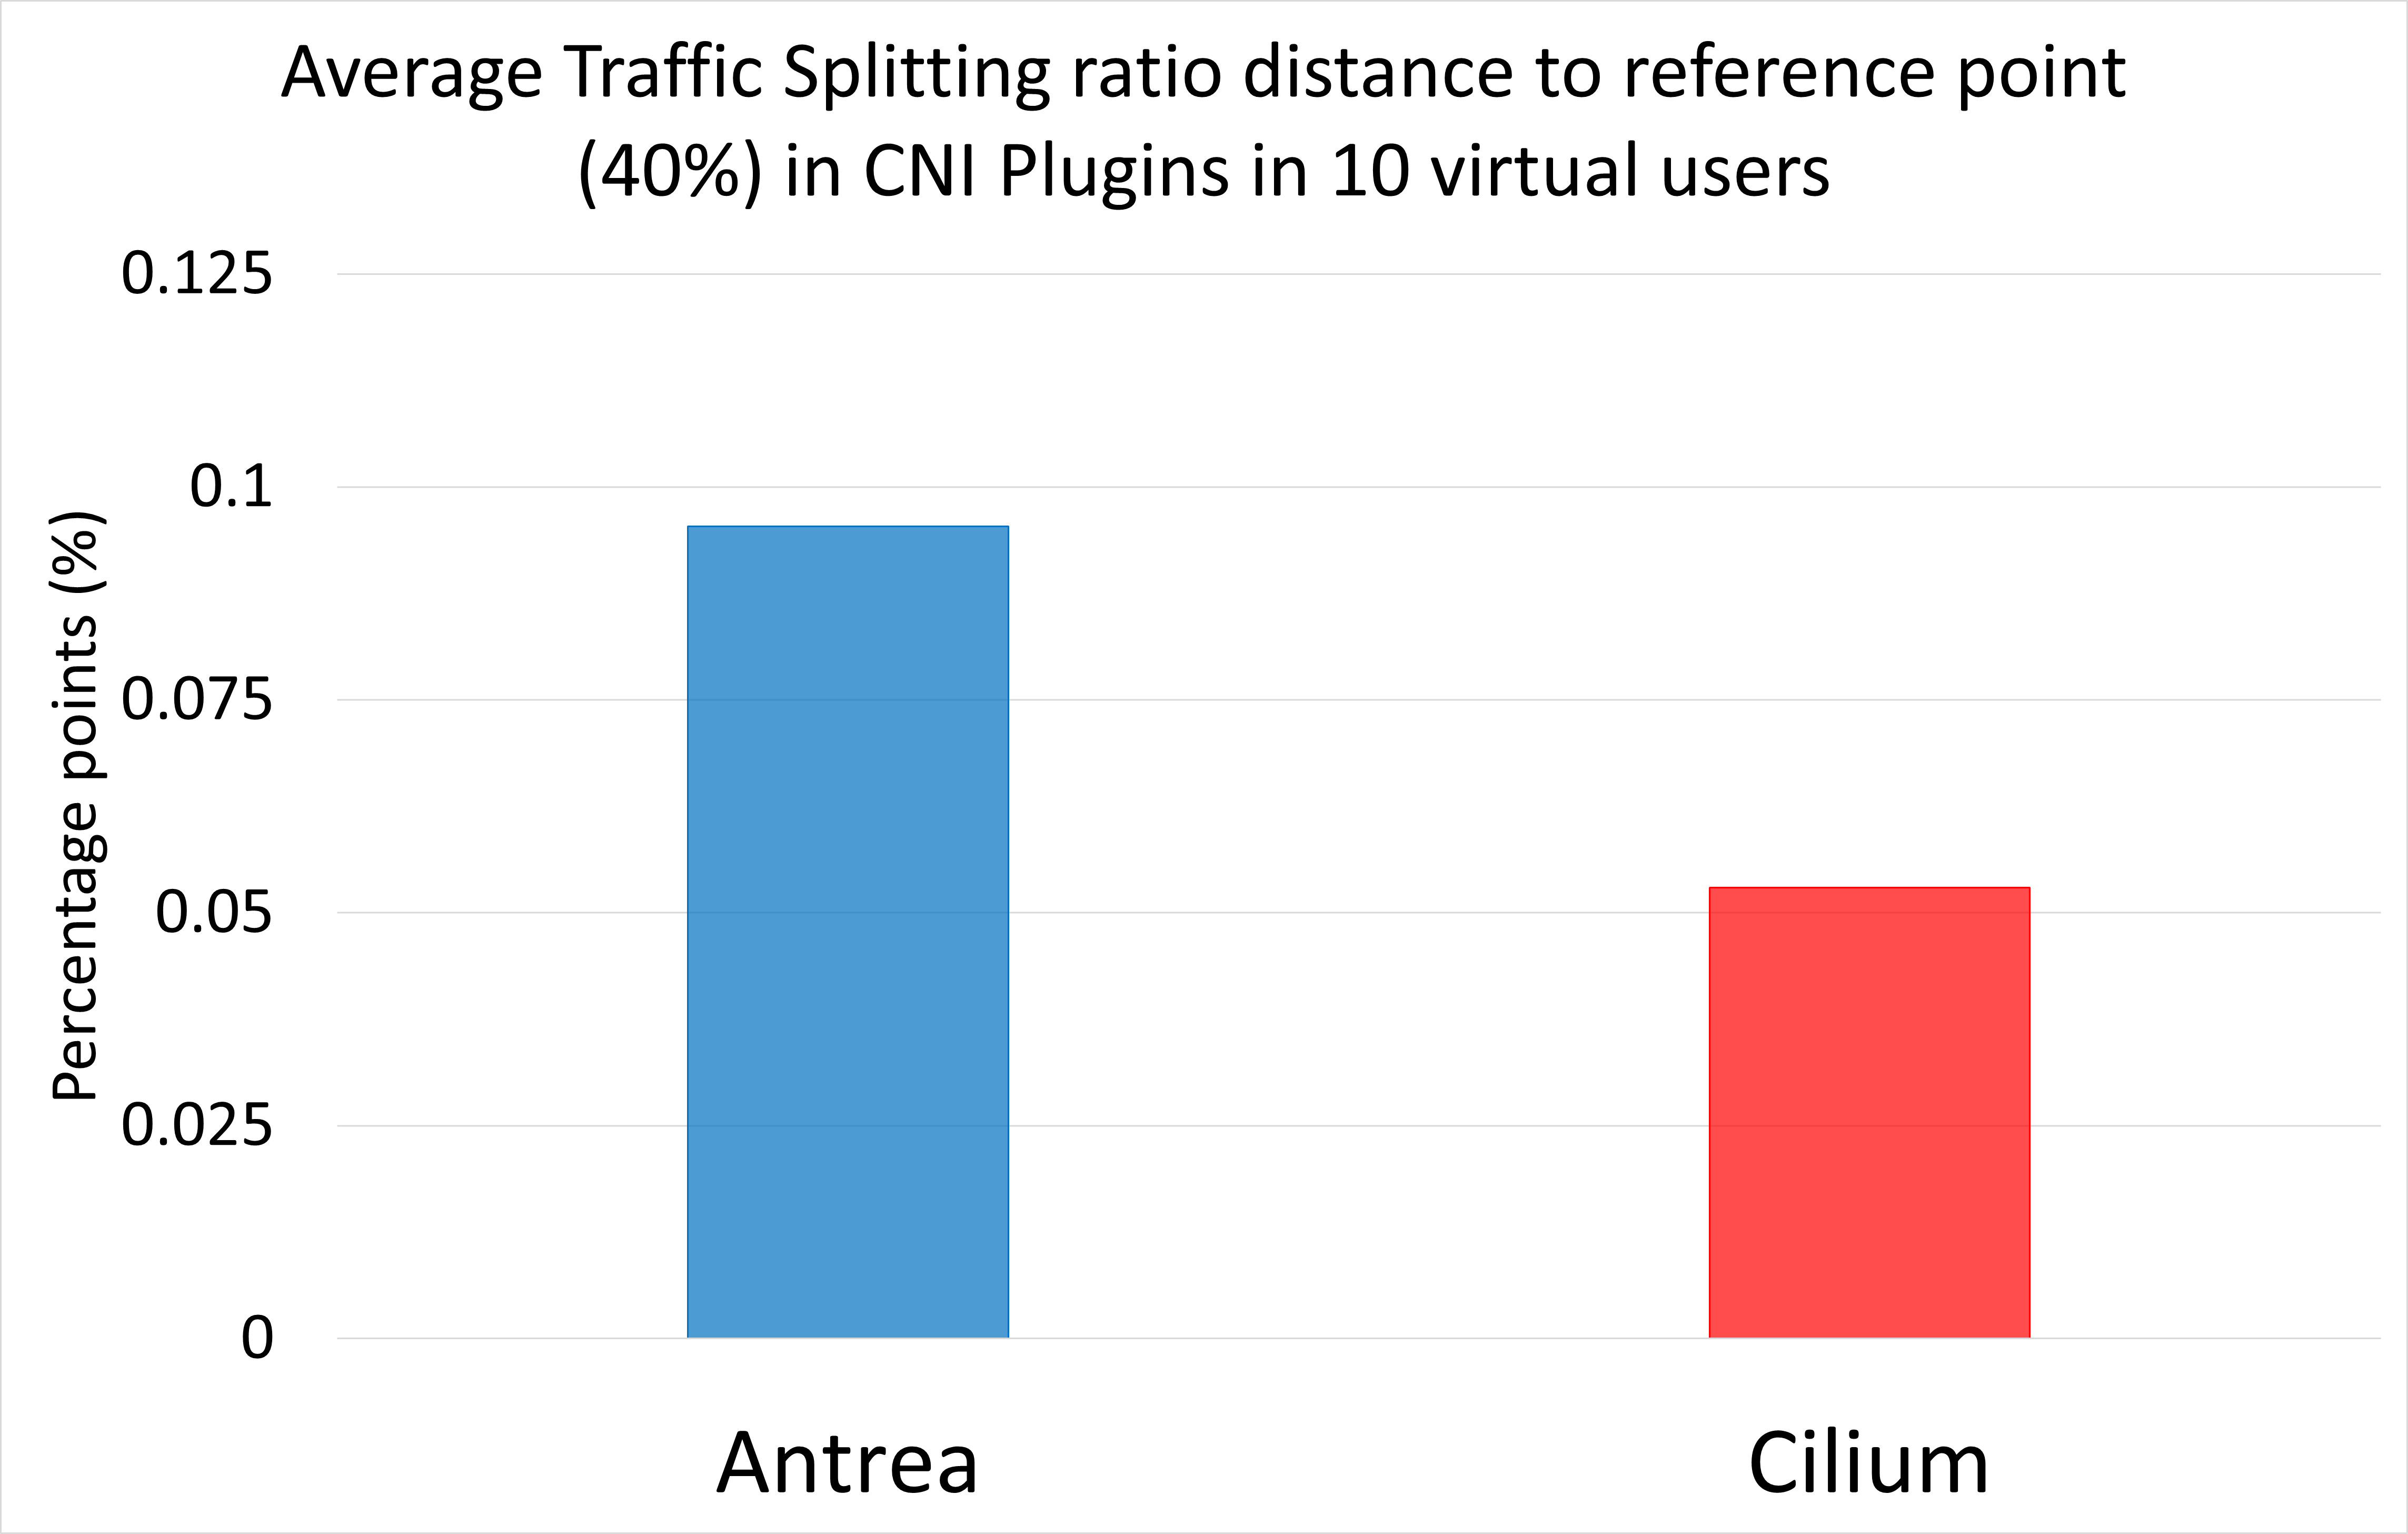
\includegraphics[width=\textwidth]{plots/traffic-splitting/time_window_5_10vu_reference_cloud.png}
        \label{fig:reference_10vu}
        \caption{}
    \end{subfigure}

    \vspace{0.5cm}

    \begin{subfigure}[b]{0.49\textwidth}
        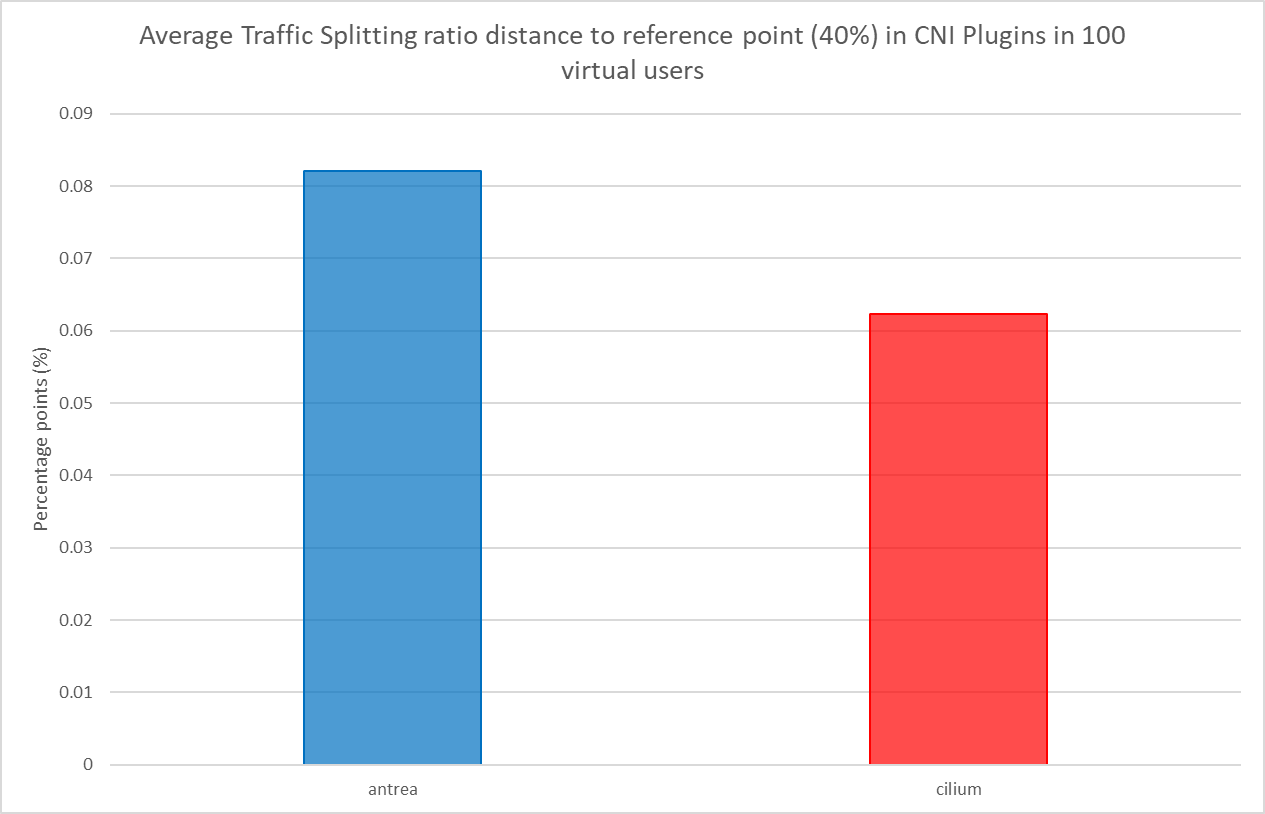
\includegraphics[width=\textwidth]{plots/traffic-splitting/time_window_5_100vu_reference_cloud.png}
        \label{fig:reference_100vu}
        \caption{}
    \end{subfigure}
    \begin{subfigure}[b]{0.49\textwidth}
        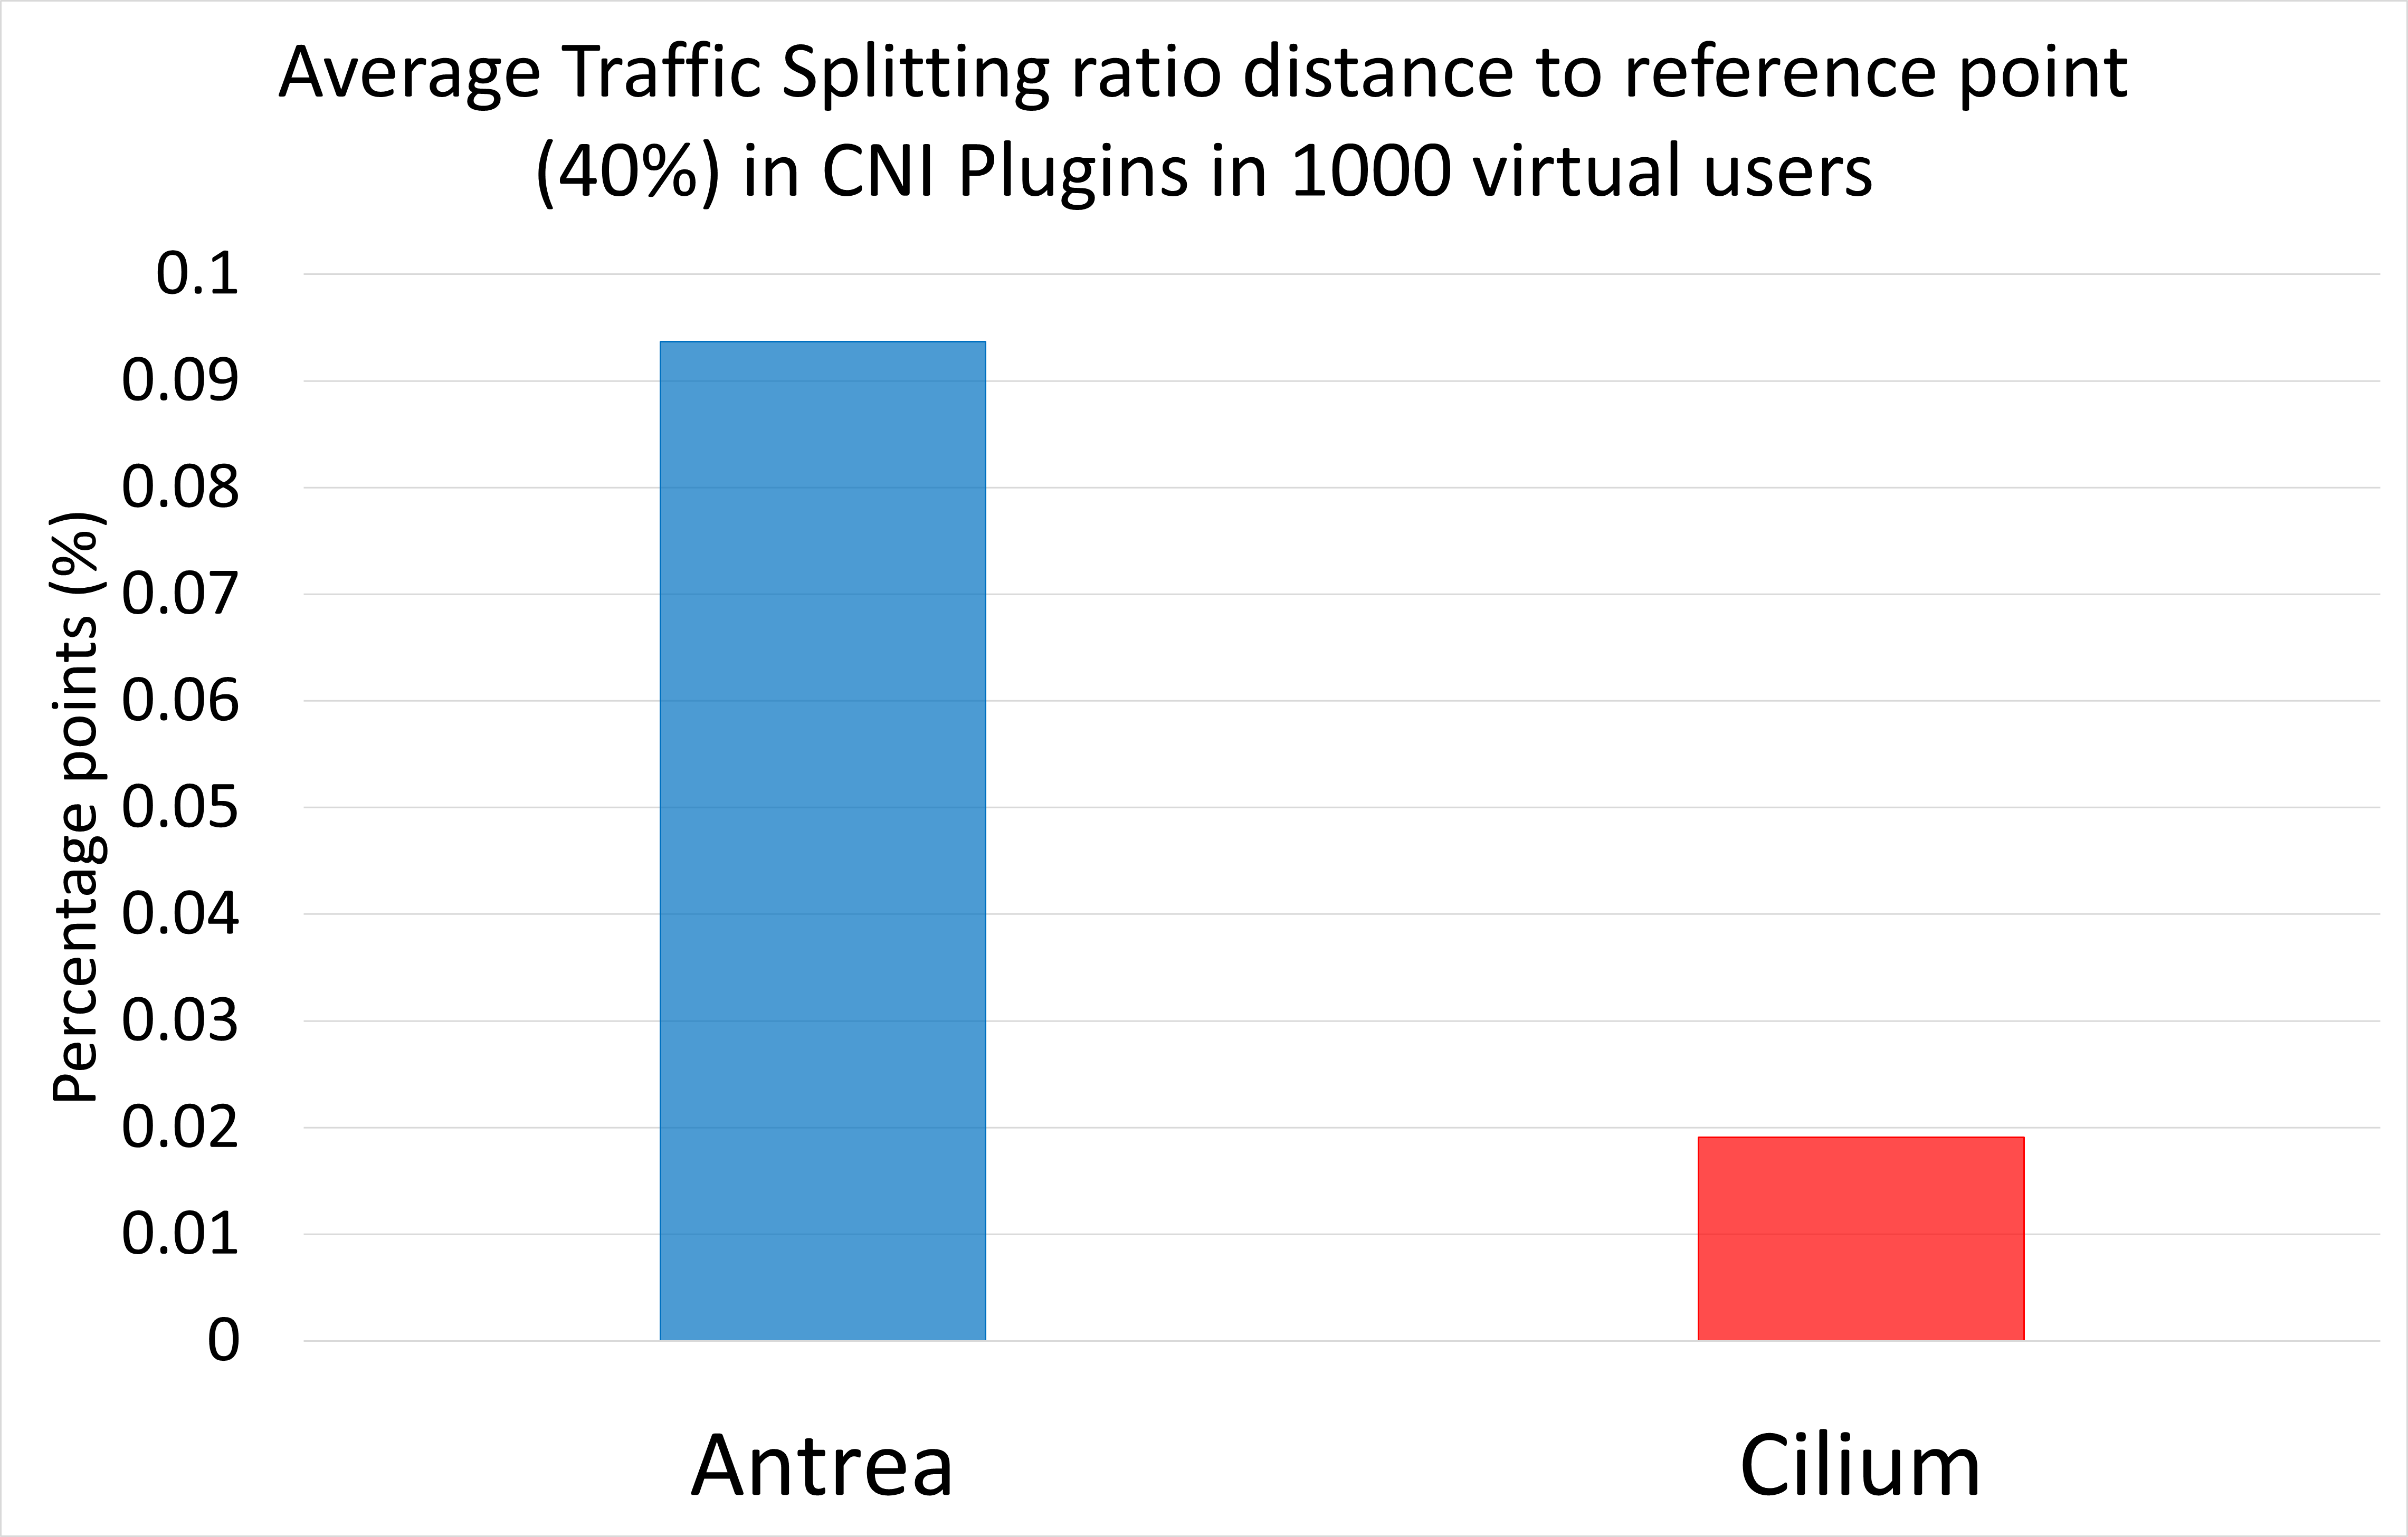
\includegraphics[width=\textwidth]{plots/traffic-splitting/time_window_5_1000vu_reference_cloud.png}
        \label{fig:reference_1000vu}
        \caption{}
    \end{subfigure}

    \caption{Average traffic splitting ratio distance to reference point in increasing virtual users, (a) one, (b) ten, (c) hundred, (d) thousand }
    \label{fig:referencesIngress}
\end{figure}

\chapter{Egress Scenario Comparison}
\label{cha:compare_egress}

%---------------------------------------------------------------------------

\section{Resource Utilization}
\label{sec:resources}


%---------------------------------------------------------------------------

\section{Throughput}
\label{sec:throughput}



%---------------------------------------------------------------------------

\section{Round Trip Time}
\label{sec:rtt}

%---------------------------------------------------------------------------




% \chapter{Ingress Scenario Comparison}
\label{cha:ingress_compare}

W rozdziale tym przedstawiono podstawowe informacje dotyczące struktury prostych plików \LaTeX a. Omówiono również metody kompilacji plików z zastosowaniem programów \emph{latex} oraz \emph{pdflatex}.

%---------------------------------------------------------------------------

\section{Resource Utilization}
\label{sec:traffic_concept}

Plik \LaTeX owy jest plikiem tekstowym, który oprócz tekstu zawiera polecenia formatujące ten tekst (analogicznie do języka HTML). Plik składa się z dwóch części:
\begin{enumerate}%[1)]
\item Preambuły -- określającej klasę dokumentu oraz zawierającej m.in. polecenia dołączającej dodatkowe pakiety;

\item Części głównej -- zawierającej zasadniczą treść dokumentu.
\end{enumerate}


\begin{lstlisting}

\end{document}
\end{lstlisting}

Nie ma żadnych przeciwskazań do tworzenia dokumentów w~\LaTeX u w~języku polskim. Plik źródłowy jest zwykłym plikiem tekstowym i~do jego przygotowania można użyć dowolnego edytora tekstów, a~polskie znaki wprowadzać używając prawego klawisza \texttt{Alt}. Jeżeli po kompilacji dokumentu polskie znaki nie są wyświetlane poprawnie, to na 95\% źle określono sposób kodowania znaków (należy zmienić opcje wykorzystywanych pakietów).


%---------------------------------------------------------------------------

\section{Traffic Splitting}
\label{sec:traffic_mngmnt}


Załóżmy, że przygotowany przez nas dokument zapisany jest w pliku \texttt{test.tex}. Kolejno wykonane poniższe polecenia (pod warunkiem, że w pierwszym przypadku nie wykryto błędów i kompilacja zakończyła się sukcesem) pozwalają uzyskać nasz dokument w formacie pdf:
\begin{lstlisting}
latex test.tex
dvips test.dvi -o test.ps
ps2pdf test.ps
\end{lstlisting}
%
lub za pomocą PDF\LaTeX:
\begin{lstlisting}
pdflatex test.tex
\end{lstlisting}

Przy pierwszej kompilacji po zmiane tekstu, dodaniu nowych etykiet itp., \LaTeX~tworzy sobie spis rozdziałów, obrazków, tabel itp., a dopiero przy następnej kompilacji korzysta z tych informacji.

W pierwszym przypadku rysunki powinny być przygotowane w~formacie eps, a~w~drugim w~formacie pdf. Ponadto, jeżeli używamy polecenia \texttt{pdflatex test.tex} można wstawiać grafikę bitową (np. w formacie jpg).


\subsection{Virtual Users}
\label{sec:vus}

\subsection{Time Window}
\label{sec:time_wind}


% \chapter{Conclusion}
\label{cha:conclusion}
% \chapter{eBPF in Traffic Engineering}
% \label{cha:ebpf}

% %---------------------------------------------------------------------------

% \section{The Concept of Traffic Engineering}
% \label{sec:traffic_concept}

% %---------------------------------------------------------------------------

% \section{Network Traffic Management in Kubernetes}
% \label{sec:traffic_mngmnt}


% %---------------------------------------------------------------------------

% \section{Ingress and Egress Traffic Management in Kubernetes}
% \label{sec:ing_egr_traffic_mgmnt}
% %---------------------------------------------------------------------------

% \include{chapters/chapter9}

\bibliographystyle{unsrt}
\bibliography{bibliography}
All figures in this document were created using Lucidchart for diagrams and Microsoft Excel for data visualization \cite{LucidApp}\cite{Excel}.
Icon sources \cite{CloudIcon}\cite{CloudIcon2}\cite{EtcdIcon}\cite{K8sIcons}\cite{KindIcon}\cite{PersonIcon}\cite{TerraformIcon}\cite{AnsibleIcon}\cite{DockerIcon}\cite{AzureIcons}.




\end{document}
